%%
%% This is file `sample-sigconf.tex',
%% generated with the docstrip utility.
%%
%% The original source files were:
%%
%% samples.dtx  (with options: `all,proceedings,bibtex,sigconf')
%% 
%% IMPORTANT NOTICE:
%% 
%% For the copyright see the source file.
%% 
%% Any modified versions of this file must be renamed
%% with new filenames distinct from sample-sigconf.tex.
%% 
%% For distribution of the original source see the terms
%% for copying and modification in the file samples.dtx.
%% 
%% This generated file may be distributed as long as the
%% original source files, as listed above, are part of the
%% same distribution. (The sources need not necessarily be
%% in the same archive or directory.)
%%
%%
%% Commands for TeXCount
%TC:macro \cite [option:text,text]
%TC:macro \citep [option:text,text]
%TC:macro \citet [option:text,text]
%TC:envir table 0 1
%TC:envir table* 0 1
%TC:envir tabular [ignore] word
%TC:envir displaymath 0 word
%TC:envir math 0 word
%TC:envir comment 0 0
%%
%% The first command in your LaTeX source must be the \documentclass
%% command.
%%
%% For submission and review of your manuscript please change the
%% command to \documentclass[manuscript, screen, review]{acmart}.
%%
%% When submitting camera ready or to TAPS, please change the command
%% to \documentclass[sigconf]{acmart} or whichever template is required
%% for your publication.
%%
%%
\documentclass[sigconf]{acmart}
%%
%% \BibTeX command to typeset BibTeX logo in the docs
% \AtBeginDocument{%
%   \providecommand\BibTeX{{%
%     Bib\TeX}}}

%% Rights management information.  This information is sent to you
%% when you complete the rights form.  These commands have SAMPLE
%% values in them; it is your responsibility as an author to replace
%% the commands and values with those provided to you when you
%% complete the rights form.
% \setcopyright{acmlicensed}
% \copyrightyear{2025}
% \acmYear{2025}
% \acmDOI{XXXXXXX.XXXXXXX}
%% These commands are for a PROCEEDINGS abstract or paper.
% \acmConference[Conference acronym 'XX]{Make sure to enter the correct
%   conference title from your rights confirmation email}{June 03--05,
%   2025}{Houston, TX}
%%
%%  Uncomment \acmBooktitle if the title of the proceedings is different
%%  from ``Proceedings of ...''!
%%
%%\acmBooktitle{Woodstock '18: ACM Symposium on Neural Gaze Detection,
%%  June 03--05, 2018, Woodstock, NY}
% \acmISBN{978-1-4503-XXXX-X/2025/06}


%%
%% Submission ID.
%% Use this when submitting an article to a sponsored event. You'll
%% receive a unique submission ID from the organizers
%% of the event, and this ID should be used as the parameter to this command.
%%\acmSubmissionID{123-A56-BU3}

%%
%% For managing citations, it is recommended to use bibliography
%% files in BibTeX format.
%%
%% You can then either use BibTeX with the ACM-Reference-Format style,
%% or BibLaTeX with the acmnumeric or acmauthoryear sytles, that include
%% support for advanced citation of software artefact from the
%% biblatex-software package, also separately available on CTAN.
%%
%% Look at the sample-*-biblatex.tex files for templates showcasing
%% the biblatex styles.
%%

%%
%% The majority of ACM publications use numbered citations and
%% references.  The command \citestyle{authoryear} switches to the
%% "author year" style.
%%
%% If you are preparing content for an event
%% sponsored by ACM SIGGRAPH, you must use the "author year" style of
%% citations and references.
%% Uncommenting
%% the next command will enable that style.
%%\citestyle{acmauthoryear}

\usepackage{microtype}
\usepackage{graphicx}
\usepackage{subfigure}
\usepackage{booktabs} % for professional 
\usepackage{soul}
\usepackage{color}
\usepackage{graphicx}
\usepackage{url}
\usepackage{amsmath}
\usepackage{amsthm}
% \usepackage{amssymb}
\usepackage{amsfonts}
\usepackage{algorithm}
\usepackage{algorithmic}
\DeclareMathOperator{\size}{size}
\usepackage{xcolor}
% \usepackage[table]{xcolor}
% \usepackage[table,dvipsnames]{xcolor}
\usepackage[normalem]{ulem}
\usepackage{multirow}
\usepackage{multicol}
\usepackage{tikz}
\usepackage{pgfplots}
\usepackage{colortbl}
\usepackage{array}
\usepackage{pifont}
\usepackage{listings}

\newcommand*\circled[1]{\tikz[baseline=(char.base)]{
            \node[shape=circle,draw,inner sep=0.4pt] (char) {#1};}}
% \usepackage[dvipsnames]{xcolor}
% \newcommand{}[1]{\textcolor{Blue}{#1}}

\newcommand{\progressbar}[1]{
    \raisebox{-0.7ex}{ % Align progress bar vertically in table cells
        \begin{tikzpicture}[scale=1.2] % Slightly increase the overall scale
            % Orange fill to represent progress
            \fill[orange] (0,0) rectangle ({min(#1,100)*0.01},0.35); % Increase height moderately
            % Optional black border for better visual clarity
            \draw[thick, black] (0,0) rectangle (1,0.35); % Adjust border height
            % Add percentage text in the middle of the bar
            \node[anchor=center] at (0.5, 0.175) {\textbf{\small #1\%}}; % Keep text size small for balance
        \end{tikzpicture}
    }
}

% \newcommand{\theHalgorithm}{\arabic{algorithm}}
% \usepackage{mathtools}
\settopmatter{printacmref=false}
\renewcommand\footnotetextcopyrightpermission[1]{}
\acmConference[]{}{}{}
%%
%% end of the preamble, start of the body of the document source.
\begin{document}

%%
%% The "title" command has an optional parameter,
%% allowing the author to define a "short title" to be used in page headers.
\title{Fed-pilot: Optimizing LoRA Allocation for Efficient Federated Fine-Tuning with Heterogeneous Clients}

%%
%% The "author" command and its associated commands are used to define
%% the authors and their affiliations.
%% Of note is the shared affiliation of the first two authors, and the
%% "authornote" and "authornotemark" commands
%% used to denote shared contribution to the research.
\author{Zikai Zhang, Rui Hu, Ping Liu, Jiahao Xu}
\email{{zikaiz, ruihu, pingl, jiahaox}@unr.edu}
\affiliation{%
  \institution{University of Nevada, Reno}
  \city{Reno}
  \state{NV}
  \country{USA}
}

%%
%% By default, the full list of authors will be used in the page
%% headers. Often, this list is too long, and will overlap
%% other information printed in the page headers. This command allows
%% the author to define a more concise list
%% of authors' names for this purpose.
\renewcommand{\shortauthors}{Zhang et al.}

%%
%% The abstract is a short summary of the work to be presented in the
%% article.
\begin{abstract}
Federated Learning enables the fine-tuning of foundation models (FMs) across distributed clients for specific tasks; however, its scalability is limited by the heterogeneity of client memory capacities. In this work, we propose Fed-pilot, a memory-efficient federated fine-tuning framework. It enables memory-constrained clients to participate in Low-Rank Adaptation (LoRA)-based fine-tuning by training only a subset of LoRA modules locally.
Fed-pilot identifies the optimal selection of trainable LoRA modules as a knapsack optimization problem, maximizing model performance under memory constraints for each client. To mitigate inconsistencies arising from heterogeneous module allocations and Non-IID data, Fed-pilot employs a novel aggregation rule that dynamically compensates for under-updated layers. Extensive experiments on five diverse datasets across various heterogeneous data settings demonstrate Fed-pilot's effectiveness and efficiency compared to state-of-the-art methods. To the best of our knowledge, this is the first study on federated fine-tuning of FMs that integrates memory-constrained optimization. The code will be publicly available.
\end{abstract}

%%
%% The code below is generated by the tool at http://dl.acm.org/ccs.cfm.
%% Please copy and paste the code instead of the example below.
%%
\begin{CCSXML}
<ccs2012>
   <concept>
       <concept_id>10010147.10010919</concept_id>
       <concept_desc>Computing methodologies~Distributed computing methodologies</concept_desc>
       <concept_significance>500</concept_significance>
       </concept>
   <concept>
       <concept_id>10010147.10010257</concept_id>
       <concept_desc>Computing methodologies~Machine learning</concept_desc>
       <concept_significance>500</concept_significance>
       </concept>
 </ccs2012>
\end{CCSXML}

\ccsdesc[500]{Computing methodologies~Distributed computing methodologies}
\ccsdesc[500]{Computing methodologies~Machine learning}

%%
%% Keywords. The author(s) should pick words that accurately describe
%% the work being presented. Separate the keywords with commas.
\keywords{Federated Learning, Low-Rank Adaptation, GPU Memory Constraint}
%% A "teaser" image appears between the author and affiliation
%% information and the body of the document, and typically spans the
%% page.
% \begin{teaserfigure}
%   \includegraphics[width=\textwidth]{sampleteaser}
%   \caption{Seattle Mariners at Spring Training, 2010.}
%   \Description{Enjoying the baseball game from the third-base
%   seats. Ichiro Suzuki preparing to bat.}
%   \label{fig:teaser}
% \end{teaserfigure}

% \received{20 February 2025}
% \received[revised]{}
% \received[accepted]{}

%%
%% This command processes the author and affiliation and title
%% information and builds the first part of the formatted document.
\maketitle

\section{Introduction}
\label{sec:introduction}

\begin{figure}[t]
\centering
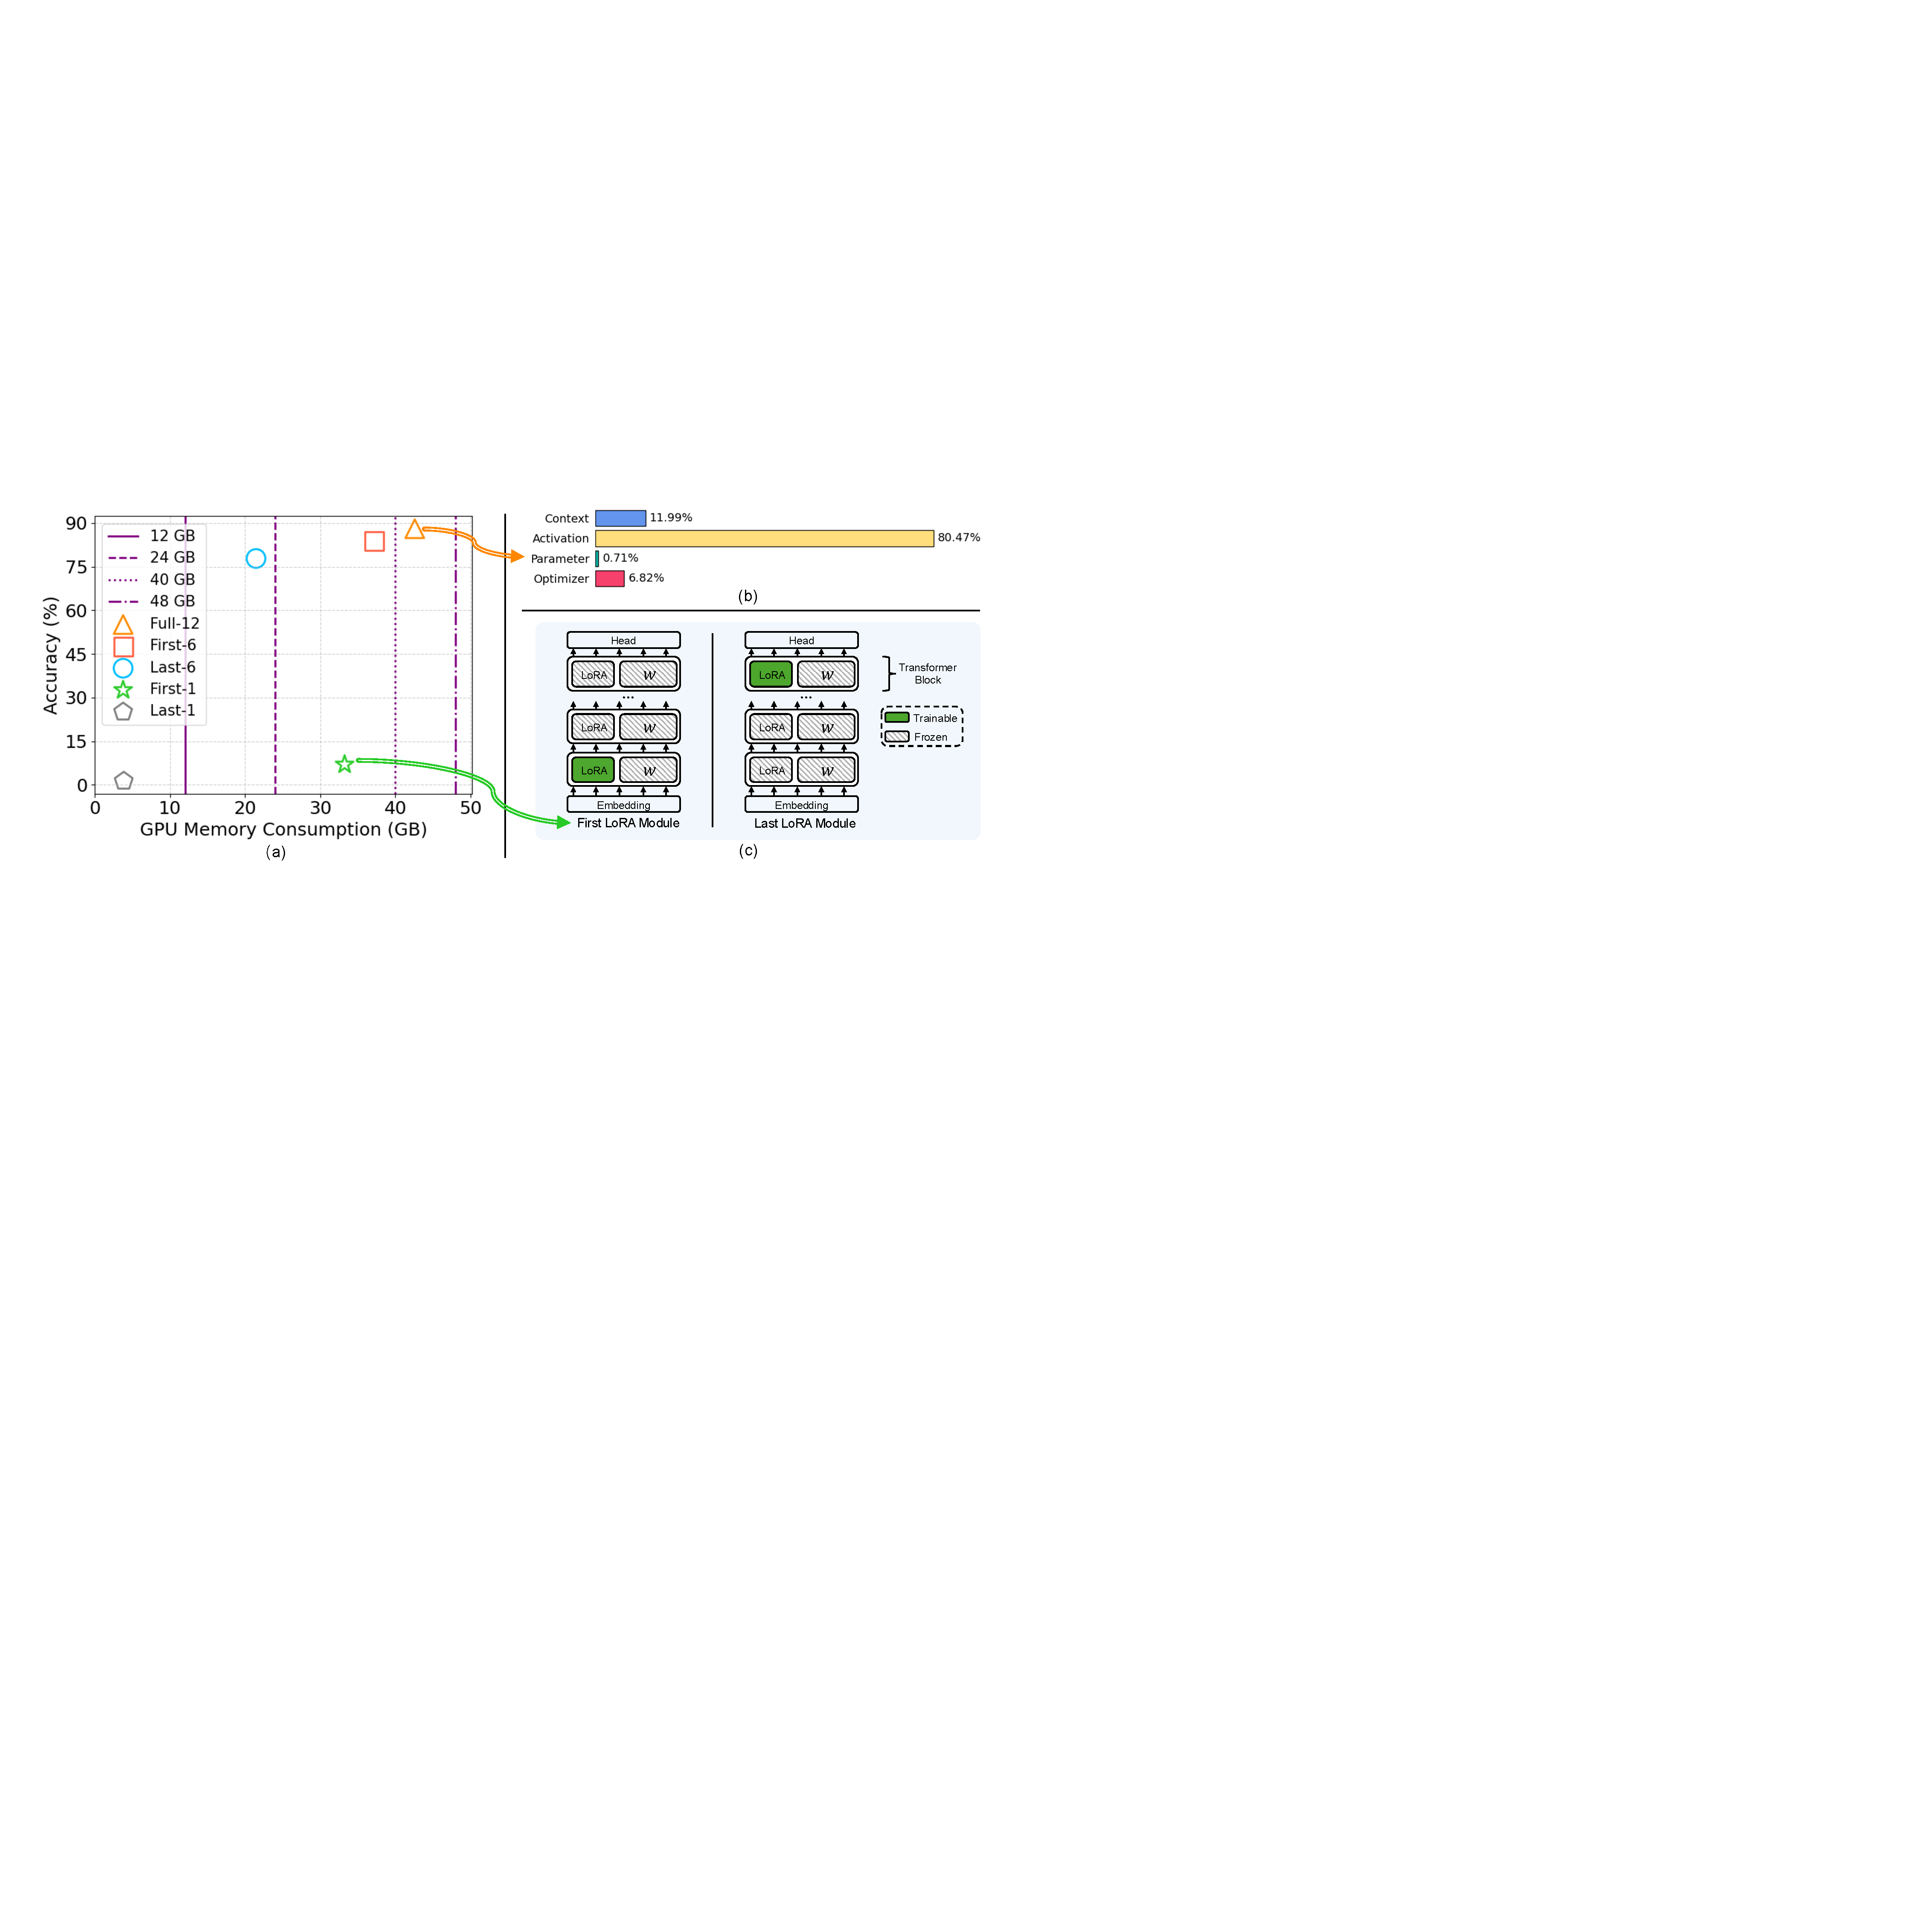
\includegraphics[width=0.48 \textwidth]{fig/motivation.pdf}
% \vspace{-10pt}
% \caption{(a) Model accuracy with respect to GPU memory consumption for different LoRA allocation strategies within the GPU memory capacity bracket. (b) GPU memory consumption for fine-tuning the full-layer ViT-base model with LoRA. (c) Examples of different LoRA allocation strategies.}
% \caption{(a) Different LoRA allocation strategies result in varying GPU memory consumption and fine-tuning accuracy. (b) Activation dominates the largest portion of memory consumption during LoRA-based fine-tuning. (c) The same number of trainable LoRA layers can lead to significant differences in memory consumption. See Supplement~\ref{subsec:appendix-motivation-settings} for experimental details.}
\caption{(a) Accuracy vs. GPU memory consumption for fine-tuning the ViT-base model with trainable LoRA modules at different positions. (b) Breakdown of memory consumption of LoRA fine-tuning. (c) Comparison of training the first LoRA module vs. the last LoRA module while keeping the rest frozen. See {Supplement~\ref{subsec:appendix-motivation-settings}} for experimental details.}
% \caption{Left: GPU Memory Footprint for Fine-Tuning ViT-base~\cite{dosovitskiy2020image} Model. Right: Model Accuracy with Respect to Activation Memory Consumption for Different LoRA Allocation Strategies.}
\label{fig:motivation}
% \vspace{-12pt} 
\end{figure}

% FL first
Federated Learning (FL)~\cite{mcmahan2017communication} enables collaborative model training across distributed edge devices (clients) under the coordination of a central server. In this paradigm, data remains local, and only client-computed model updates are sent to the server to iteratively refine a shared global model. By reducing data collection costs and mitigating privacy risks, FL has emerged as a practical solution for scalable machine learning systems. 
%While FL offers privacy benefits by keeping clients' data locally, it introduces significant challenges in both computational and communication efficiency due to constant model updates and transfers between the server and clients. These challenges are particularly pronounced in resource-constrained edge devices, which operate under limited bandwidth and stringent energy or memory constraints.
% 
% FM
Concurrently, Foundation Models (FMs) have become transformative across various domains due to their large scale and ability to generalize effectively across diverse datasets. These models have driven significant advancements in natural language processing, computer vision, and other fields through task-specific fine-tuning~\cite{touvron2023llama,dosovitskiy2020image}. Recent developments, such as the Llama-family models~\cite{touvron2023llama}, exemplify the rapid expansion of FMs to billions of parameters, showcasing their unprecedented scale and complexity. 
% 
However, the large parameter count of FMs poses significant challenges for deployment in federated settings, as the associated computational and communication overhead severely limits their ability to efficiently utilize distributed data~\cite{su2023fedra}. 

% To address the challenges of deploying FMs in federated settings, we introduce \textbf{Fed-piLot}, a method designed to fine-tune FMs to various downstream tasks in federated environments with significantly reduced computational and communication requirements. Fed-piLot leverages Low-Rank Adaptation (LoRA)~\cite{hu2021lora}, a widely used Parameter-Efficient Fine-Tuning (PEFT)~\cite{lester2021power} approach, as the local training strategy for clients in FL. By training a small set of parameters additive to the pre-trained FM while keeping the rest frozen, LoRA achieves good performance in centralized FM fine-tuning settings, particularly with mid-sized data~\cite{hu2021lora}. Using LoRA locally, clients can fine-tune the FM with low computational cost and communicate updates to the server efficiently.

To address the challenges of deploying FMs in federated settings, Parameter-Efficient Fine-Tuning (PEFT)~\cite{lester2021power} methods have been widely explored. Among these, Low-Rank Adaptation (LoRA) has demonstrated strong performance in efficiently fine-tuning FMs, particularly on mid-sized datasets~\cite{hu2021lora}. 
LoRA achieves this by decomposing weight updates into low-rank matrices, training only these matrices while keeping the pre-trained weights frozen. This approach significantly reduces the number of trainable parameters, lowering both the computational cost of training and the communication overhead for transmitting model updates in FL. 
% By training a small set of parameters added to the pre-trained FM while keeping the rest of the model frozen, clients can achieve efficient fine-tuning with reduced computational and communication costs. 
%
% The widespread adoption of foundation models (FMs)~\cite{dosovitskiy2020image,devlin2019bert} has enhanced the performance and utility of numerous AI-based services. However, building FMs typically requires large volumes of training data, which has traditionally been collected by the service providers. 
% % 
% Federated Learning (FL)~\cite{mcmahan2017communication} addresses this issue by enabling the aggregation of client data without compromising data privacy. 
%
% Integrating FMs into the FL framework has led to the emergence of Federated Foundation Models (FedFMs) as a new learning paradigm. However, fully training FedFMs is resource-intensive and often impractical in the FL setting, particularly in cross-device scenarios. To this end, Parameter-efficient fine-tuning (PEFT) methods~\cite{lester2021power,hu2021lora}, widely explored in centralized FM fine-tuning, offer an effective solution by significantly reducing the number of trainable parameters. Among these, Low-Rank Adaptation (LoRA) has demonstrated strong performance, especially for cases with mid-sized training data~\cite{hu2021lora}.
% 
% Recent research has started exploring the use of LoRA in the context of FL~\cite{zhang2023towards,babakniya2023slora,su2023fedra}. 
Recent studies have explored LoRA's effectiveness in federated fine-tuning~\cite{gao2025flowertune,zhang2025fed,zhang2023towards,cho2024heterogeneous,wangflora,bai2024federated}.
For example, FedIT~\cite{zhang2023towards} proposes a vanilla integration of LoRA and FedAvg~\cite{mcmahan2017communication}, while methods like
%SLoRA~\cite{babakniya2023slora} improves the initialization strategy of LoRA in FL settings. 
% Instead, methods with heterogeneous LoRA ranks for different clients like 
HETLoRA~\cite{cho2024heterogeneous}, FLoRA~\cite{wangflora}, and FlexLoRA~\cite{bai2024federated} adjust LoRA ranks to accommodate clients' varying computational capabilities, optimizing resource usage in heterogeneous settings.
% Rank-based approaches such as HETLoRA~\cite{cho2024heterogeneous}, FLoRA~\cite{wangflora}, and FlexLoRA~\cite{bai2024federated}, employ varying LoRA ranks to accommodate heterogeneous clients.

However, these methods fail to address a critical challenge in fine-tuning FMs in federated settings: the memory bottleneck. Fine-tuning FMs requires substantial on-device GPU memory to store the CUDA context, model parameters, optimizer states, and intermediate activations necessary for gradient computation during back-propagation. Among these, activations dominate memory usage, as illustrated in Figure~\ref{fig:motivation}(b). 
% As illustrated in Figure~\ref{fig:motivation}(b), a GPU memory consumption breakdown for fine-tuning a ViT-base model~\cite{dosovitskiy2020image} (comprising 12 pre-trained transformer blocks with LoRA applied to each block\footnote{Details in Supplement~\ref{subsec:appendix-motivation-settings}}) shows that intermediate activations consume a substantial portion of the memory. 
% 
Although reducing the rank of LoRA modules lowers memory costs associated with optimizer states (e.g., gradients, momentum), it does not significantly alleviate the memory demand for activations.
% 
This memory requirement makes fine-tuning FMs challenging even on powerful GPU servers, let alone on those resource-constrained edge or end devices in federated settings. 
%  Although this can release the computation and communication burden, it does not address the challenges of requiring a significant amount of on-device GPU memory for fine-tune FMs, which in-turn can lead to the computation being inefficient and memory-bounded. 
% 
% Although this reduces computational and communication overhead in FL, it does not alleviate the memory usage during fine-tuning FMs.

Recently, FedRA~\cite{su2023fedra} was proposed to mitigate the memory bottleneck by training only a random subset of LoRA modules on each client, while keeping the remaining modules frozen. However, this approach assumes that freezing any LoRA module results in equal memory savings and overlooks the varying importance of different modules in contributing to model performance, thereby resulting in limited memory efficiency. 
% use the figure to explain the varying memory savings
As shown in Figure~\ref{fig:motivation}(a), training the LoRA modules
% (referred to as LoRA module) 
at different positions (i.e., within different transformer blocks) leads to varying memory consumption and model accuracy. This discrepancy arises because freezing a layer eliminates the storage of dynamic activations, which are associated with linear functions, but does not reduce the memory required for static activations. Static activations, which are generated by non-linear functions, must be stored for gradient computation in subsequent trainable layers (refer to {{Supplement~\ref{sec:appendix-gpu-memory-consumption}}} for details). For example, training the first $u$ LoRA modules requires extra storage for static activations from module $u+1$ onward to compute gradients back to the $u$-th module, even though these modules are frozen. 

% For example, training the first $l$ LoRA layer requires storing the activations for the trainable layers, as well as the static activations from LoRA layers $l$ to 12, even though these layers are frozen. In contrast, training the last $l$ LoRA layer only requires storing activations from the last $l$ LoRA layers.

% For instance, training the first $l$ LoRA layer (e.g., First-1 or First-6), except for all the activations for these trainable layers, it additionally requires the storage of static activations from LoRA layers $l$-12 even though these layers are frozen, while training the last layer (e.g., Last-1 or Last-6) only needs the storage of activations from LoRA layer $l$-12.  

% , which cannot be discarded even when the input layer is frozen due to the non-linearity of functions like GELU, LayerNorm, and Softmax in transformer models. 
% FedRA~\cite{su2023fedra} attempts to mitigate this by randomly selecting a subset of LoRA layers for training on each client. However, this approach assumes equal GPU memory consumption (referred to as memory consumption hereafter) across layers and ignores the varying importance of different layers in contributing to overall performance. 
% due to the storage of intermediate activations for backpropagation\cite{ardakani2024slimfit}. 
% 
% Despite the reduction in computational and communication overhead (i.e., FLOPs) achieved by LoRA's small trainable parameters, a major challenge persists: the high GPU memory consumption on client devices due to storing intermediate data such as activations during training~\cite{ardakani2024slimfit}. 
% This memory burden can prevent low-resource clients from participating in the training process. 
%
%
% To investigate memory consumption and enable FL for heterogeneous clients, we first break down memory consumption into four components, as shown in Figure.~\ref{fig:motivation} (b). When training a ViT-base~\cite{dosovitskiy2020image} model with 12 transformer layers and applying LoRA to each layer\footnote{Refer to experimental details in Supplement~\ref{subsec:appendix-motivation-settings}}, activation memory accounts for the largest share of the total memory consumption. This memory is required to store activations for back-propagation and predominantly resides in the transformer layers.
% FedRA~\cite{su2023fedra} attempts to mitigate this issue by randomly selecting a subset of LoRA layers for training on each client. However, this approach assumes equal memory consumption across layers and overlooks the varying importance of different layers to overall performance. 
% 
% Intuitively, we adopt a layer-wise freezing strategy for federated FM (FedFM) fine-tuning for heterogeneous clients and compare the overall memory consumption and global model performance for each strategy. Specifically, we conduct experiments by training the first 1, first 6, last 1, last 6, and all 12 LoRA layers on the CIFAR-100 dataset, as shown in Figure.~\ref{fig:motivation} (a). These strategies lead to varying memory consumption, which corresponds to different memory capacity brackets commonly seen in real-world NVIDIA GPUs\footnote{NVIDIA RTX A2000: 12GB, NVIDIA RTX A5000: 24GB, NVIDIA Tesla A100: 40GB, NVIDIA RTX A6000: 48GB.}. 
% 
% Due to the presence of static activations~\cite{ardakani2024slimfit}, which cannot be discarded because of non-linear functions (e.g., GELU, LayerNorm, and Softmax), the memory consumption for training the first 1 or 6 layers approaches that of training all 12 layers. Additionally, the results reveal a notable performance disparity based on which LoRA layers are trained (e.g., a comparison between the ``Last 6'' and ``First 6'' strategies), highlighting the varying importance of different layers in the model. Therefore, a research question naturally arises:

% \textit{How to optimize LoRA layer allocation within a client's memory capacity bracket (the vertical lines in Figure.~\ref{fig:motivation} (a)) to maximize global model performance?}

In this work, we introduce \textbf{Fed-pilot}, a novel memory-efficient method for \textbf{\uline{fed}}erated fine-tuning of FMs across clients with heterogeneous memory capacities. Fed-pilot identifies the o\textbf{\uline{p}}t\textbf{\uline{i}}mal al\textbf{\uline{lo}}ca\textbf{\uline{t}}ion of local trainable LoRA modules that maximize global model performance under memory constraints. To aggregate local LoRA updates, Fed-pilot introduces a compensated aggregation rule, which mitigates the inconsistencies across layers caused by Non-IID data distributions and heterogeneous LoRA allocation to ensure model convergence.
% 
% Based on these findings, we introduce \textbf{Fed-piLot}, an efficient \uline{\textbf{Fed}}FM fine-tuning framework that o\uline{\textbf{p}}t\uline{\textbf{i}}mizes trainable \uline{\textbf{Lo}}RA layer alloca\uline{\textbf{t}}ion for clients with heterogeneous memory constraints. 
% 
% In this framework, we formulate the LoRA allocation as a knapsack optimization problem, where the objective is to maximize global model performance while adhering to memory capacity limits. 
%
% To achieve this, we design a dynamic \textit{weight} function by calculating GPU memory consumption for training different LoRA layers. For the \textit{value} function, we propose an Information Gain Score (IG-Score), which quantifies the importance of each layer by integrating both local and global information during training. 
%
% To address the challenge of diverging local model updates caused by the optimized LoRA allocation and Non-IID data distribution, we introduce a Historical Model Update Aggregation (HAgg) rule. This approach enhances the robustness of the global model by mitigating the influence of misleading updates from a minority of clients and leveraging historical information from model updates to improve overall performance. 
% 
Our main contributions are summarized as follows:

\begin{itemize}
    \item We propose Fed-pilot, a novel federated LoRA-based fine-tuning framework designed for clients with heterogeneous memory constraints. Fed-pilot enables clients with limited memory to dynamically train an optimal subset of LoRA modules, which can effectively reduce memory requirements during fine-tuning. 
    % For optimization, we model the non-linear relationship between LoRA allocation and memory consumption, considering both dynamic and static activations. 
    To the best of our knowledge, this is the first study on federated fine-tuning of FMs that incorporates memory-constrained optimization. %practical memory consumption modeling.
    \item We formulate the allocation of trainable LoRA modules as a knapsack optimization problem, aiming to maximize the fine-tuning performance under memory constraints. We model the GPU memory consumption of LoRA-based fine-tuning, including scenarios with partial LoRA allocation. We design an information gain (IG) score based value function to quantify the LoRA module's contribution to model performance from local and global perspectives. 
    
    % By incorporating client-specific information, the IG score adapts to local data distributions.
    % the For the value function, we introduce an IG-Score that quantifies each layer's contribution to performance. By incorporating client-specific information, IG-Score adapts to various data distributions. 
    \item In addition, we design a novel aggregation rule ComAgg to mitigate the significant divergence among local model updates caused by heterogeneous LoRA allocation and Non-IID data.
    \item We conduct extensive experiments using five datasets in IID and various Non-IID settings and compare Fed-pilot with state-of-the-art methods to demonstrate its effectiveness and efficiency.
\end{itemize}

% The rest of the paper is organized as follows: In Section~\ref{relatedwork}, we review related works, followed by the system modeling in Section~\ref{sec:sys_model}. In Section~\ref{framework}, we introduce the development of our Fed-piLot framework. Next, we evaluate our approach through numerical experiments in Section~\ref{evaluation}. Finally, we conclude the paper in Section~\ref{conclusion}.


\section{Related Work}\label{relatedwork}

\textbf{LoRA-based Federated Fine-Tuning.} FL has been applied to the PEFT of FMs, enabling multiple clients to collaboratively fine-tune FMs without sharing their data~\cite{zhang2023towards,babakniya2023slora,sun2024improving}.
There is growing interest in LoRA-based federated fine-tuning approaches, which are commonly known to be particularly effective in mid-sized data scenarios~\cite{hu2021lora}. 
FedIT~\cite{zhang2023towards} proposes a vanilla federated fine-tuning method with LoRA and establishes benchmarks for PEFT in FL. SLoRA~\cite{babakniya2023slora} is a two-stage approach that trains local models with sparse fine-tuning for several rounds and then switches to LoRA for PEFT. FFA-LoRA~\cite{sun2024improving} enhances the privacy of federated fine-tuning using differential privacy. {FedSA-LoRA}~\cite{guo2024selective} only shares the A matrices with the server for aggregation, due to their specific role in learning general knowledge. However, these methods assume homogeneous client resources.


\textbf{Federated Fine-Tuning under Heterogeneous Clients.} While LoRA-based federated fine-tuning methods can save computational and communication costs, they still fail to fully accommodate training across heterogeneous clients with varying memory capacities. A range of rank-based methods~\cite{cho2024heterogeneous,wangflora,bai2024federated} attempt to address this by assigning different LoRA ranks according to clients' memory capacities.
% HETLoRA~\cite{cho2024heterogeneous} proposes a heterogeneous LoRA rank strategy and adapts FedAvg for aggregation with the first few shared LoRA ranks.
% HETLoRA~\cite{cho2024heterogeneous} introduces a heterogeneous LoRA rank strategy, where clients train different numbers of LoRA ranks based on their memory capacity. Aggregation follows a hierarchical approach, averaging only the ranks shared by multiple clients while higher ranks, trained by fewer clients, contribute selectively
HETLoRA~\cite{cho2024heterogeneous} introduces a heterogeneous LoRA rank strategy, where clients train different numbers of LoRA ranks based on their memory capacity. Its aggregation rule follows a hierarchical approach, ranks shared by multiple clients are averaged, while higher ranks are aggregated by fewer clients.
FLoRA~\cite{wangflora} introduces a stacking method for all LoRA ranks to mitigate the aggregation noise from aggregating low-rank compositions separately. FlexLoRA~\cite{bai2024federated} utilizes singular value decomposition (SVD) to redistribute attention weight matrix for clients with varying ranks. However, reducing the LoRA rank does not result in significant memory reduction, making it an inefficient solution for memory-constrained settings.
FedRA~\cite{su2023fedra} proposes a layer-wise LoRA allocation strategy that randomly selects partial LoRA modules each round to handle resource disparities among clients. However, it fails to account for the non-linear nature of memory consumption and the varying impact of different layers on overall global model performance.
% FedRA~\cite{su2023fedra} introduces a layer-wise LoRA allocation method that randomly select partial LoRA modules each round to address resource disparities among clients but overlooks the non-linear nature of memory consumption and the varying contributions of layers to overall model performance.
% FedRA~\cite{su2023fedra} introduces layer-wise LoRA allocation for clients with varying resources but neglects the non-linear GPU memory consumption and differing layer contributions to model performance. 
A well-designed heterogeneous LoRA allocation is essential for achieving optimal performance in federated fine-tuning systems with memory constraints. % Refer to Section~\ref{sec:appendix-comparative_study} in Supplement for a comparative study of these related works.

\textbf{Layer Freezing for Training Efficiency.} 
{
Layer freezing has been used to improve the training efficiency of FMs}~\cite{pan2024lisa,zhu2023lift,yao2024layer}.
LISA~\cite{pan2024lisa} randomly selects a subset of layers to fine-tune in each training step, thereby reducing the number of trainable parameters. LIFT~\cite{zhu2023lift} fine-tunes only one FM layer per step and applies different selection strategies throughout training, leading to reduced computational costs. IST~\cite{yao2024layer} introduces a reinforcement learning-based method to select a subset of layers during fine-tuning. Other methods in FL~\cite{liu2024fisher,wu2024fedfmsl} also incorporate layer freezing to improve training efficiency. 
FibecFed~\cite{liu2024fisher} designed a Fisher Information Matrix-based scoring mechanism to selectively fine-tune a subset of LoRA modules for each client.
FedFMSL~\cite{wu2024fedfmsl} progressively unfreezes LoRA modules from higher to shallow layers for efficient training, relying on heuristic training-time accuracy gains to determine when to unfreeze more LoRA modules.
However, these methods do not account for practical memory modeling, particularly the non-linear activation memory reduction by layer freezing. Our method optimizes LoRA allocation under memory constraints while preserving the global model performance.


\section{System Modeling}\label{sec:sys_model}

% \begin{figure}[t]
% \centering
% 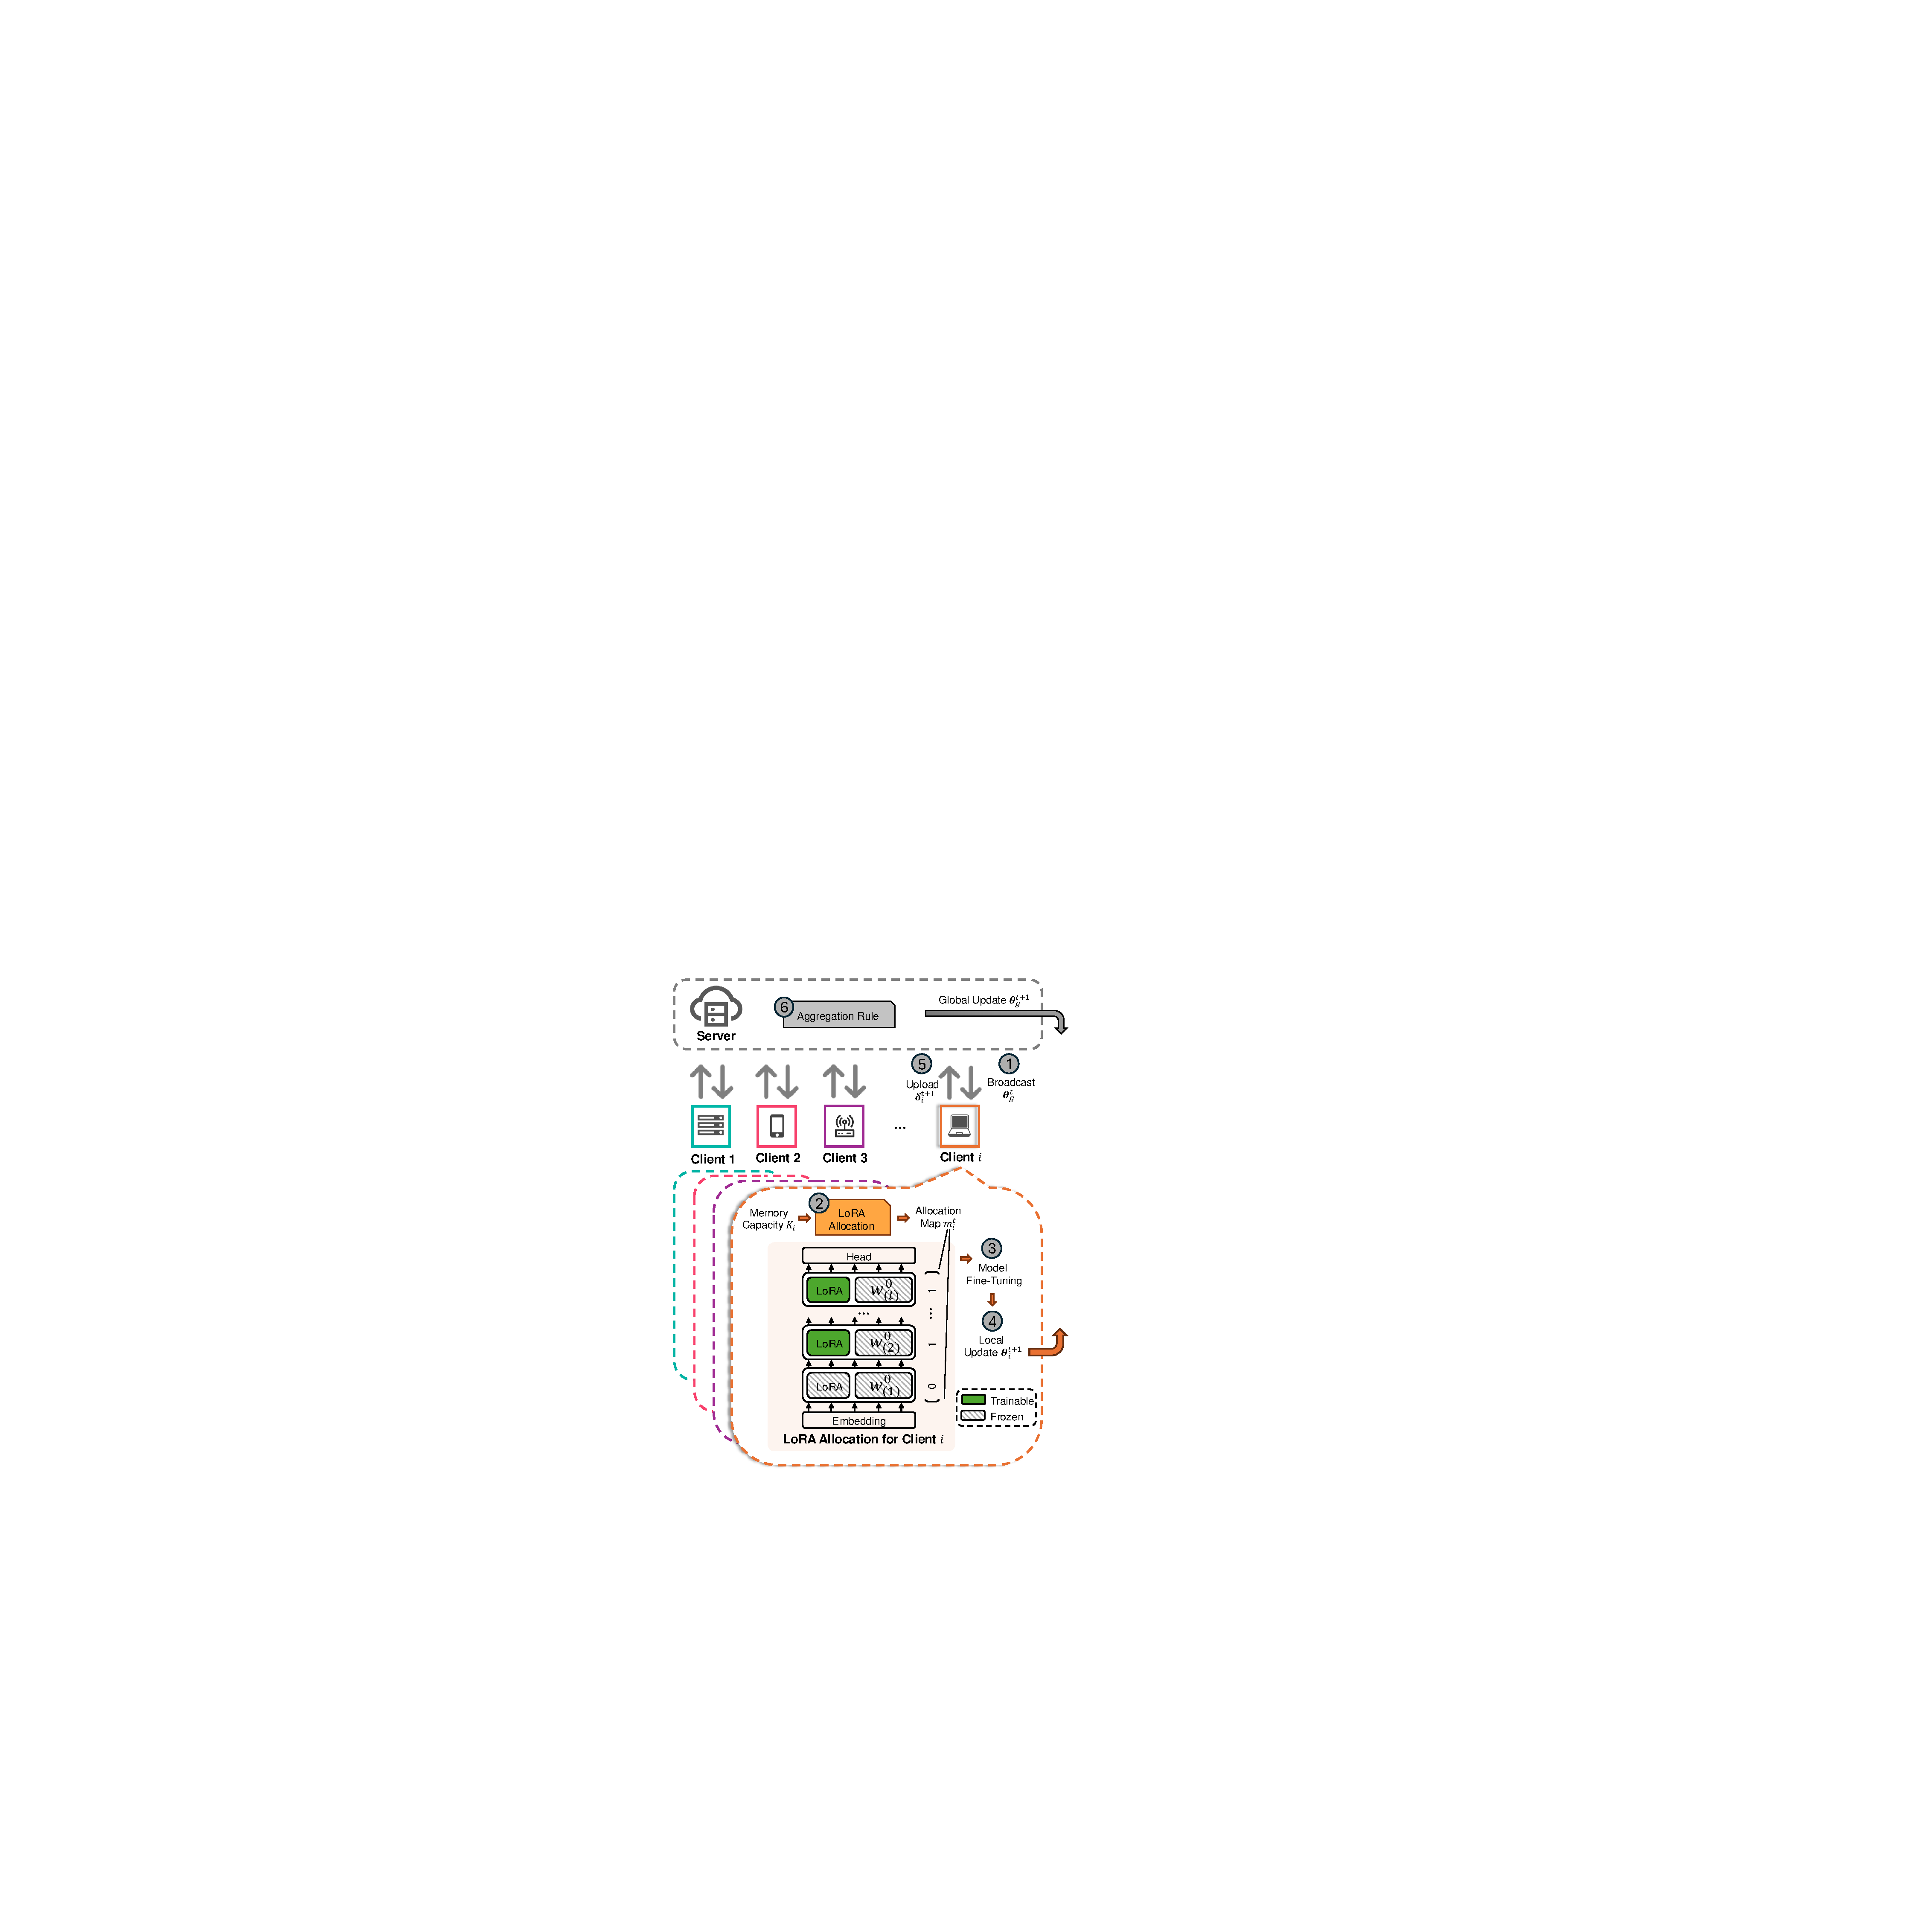
\includegraphics[width=0.40\textwidth]{fig/overallFramework.pdf}
% % \vspace{-10pt}
% \caption{The overall system of Federated Fine-Tuning with heterogeneous clients.}
% \label{fig:framework}
% \vspace{-12pt} 
% \end{figure}

\subsection{Federated Fine-Tuning System}\label{sec:leaning_model}
We consider a federated fine-tuning system consisting of a central server and $v$ clients. The server has a global FM $\boldsymbol{\Theta}$ initialized with pre-trained weights $\boldsymbol{\Theta}^0$. Each client $i\in[v]$ owns a local dataset $D_i\sim\mathcal{P}_i$, where the size of $D_i$ and the data distribution $\mathcal{P}_i$ can vary across clients. In federated fine-tuning, clients aim to collaboratively fine-tune the global model $\boldsymbol{\Theta}$ under the coordination of the server.

% We consider a Federated Fine-Tuning system, the system consists of a central server and multiple clients, the global FM $\boldsymbol{\Theta}$ initialized with pre-trained weights $\boldsymbol{\Theta}^0$ on the server, and collaborative fine-tuned by $v$ clients over multiple rounds. 
In this work, we focus on transformer-based models~\cite{touvron2023llama,zhang2022opt,devlin2019bert,dosovitskiy2020image} consisting of $l$ transformer blocks $\{\boldsymbol{\mathcal{W}}_{(1)}, \cdots, \boldsymbol{\mathcal{W}}_{(l)}\}$, and embedding layers, along with head layers, denoted as $\boldsymbol{\mathcal{W}}_{rest}$. The pre-trained model is thus represented as $\boldsymbol{\Theta}^0=\{\boldsymbol{\mathcal{W}}_{(1)}^0, \cdots, \boldsymbol{\mathcal{W}}_{(l)}^0, \boldsymbol{\mathcal{W}}_{rest}^0\}$. 
% 
To fine-tune the global model efficiently, we apply the LoRA module (denoted as $\boldsymbol{\theta}_{(j)}$) to the attention weight $\boldsymbol{\mathcal{A}}_{(j)}\in\mathbb{R}^{d \times k}$ within the $j$-th transformer block, where $j\in[1,l]$, and $d$ and $k$ represent the dimensions of the input and output feature space of attention layers, respectively. 
%
The idea behind LoRA is to constrain $\Delta\boldsymbol{\mathcal{A}}_{(j)}$, the update of a pre-trained attention weight matrix $\boldsymbol{\mathcal{A}}_{(j)}^0$, using a low-rank decomposition, such that $\boldsymbol{\mathcal{A}}_{(j)}^0 + \Delta\boldsymbol{\mathcal{A}}_{(j)}=\boldsymbol{\mathcal{A}}_{(j)}^0+\boldsymbol{\mathcal{N}}_{(j)}\boldsymbol{\mathcal{M}}_{(j)}$, where $\boldsymbol{\mathcal{N}}_{(j)}\in\mathbb{R}^{d \times r}$, $\boldsymbol{\mathcal{M}}_{(j)}\in\mathbb{R}^{r \times k}$, and the rank $r \ll \min(d, k)$. Without loss of generality for subsequent optimization, we omit $\boldsymbol{\mathcal{W}}_{rest}$ and define the LoRA modules for $\boldsymbol{\Theta}$ 
% \hl{as $\boldsymbol{\theta} := \{\Delta\boldsymbol{\mathcal{A}}_{(1)}, \cdots, \Delta\boldsymbol{\mathcal{A}}_{(l)}\}$. vs 
as $\boldsymbol{\theta} := \{ \boldsymbol{\theta}_{(j)}\}_{j\in[l]}$ with $\boldsymbol{\theta}_{(j)} = \{\boldsymbol{\mathcal{N}}_{(j)},\boldsymbol{\mathcal{M}}_{(j)}\}$.
% Each client $i\in[v]$ collects a dataset $D_i\sim\mathcal{P}_i$, where the amount of $D_i$ and the data distribution $\mathcal{P}_i$ can vary across clients. 

%
In this context, the problem of federated fine-tuning using LoRA can be formulated as follows:
\begin{equation}\label{eq:ffm_obj}
\min_{\boldsymbol{\mathcal{\theta}}} \mathcal{L}(\boldsymbol{\mathcal{\theta}}) := \frac{1}{v}\sum_{i=1}^{v} \mathcal{L}_{i}(\boldsymbol{\mathcal{\theta}}; \boldsymbol{\Theta}^0),
\end{equation}
where $\mathcal{L}_{i}(\boldsymbol{\mathcal{\theta}}; \boldsymbol{\Theta}^0) := \mathbb{E}_{x \in  D_i}[\ell(\boldsymbol{\mathcal{\theta}};\boldsymbol{\Theta}^0,x)]$ denotes the local objective function of client $i$, and $\ell(\boldsymbol{\mathcal{\theta}}_i;\boldsymbol{\Theta}^0,x)$ is the loss of the model $\{\boldsymbol{\mathcal{\theta}}, \boldsymbol{\Theta}^0 \}$ on a datapoint $x$ sampled from ${D}_i$. 
% 
We assume that clients download the pre-trained weights $\boldsymbol{\Theta}^0$ from the server prior to fine-tuning and have sufficient memory capacity to store the model parameters. Ideally, the classic FedAvg algorithm~\cite{mcmahan2017communication} can be employed to solve this problem in a distributed manner. In FedAvg, at round $t$, clients download the global trainable model parameters $\boldsymbol{\mathcal{\theta}}^t$ maintained by the server and update it using their local datasets to minimize their local objectives. Clients then upload their model updates to the server, which aggregates the updates to compute $\boldsymbol{\mathcal{\theta}}^{t+1}$ for the next round of fine-tuning. 
% 
However, in practice, the large memory requirements for fine-tuning FMs, coupled with the heterogeneity of clients' memory capacities, prevent some clients from accommodating the memory cost necessary for locally optimizing $\boldsymbol{\mathcal{\theta}}$. %In the following, we model the on-device GPU memory consumption during the fine-tuning process. 

% To address the problem, at each round $t\in[T]$, the server broadcasts the current global trainable parameters $\boldsymbol{\mathcal{\theta}}_g^t$ to a subset of $q$ clients, denoted as $\mathbb{Q}^t$. Each client initializes its local model $\boldsymbol{\Theta}_i^t=\{\boldsymbol{\mathcal{\theta}}_i^t; \boldsymbol{\Theta}^0 \}$ using the global parameters $\boldsymbol{\mathcal{\theta}}_g^t$, such that $\boldsymbol{\Theta}_i^t=\{\boldsymbol{\mathcal{\theta}}_g^t; \boldsymbol{\Theta}^0 \}$. After fine-tuning $\boldsymbol{\Theta}_i^t$ using its local dataset $D_i$, the updated parameters $\boldsymbol{\mathcal{\theta}}_i^{t+1}$ are obtained. Each client then uploads the local update $ \boldsymbol{\delta}_i^{t+1} := \boldsymbol{\mathcal{\theta}}_i^{t+1} - \boldsymbol{\mathcal{\theta}}_i^t$ to the server. The server updates the global trainable parameters by computing
% $\boldsymbol{\mathcal{\theta}}_g^{t+1} := \boldsymbol{\mathcal{\theta}}_g^t + ({1}/{q})\sum_{i\in \mathbb{Q}^t}\boldsymbol{\delta}_i^{t+1},$ which results in the global model $\boldsymbol{\Theta}_g^{t+1}=\{\boldsymbol{\mathcal{\theta}}_g^{t+1};\boldsymbol{\Theta}^0\}$ for the next training round. The process continues until the global model converges.

% While the ordinary federated fine-tuning framework assumes homogeneity across clients, in real-world scenarios, clients often operate under heterogeneous conditions, such as varying memory capacities. This adds complexity to the optimization problem, as not all clients can train the full set of LoRA layers $\boldsymbol{\mathcal{\theta}}_i$, making it necessary to account for memory capacities when allocating trainable parameters. 

% To address these variations in memory capacities, the following subsections detail the process of memory consumption modeling, explain how LoRA allocation impacts memory consumption, followed by two special cases, and finally reformulate the federated fine-tuning problem with LoRA allocation while presenting our proposed solution.

\subsection{On-Device GPU Memory Consumption of LoRA-based Fine-Tuning}\label{sec:memory_consumption}
FM fine-tuning requires substantial on-device GPU memory, primarily due to the complexity of the transformer model architecture. In federated settings with memory-limited clients, understanding the memory footprint of a FM fine-tuning task is crucial for designing memory-efficient approaches. 
% 
% We present a comprehensive model of memory consumption for transformer-based FM. 
% The total memory consumption denoted as $\mathcal{C}_{total}$, which accounts for the primary factors in the LoRA-based fine-tuning process: model parameters $\mathcal{C}_p$, optimizer states $\mathcal{C}_o$, activations $\mathcal{C}_a$, and the CUDA context $\mathcal{C}_c$. 
% 
Let $\mathcal{C}$ denotes the total memory consumption for a LoRA-based FM fine-tuning process. It can be represented as $\mathcal{C}=\mathcal{C}_p+\mathcal{C}_o+\mathcal{C}_a+\mathcal{C}_c$, where $\mathcal{C}_p$, $\mathcal{C}_o$, $\mathcal{C}_a$ and $\mathcal{C}_c$ represent the memory consumption of model parameters, optimizers, activations and the CUDA context, respectively.

(1) Model parameters include all weights and biases used during fine-tuning, encompassing both trainable and frozen parameters. Based on the federated fine-tuning problem formulation in~\eqref{eq:ffm_obj}, 
% the memory consumption for storing model parameters in bytes can be expressed as $\mathcal{C}_p:=\varphi(\{\boldsymbol{\theta}; \boldsymbol{\Theta}^0\})=\eta N_{weight}(\{\boldsymbol{\theta}; \boldsymbol{\Theta}^0\})+\eta N_{bias}(\{\boldsymbol{\theta}; \boldsymbol{\Theta}^0\})$ where $N_{weight}(\cdot)$ and $N_{bias}(\cdot)$ are the number of weights and bias in the model, and $\eta$ is the number of bytes used required by the datatype of parameters (e.g., 2 bytes for 16-bit precision).
the memory consumption for storing model parameters in bytes can be expressed as $\mathcal{C}_p:=\varphi(\{\boldsymbol{\theta}, \boldsymbol{\Theta}^0\}) $ where $ \varphi$ is defined as $\varphi(\boldsymbol{z}) =\eta N_{weight}(\boldsymbol{z})+\eta N_{bias}(\boldsymbol{z})$. Here, $N_{weight}(\cdot)$ and $N_{bias}(\cdot)$ are the number of weights and bias in the model $\boldsymbol{z}$, and $\eta$ is the number of bytes per parameter, which is determined by the precision (e.g., 2 bytes for 16-bit precision). 
% Although memory consumption from model parameters is notable, it is relatively insignificant compared to activations, as shown in Figure~\ref{fig:motivation}. 

(2) Modern gradient-based optimizers like Adam~\cite{kingma2014adam} are widely used in FM fine-tuning. They maintain state information such as first-order and second-order gradient estimates for each trainable parameter. 
%In the LoRA-based fine-tuning model, the number of trainable parameters is significantly reduced. 
Consequently, the memory consumption for optimizer states scales linearly with the number of trainable model parameters and can be approximated as $\mathcal{C}_o:=b\zeta\varphi(\boldsymbol{\theta})$, where $\zeta$ represents the number of optimizer states and $b$ is the batch size.

(3) %During fine-tuning, activations are computed and stored for backpropagation. 
Unlike optimizer states, activation memory in transformer model fine-tuning grows non-linearly with the number of trainable parameters~\cite{ardakani2024slimfit}. We distinguish between dynamic activations, which can be discarded by freezing certain parameters, and static activations, retained due to non-linear functions like GELU, LayerNorm, and Softmax (see {{Supplement~\ref{subsec:appendix-dynamic-activation}-\ref{subsec:appendix-memory-footprint-example}}} for details). We calculate the size of dynamic and static activations for each transformer block in $\{\boldsymbol{\mathcal{\theta}}, \boldsymbol{\Theta}^0\}$, when pre-trained weights $\boldsymbol{\Theta}^0$ are frozen and the LoRA modules $\boldsymbol{\mathcal{\theta}}$ are trainable. As a result, the memory consumption for storing activations during the update of $\boldsymbol{\mathcal{\theta}}$ is given by: $\mathcal{C}_a:=b\eta{\textstyle \sum_{j=1}^{l}}\sigma_{(j)}^d + b\eta{\textstyle \sum_{j=1}^{l}}\sigma_{(j)}^s$, where $\sigma_{(j)}^d$ and $\sigma_{(j)}^s$ represents the size of dynamic and static activations for the $j$-th block.
%We categorize the activations into two types: dynamic and static. {Dynamic activations can be discarded by freezing training parameters, while static activations cannot be discarded by block freezing due to the presence of non-linear functions (e.g., GELU, LayerNorm, and Softmax, we provide detailed explanations in Supplement~\ref{subsec:appendix-dynamic-activation}-\ref{subsec:appendix-memory-footprint-example}).} 
% The total memory consumption for storing activations for all the blocks is given by: $\mathcal{C}_a:=b\eta{\textstyle \sum_{j=1}^{l}}\sigma_{d}(\boldsymbol{\mathcal{W}}_{(j)}) + b\eta{\textstyle \sum_{j=1}^{l}}\sigma_{s}(\boldsymbol{\mathcal{W}}_{(j)})$, where $\sigma_{d}(\cdot)$ and $\sigma_{s}(\cdot)$ count the size of dynamic and static activations, respectively.

(4) Finally, the memory consumption of the CUDA context includes GPU kernel launches, memory management, and other operational resources. 
% This component is typically model-independent and represents a fixed overhead that varies based on the GPU model and configuration, 
This component highly depends on the environment, machine, and configuration, thus, we treat $\mathcal{C}_c$ as a constant. Overall, the total memory consumption $\mathcal{C}$ is formulated as, 
\begin{equation}\label{eq:memory_model}
\begin{aligned}
\mathcal{C} = & \ \varphi(\{\boldsymbol{\theta}, \boldsymbol{\Theta}^0\}) + b\zeta\varphi(\boldsymbol{\theta}) + b\eta{\textstyle \sum_{j=1}^{l}}\sigma_{(j)}^d  \\
& + b\eta{\textstyle \sum_{j=1}^{l}}\sigma_{(j)}^s
 + \mathcal{C}_c.
\end{aligned}
\end{equation}
This indicates that reducing the size of $\boldsymbol{\theta}$ can further lower the memory cost, similar to existing methods~\cite{cho2024heterogeneous,wangflora,bai2024federated} that reduce the ranks of LoRA modules to save memory cost. However, this saving is limited. As shown in Figure.\ref{fig:motivation}(b), the overall memory cost is primarily dominated by activations. Reducing the ranks of LoRA modules has a minimal impact on the size of both dynamic and static activations. 
% \begin{equation}\label{eq:memory_model}
% \begin{aligned}
% \mathcal{C}_{\text{total}} = & \ \varphi(\{\boldsymbol{\theta}; \boldsymbol{\Theta}^0\}) + b\zeta\varphi(\boldsymbol{\theta})  + {\textstyle b\eta\sum_{j=1}^{l}} \sigma_{d}(\boldsymbol{\mathcal{W}}_{(j)}) \\
% & + {\textstyle b\eta\sum_{j=1}^{l}} \sigma_{s}(\boldsymbol{\mathcal{W}}_{(j)}) 
%  + \mathcal{C}_c.
% \end{aligned}
% \end{equation}
% From Fig.~\ref{fig:motivation}, we can see that activations occupy the largest share of the total memory footprint. From Equation~\eqref{eq:memory_model}, we find that less active transformer layers leads to lower memory consumption for activations. Hence, we prone to layer freezing to save the activation memory footprint.

% From Fig.~\ref{fig:motivation}, we observe that activations account for the largest portion of the total memory footprint. Equation\eqref{eq:memory_model} shows that reducing the number of active transformer layers decreases memory consumption for activations. Therefore, we adopt layer freezing to reduce the memory footprint of activations in the following section.

% From Figure.\ref{fig:motivation}(b), we observe that activations dominate the total memory footprint. In~\eqref{eq:memory_model}, we also find that reducing the number of active transformer blocks effectively lowers memory consumption for activations. 
% Therefore, in the following section, we implement LoRA allocation to reduce the activation memory consumption by freezing some LoRA layers.

% \begin{figure}[t]
% \centering
% \includegraphics[width=0.39\textwidth]{fig/overallFramework.png}
% % \vspace{-10pt}
% \caption{The Overall Framework of Federated Fine-Tuning with Heterogeneous Clients.}
% \label{fig:framework}
% % \vspace{-12pt} 
% \end{figure}

\subsection{Reducing Memory Consumption with Partial LoRA Allocation}\label{subsec:lora-allocation}
%
% Federated Fine-Tuning involves substantial memory consumption, which is not feasible for every client. 
% As discussed earlier, activation memory constitutes the majority of overall memory consumption during the fine-tuning process. To enable efficient Federated Fine-Tuning, we propose LoRA allocation in our framework, allowing memory-limited clients to train only a subset of LoRA layers, constrained by their memory capacity.
%

To save GPU memory consumption, the primary contributor—activation memory cost—should be reduced. 
%
In fact, we can eliminate the need to store the dynamic activations for a transformer block by freezing its LoRA modules, as the entire block is frozen in this case. This is why FedRA~\cite{su2023fedra}, which randomly freezes LoRA modules in some transformer blocks, can reduce certain activation memory consumption. However, previous works do not clearly model the impact of freezing LoRA modules on overall memory cost reduction. 

Let $m:=\{m_{(1)}, m_{(2)}, \cdots, m_{(l)}\}$ represent the LoRA allocation map for the model $\{\boldsymbol{\mathcal{\theta}}, \boldsymbol{\Theta}^0\}$, where $m_{{(j)}}=1$ if the LoRA module in $j$-th block, i.e., $\boldsymbol{\mathcal{\theta}}_{(j)}$, is trainable, otherwise $m_{{(j)}}=0$ if it is frozen. Let $\mathcal{J} = \{ j \mid m_{(j)} = 1,\forall j\}$, the overall memory computation with partial LoRA allocation should be: 
\begin{equation}\label{eq:memory_model2}
    \mathcal{C}(m)=\mathcal{C}_p +\mathcal{C}_o (m) +\mathcal{C}_a (m)+\mathcal{C}_c, 
\end{equation} where $\mathcal{C}_{o} (m) =  b\zeta \varphi(\{\boldsymbol{\mathcal{\theta}}_{(j)}\}_{j\in\mathcal
J})$ and
\begin{equation}\label{eqn:ca}
\mathcal{C}_{a} (m) = b\eta\sum_{j \in \mathcal{J}} \sigma_{(j)}^{d}
 + {b\eta\sum_{j=\min(\mathcal{J})
}^{l}} \sigma_{(j)}^{s}. 
\end{equation}
Freezing LoRA modules affects only the memory cost of optimizer states and activations. The memory consumption of dynamic activations (the first term in \eqref{eqn:ca}) is associated only with trainable LoRA modules. The memory consumption of static activations (the second term in \eqref{eqn:ca}) depends on the earliest trainable LoRA modules, i.e., $\min(\mathcal{J})$, since static activations from all layers after $\min(\mathcal{J})$-th layer must be stored for backpropagation~\cite{ardakani2024slimfit}. This formulation indicates that, in addition to reducing memory usage for optimizer states and dynamic activations, partial LoRA allocation has the potential to reduce the memory usage for static activations, though it must be carefully designed. In the following, we discuss two naive allocation strategies and analyze their memory consumption. 

\textit{Two Naive Cases: Memory Saver and Memory Hogger.} 
% Here, we illustrate two special cases to demonstrate how different LoRA allocations impact memory consumption. 
Memory Saver makes the last $u$ LoRA modules trainable, resulting in the LoRA allocation map is $m_{\text{MS}}= \{0 \ \text{for} \ j \in [1, l-u], \ 1 \ \text{for} \ j \in [l-u+1, l]\}$. Memory Hogger makes the first $u$ LoRA modules trainable, yielding the LoRA allocation map $m_{\text{MH}}= \{1 \ \text{for} \ j \in [1, u], \ 0 \ \text{for} \ j \in [u+1, l]\}$. Despite both having the same number of trainable LoRA modules, these strategies differ in their memory-saving capabilities, particularly in reducing static activation memory, as $\mathcal{C}_{\text{MH}}-\mathcal{C}_{\text{MS}}={b\eta\sum_{j=1
}^{l-u}} \sigma_{(j)}^{s}$, which can be substantial as demonstrated in Figure~\ref{fig:motivation}(a).

% Special Case \circled{2}: Memory Hogger designs the LoRA allocation map as $m_{\text{MH}}= \{1 \ \text{for} \ j \in [1, u], \ 0 \ \text{for} \ j \in [u+1, l]\}$, where the first $u$ LoRA layers are fine-tuned. Despite having the same number of trainable LoRA layers, the memory consumption difference between these two cases is $\mathcal{C}_{\text{MH}}-\mathcal{C}_{\text{MS}}={b\eta\sum_{j=1
% }^{l-u}} \sigma_{s}(\boldsymbol{\mathcal{W}}_{(j)})$, which can be substantial as shown in Figure~\ref{fig:motivation}(a).

% was proposed to mitigate the memory bottleneck by training only a random subset of LoRA layers on each client, while keeping the remaining layers frozen.

% To account for heterogeneous clients, we define the memory capacity for each client $i$ as $\mathcal{K}_i$, where $\{\mathcal{K}_1, \mathcal{K}_2, \dots, \mathcal{K}_v\}$ represents the capacities of all clients, with $v$ being the total number of clients, allowing for differences in memory capacity among them. Based on our analysis of the memory consumption of LoRA-based fine-tuning in Section~\ref{sec:memory_consumption}, reducing the number of active transformer blocks (i.e., trainable LoRA layers within each block) can significantly lower memory consumption for optimizers and activations. Specifically, assume that each client $i$ has a LoRA allocation map
% % 
% % In round $t$, we define an allocation map 
% $m_i^t:=\{m_{i,(1)}^t, m_{i,(2)}^t, \cdots, m_{i,(l)}^t\}$
% % for each client $i$, 
% in round $t$, representing the trainable status of each local LoRA layer in $\boldsymbol{\theta}_i^t$. Here, $m_{i,{(j)}}^t=1$ if the $j$-th LoRA layer is trainable, otherwise $m_{i,{(j)}}^t=0$ if it is frozen. Based on this, after the local model initialization, the local trainable parameters are set as $\boldsymbol{\theta}_i^t := \{\Delta\boldsymbol{\mathcal{A}}_{(j)}\}_{j\in\mathcal{J}}$, where $\mathcal{J} = \{ j \mid m_{i,(j)}^t = 1,\forall j\}$.
% % Based on the allocation map,
% % we can compute the memory consumption for each client $i$. 
% The memory consumption of the activation, optimizer, and the total for client $i$ in round $t$ is formulated as, 
% \begin{equation}\label{eq:memory_model2}
% \begin{aligned}
% &\mathcal{C}_{a,i}^t (m_i^t) = b\eta\sum_{j \in \mathcal{J}} \sigma_{d}(\boldsymbol{\mathcal{W}}_{i,(j)}^t)
%  + {b\eta\sum_{j=j_{\min}
% }^{l}} \sigma_{s}(\boldsymbol{\mathcal{W}}_{i,(j)}),\\
% &\mathcal{C}_{o,i}^t (m_i^t) =  b\zeta \varphi(\boldsymbol{\theta}_i^t), \ \mathcal{C}_{i}^t (m_i^t) =  \mathcal{C}_{p} + \mathcal{C}_{c} + \mathcal{C}_{a,i}^t + \mathcal{C}_{o,i}^t
% \end{aligned}
% \end{equation}
% this indicates that the number of trainable LoRA layers influences the memory consumption of the optimizer state and dynamic activations. It also shows that the memory consumption of static activations determined by the earliest trainable LoRA layer $j_{\min}=\min(\mathcal{J})$, since static activations from all layers after $j_{\min}$ must be stored for backpropagation~\cite{ardakani2024slimfit}.
% % The memory consumption of model parameters and the CUDA context are treated as a constant $\epsilon$. 
% % We define the memory capacity for each client $i$ as $\mathcal{K}_i$, with $\{\mathcal{K}_1, \mathcal{K}_2, \dots, \mathcal{K}_v\}$ potentially varying. 
% In practice, the LoRA allocation must ensure that a client's memory consumption does not exceed its capacity, i.e., $\mathcal{C}_{i}^t \leq\mathcal{K}_i$ for $t\in[T]$. 

% \textbf{Two Special Cases.}
% Here, we illustrate two special cases to demonstrate how different LoRA allocations impact memory consumption. Special Case \circled{1}: Memory Saver designs the LoRA allocation map as $m_{\text{MS}}= \{0 \ \text{for} \ j \in [1, l-u], \ 1 \ \text{for} \ j \in [l-u+1, l]\}$, where the last $u$ LoRA layers are fine-tuned. Special Case \circled{2}: Memory Hogger designs the LoRA allocation map as $m_{\text{MH}}= \{1 \ \text{for} \ j \in [1, u], \ 0 \ \text{for} \ j \in [u+1, l]\}$, where the first $u$ LoRA layers are fine-tuned. Despite having the same number of trainable LoRA layers, the memory consumption difference between these two cases is $\mathcal{C}_{\text{MH}}-\mathcal{C}_{\text{MS}}={b\eta\sum_{j=1
% }^{l-u}} \sigma_{s}(\boldsymbol{\mathcal{W}}_{(j)})$, which can be substantial as shown in Figure~\ref{fig:motivation}(a).





% \textbf{Problem Formulation with LoRA Allocation.}





% We can reformulate the problem of federated fine-tuning as
% %
% $\min_{\boldsymbol{\mathcal{\theta}}, m} \mathcal{L}(\boldsymbol{\mathcal{\theta}}, m) := \frac{1}{v}\sum_{i=1}^{v} \mathcal{L}_{i}(m\boldsymbol{\mathcal{\theta}}_i; \boldsymbol{\Theta}^0).$
% %
% To address the problem, we design a federated fine-tuning system, illustrated in Figure~\ref{fig:framework} following multiple steps: \circled{1} At each round $t\in[T]$, the server broadcasts the current global trainable parameters $\boldsymbol{\mathcal{\theta}}_g^t$ to a subset of $q$ clients, denoted as $\mathbb{Q}^t$. Each client $i$ initializes its local model as $\boldsymbol{\Theta}_i^t=\{\boldsymbol{\mathcal{\theta}}_i^t; \boldsymbol{\Theta}^0 \}$ using the global parameters $\boldsymbol{\mathcal{\theta}}_g^t$
% % , such that $\boldsymbol{\Theta}_i^t=\{\boldsymbol{\mathcal{\theta}}_g^t; \boldsymbol{\Theta}^0 \}$. 
% \circled{2} Given its memory capacity $\mathcal{K}_i$, the client determines the LoRA allocation map $m_i^t$ through an optimization algorithm discussed in the next section to maximize global model performance.
% \circled{3} The client fine-tunes $\boldsymbol{\Theta}_i^t$ using its local dataset $D_i$ for layers where $m_{i,{(j)}}^t=1$. The updated parameters $\boldsymbol{\mathcal{\theta}}_i^{t+1}$ are obtained in step \circled{4}. \circled{5} Each client then uploads its local update $ \boldsymbol{\delta}_i^{t+1} := \boldsymbol{\mathcal{\theta}}_i^{t+1} - \boldsymbol{\mathcal{\theta}}_i^t$, where $m_{i,{(j)}}^t=1$ to the server. \circled{6} The server aggregates the updates and computes the global parameter update layer-wise as,
% %
% % $\boldsymbol{\mathcal{\theta}}_g^{t+1} := \boldsymbol{\mathcal{\theta}}_g^t + ({1}/{q})\sum_{i\in \mathbb{Q}^t}\boldsymbol{\delta}_i^{t+1},$ which results in the global model $\boldsymbol{\Theta}_g^{t+1}=\{\boldsymbol{\mathcal{\theta}}_g^{t+1};\boldsymbol{\Theta}^0\}$ 
% %
% \begin{equation}\label{eq:newagg}
% \begin{aligned}
% \boldsymbol{\mathcal{\theta}}_{g, (j)}^{t+1} := \boldsymbol{\mathcal{\theta}}_{g, (j)}^t + \frac{1}{|\mathbb{Q}_{(j)}^t|} \sum_{i \in \mathbb{Q}_{(j)}^t} \boldsymbol{\delta}_{i, (j)}^{t+1},
% \end{aligned}
% \end{equation}
% % for the next training round. 
% where $\mathbb{Q}_{(j)}^t \subseteq \mathbb{Q}^t$ represents the subset of clients that trained the $j$-th LoRA layer at round $t$.
% This process continues until the global model converges. In the next section, we discuss how to optimize the LoRA allocation map by solving a Knapsack optimization problem.

\section{Our Fed-pilot Framework for Federated Fine-Tuning over Heterogeneous Clients}\label{framework}
In this section, we introduce Fed-pilot, a novel federated fine-tuning framework that allocates partial LoRA modules for clients with limited memory capacities to perform local training. Specifically, let $\mathcal{K}_i$ represent the memory capacity of client $i$, and assume each client has its own LoRA allocation map $m_i$. The map $m_i$ is designed such that the memory consumption, i.e., $\mathcal{C}(m_i)$, does not exceed the client's memory capacity $\mathcal{K}_i$. In Fed-pilot, clients have a local copy of the pre-trained weights $\boldsymbol{\Theta}^0$ and aim to collaboratively train the global LoRA modules $\boldsymbol{\mathcal{\theta}}$ following these steps: {(1) At each round $t$, the server randomly selects a subset of clients $\mathcal{S}^t$ and broadcasts the current global LoRA module $\boldsymbol{\mathcal{\theta}}^t$ to them.} %, along with other information needed for LoRA allocation. 
%, to a subset of $q$ clients, denoted as $\mathcal{Q}^t$. 
Each selected client initializes its model as $\{\boldsymbol{\mathcal{\theta}}_i^t, \boldsymbol{\Theta}^0 \}$ with $\boldsymbol{\mathcal{\theta}}_i^t = \boldsymbol{\mathcal{\theta}}^t$; (2) Each selected client determines its optimal LoRA allocation map $m_i^t$ based on its memory capacity $\mathcal{K}_i$ and freezes the LoRA module in the $j$-th transformer block, i.e., $\boldsymbol{\mathcal{\theta}}_{i, (j)}^t$, if $m_{i, (j)}^t=0$; (3) Selected clients update only their trainable LoRA modules to obtain $\boldsymbol{\mathcal{\theta}}_i^{t+1}$; (4) Clients obtain their model updates, $ \boldsymbol{\delta}_i^{t+1} := \boldsymbol{\mathcal{\theta}}_i^{t+1} - \boldsymbol{\mathcal{\theta}}_i^t$; (5) Clients upload the model updates to the server; %, along with necessary information for LoRA allocation. 
 (6) Server aggregates all the received updates and computes a new global model $\boldsymbol{\mathcal{\theta}}^{t+1}$ for the next round of training. This process iterates for $T$ rounds until the fine-tuned model $\{\boldsymbol{\mathcal{\theta}}^T, \boldsymbol{\Theta}^0\}$ converges. We illustrate the pipeline of our Fed-pilot framework in Figure~\ref{fig:framework}.

% \circled{1} At each round $t\in[T]$, the server broadcasts the current global trainable parameters $\boldsymbol{\mathcal{\theta}}_g^t$ to a subset of $q$ clients, denoted as $\mathbb{Q}^t$. Each client $i$ initializes its local model as $\boldsymbol{\Theta}_i^t=\{\boldsymbol{\mathcal{\theta}}_i^t; \boldsymbol{\Theta}^0 \}$ using the global parameters $\boldsymbol{\mathcal{\theta}}_g^t$
% % , such that $\boldsymbol{\Theta}_i^t=\{\boldsymbol{\mathcal{\theta}}_g^t; \boldsymbol{\Theta}^0 \}$. 
% \circled{2} Given its memory capacity $\mathcal{K}_i$, the client determines the LoRA allocation map $m_i^t$ through an optimization algorithm discussed in the next section to maximize global model performance.
% \circled{3} The client fine-tunes $\boldsymbol{\Theta}_i^t$ using its local dataset $D_i$ for layers where $m_{i,{(j)}}^t=1$. The updated parameters $\boldsymbol{\mathcal{\theta}}_i^{t+1}$ are obtained in step \circled{4}. \circled{5} Each client then uploads its local update $ \boldsymbol{\delta}_i^{t+1} := \boldsymbol{\mathcal{\theta}}_i^{t+1} - \boldsymbol{\mathcal{\theta}}_i^t$, where $m_{i,{(j)}}^t=1$ to the server. \circled{6} The server aggregates the updates and computes the global parameter update layer-wise as,
% %
% % $\boldsymbol{\mathcal{\theta}}_g^{t+1} := \boldsymbol{\mathcal{\theta}}_g^t + ({1}/{q})\sum_{i\in \mathbb{Q}^t}\boldsymbol{\delta}_i^{t+1},$ which results in the global model $\boldsymbol{\Theta}_g^{t+1}=\{\boldsymbol{\mathcal{\theta}}_g^{t+1};\boldsymbol{\Theta}^0\}$ 
% %
% \begin{equation}\label{eq:newagg}
% \begin{aligned}
% \boldsymbol{\mathcal{\theta}}_{g, (j)}^{t+1} := \boldsymbol{\mathcal{\theta}}_{g, (j)}^t + \frac{1}{|\mathbb{Q}_{(j)}^t|} \sum_{i \in \mathbb{Q}_{(j)}^t} \boldsymbol{\delta}_{i, (j)}^{t+1},
% \end{aligned}
% \end{equation}
% % for the next training round. 
% where $\mathbb{Q}_{(j)}^t \subseteq \mathbb{Q}^t$ represents the subset of clients that trained the $j$-th LoRA layer at round $t$.
% This process continues until the global model converges. In the next section, we discuss how to optimize the LoRA allocation map by solving a Knapsack optimization problem.


To ensure fine-tuning performance under the memory constraints, we optimize the LoRA allocation using knapsack optimization (Section~\ref{sec:optlora}) and design a new aggregation rule for the heterogeneous local model updates (Section~\ref{subsec:HAgg}). 

\begin{figure}[t]
\centering
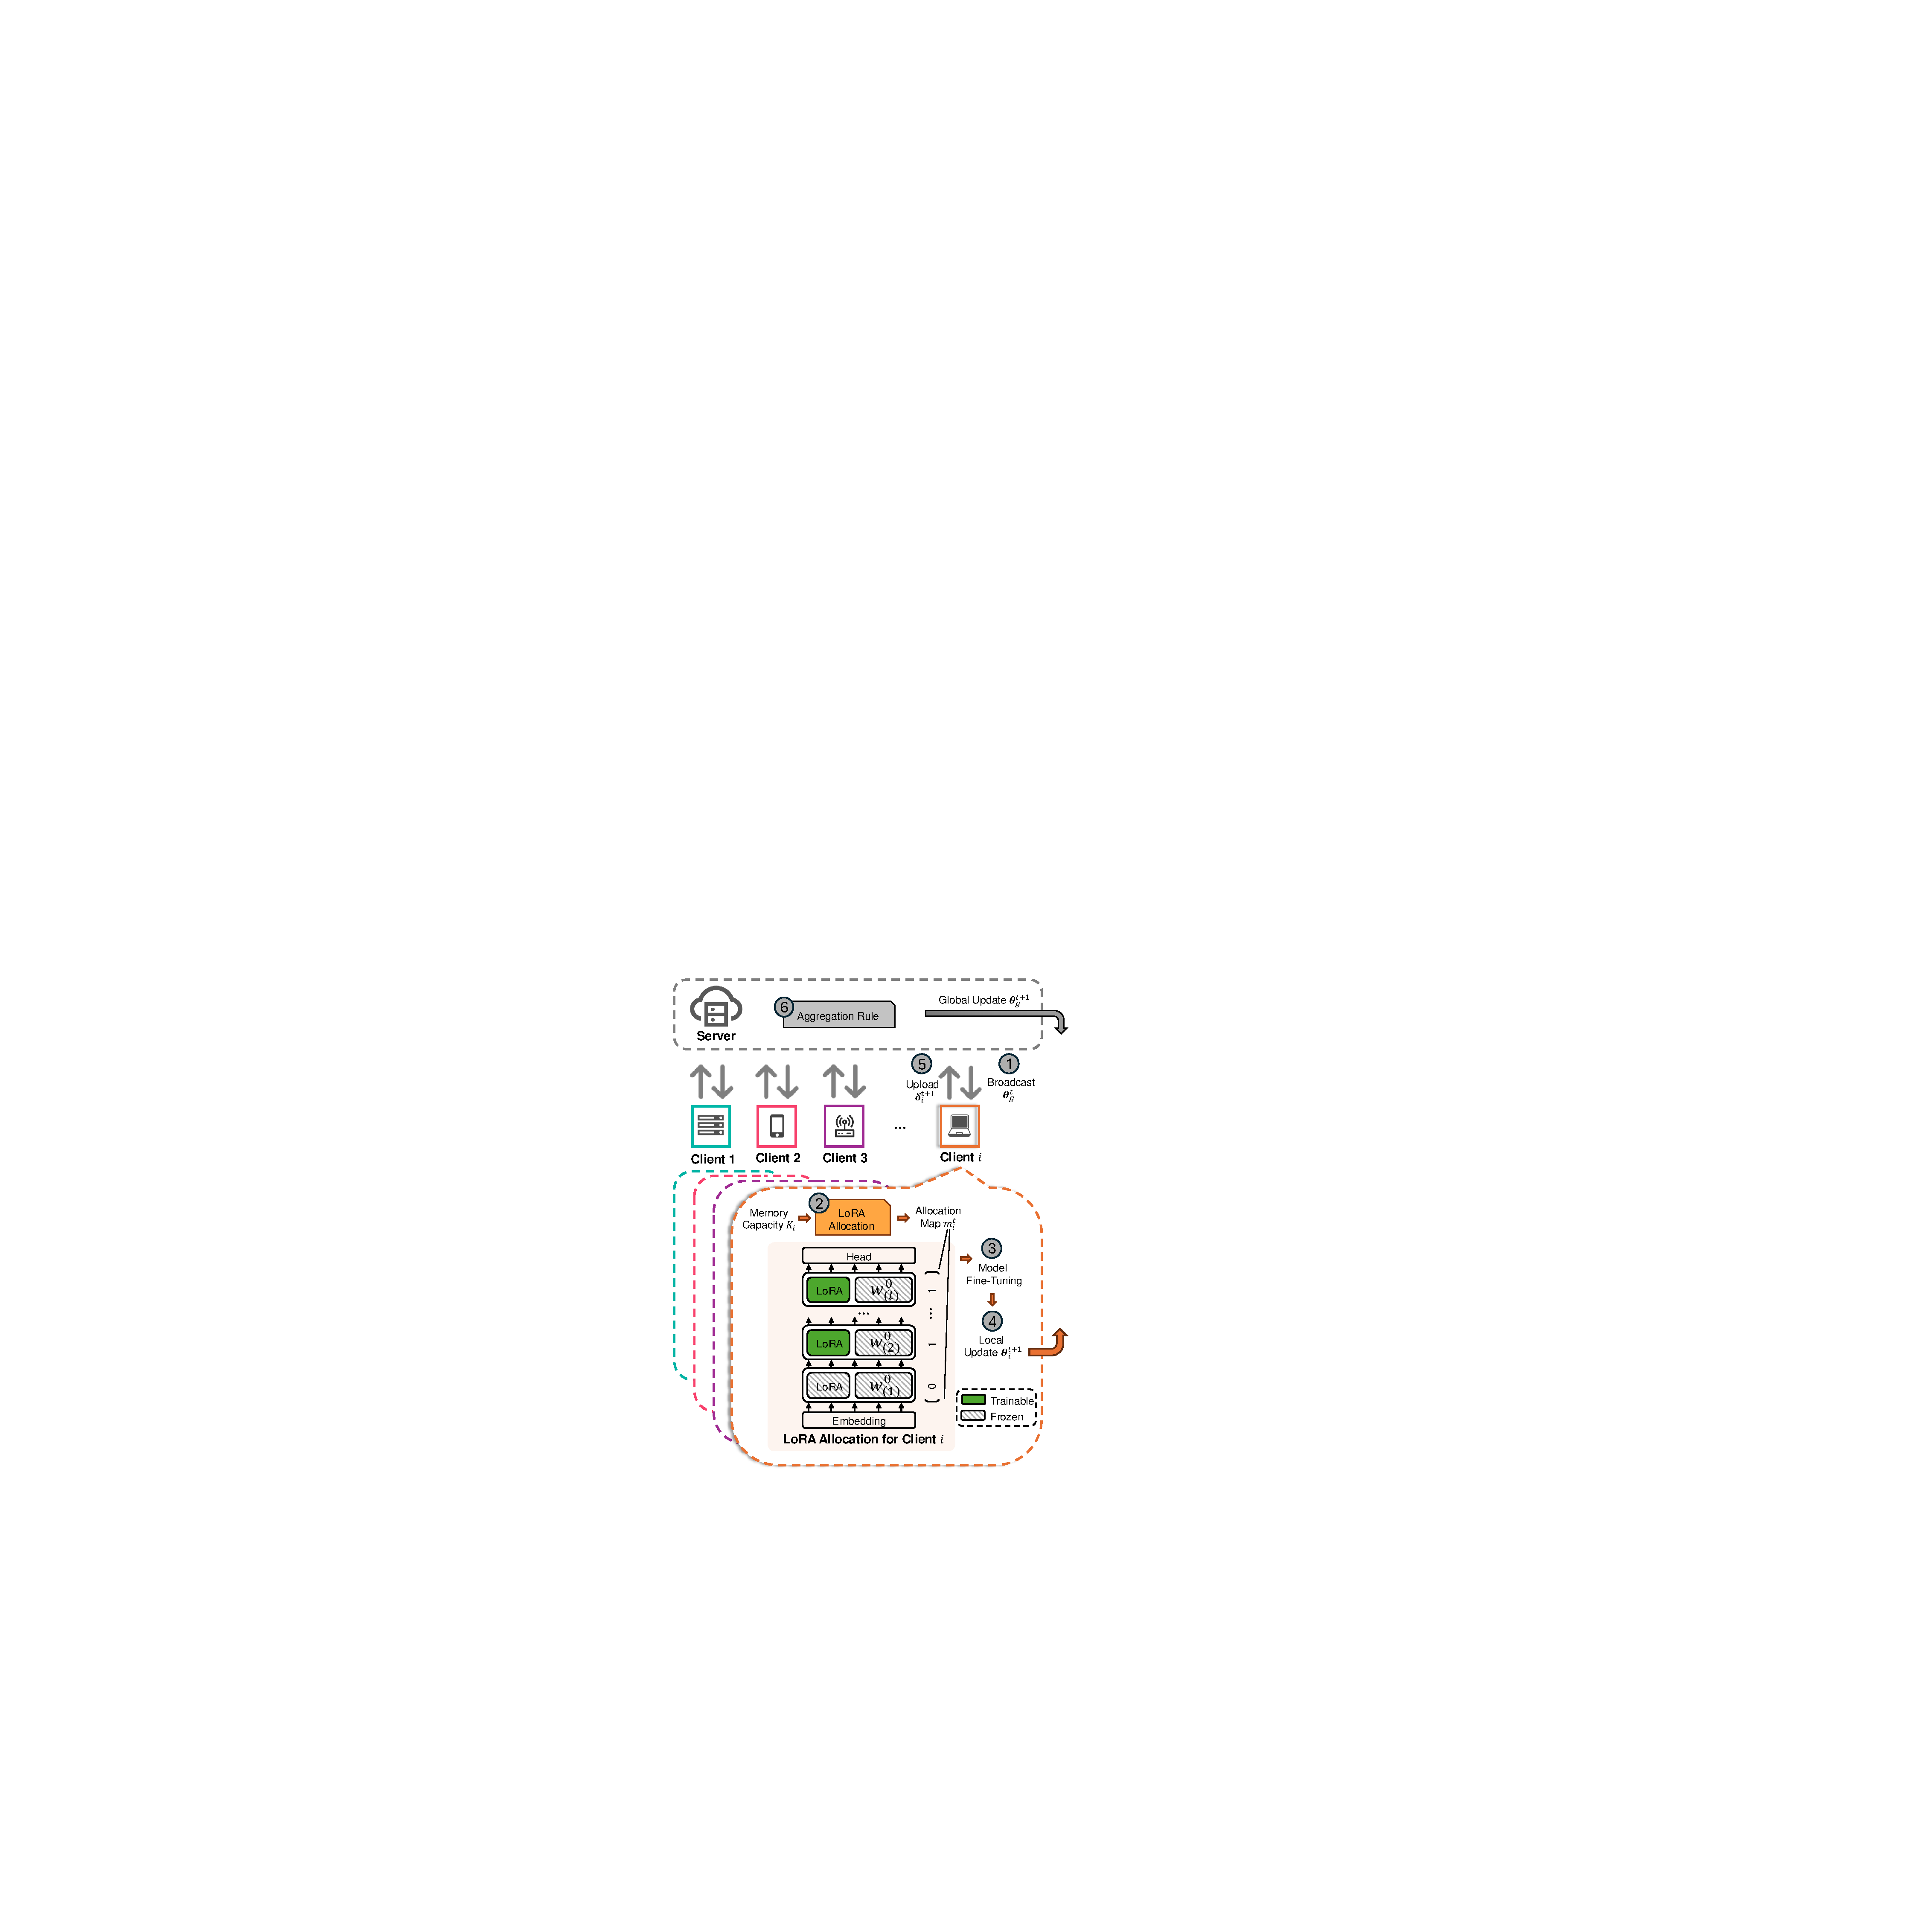
\includegraphics[width=0.40\textwidth]{fig/overallFramework.pdf}
% \vspace{-10pt}
\caption{The overall framework of Fed-pilot with optimal LoRA allocation over heterogeneous clients.}
\label{fig:framework}
\end{figure}

% % In this section, we introduce Fed-piLot, a framework designed to optimize LoRA allocation for efficient Federated Fine-Tuning. 
% In this section, we introduce Fed-piLot, an efficient federated fine-tuning framework tailored for clients with heterogeneous memory capabilities.
% % As shown in Figure~\ref{fig:framework}, each client operates under a memory consumption constraint, allowing them to fine-tune either a subset or all of the LoRA layers.
% % For instance, clients 1 through $i$ represent devices with varying GPU memory capacities, such as a server, a mobile phone, and a personal computer, respectively. 
% % Specifically, we assume that every client in the federated fine-tuning system operates under their memory constraints, which limits them to fine-tune only a subset of the LoRA layers.
% % On the client side, we implement LoRA allocation optimization to generate an allocation map for local fine-tuning. 
% % As shown in Fig.~\ref{fig:framework}, clients have devices with different memory capacities, and Fed-PiLot enables each client to fine-tune an optimal set of local LoRA layers under the coordination of the server. 
% % The core of Fed-piLot is to optimize the LoRA allocation locally for different clients.
% Specifically, we propose an IG-Score, which captures both local and global layer importance as the value function, while using memory consumption as the weight function to optimize global model performance.
% % On the server side, we propose STAgg with the LWSP strategy to mitigate noise resulting from varying model updates.
% In addition, we design a novel model aggregation rule, HAgg, which leverages historical information and accommodates heterogeneous local model updates arising from varying LoRA allocations.
% % In the following subsections, we define the optimization problem and describe the aggregation rule to achieve optimal global model performance.
% % In the following, we present the details of the LoRA allocation optimization and model aggregation.
% The following sections detail the optimization of LoRA allocation and the model aggregation process.

\subsection{Optimizing LoRA Allocation under Heterogeneous Memory Constraints}\label{sec:optlora}

% \subsubsection{LoRA Allocation}

% % Federated Fine-Tuning involves substantial memory consumption, which is not feasible for every client. 
% % As discussed earlier, activation memory constitutes the majority of overall memory consumption during the fine-tuning process. To enable efficient Federated Fine-Tuning, we propose LoRA allocation in our framework, allowing memory-limited clients to train only a subset of LoRA layers, constrained by their memory capacity.

% We define the memory capacity for each client $i$ as $\mathcal{K}_i$, where $\{\mathcal{K}_1, \mathcal{K}_2, \dots, \mathcal{K}_v\}$ may differ across clients. Based on our observation on the memory footprint of FM fine-tuning in Section~\ref{sec:memory_consumption}, reducing the number of trainable LoRA layers can significantly reduce the memory consumption. Specifically, assume each client $i$ has a LoRA allocation {map}
% % 
% % In round $t$, we define an allocation map 
% $m_i^t:=\{m_{i,(1)}^t, m_{i,(2)}^t, \cdots, m_{i,(l)}^t\}$
% % for each client $i$, 
% to represent the trainable status of each local LoRA layer in $\boldsymbol{\theta}_i^t$ in round $t$. Here, $m_{i,{(j)}}^t=1$ if the $j$-th LoRA layer is trainable, otherwise $m_{i,{(j)}}^t=0$ if it is frozen. {Based on this, after the local model initialization, the local trainable parameters are set as $\boldsymbol{\theta}_i^t := \{\Delta\boldsymbol{\mathcal{A}}_{(j)}\}_{j\in\mathcal{J}}$, where $\mathcal{J} = \{ j \mid m_{i,(j)}^t = 1,\forall j\}$.}
% Based on the allocation map,
% % we can compute the memory consumption for each client $i$. 
% the total memory consumption for client $i$ in round $t$ is formulated as, 
% \begin{equation}\label{eq:memory_model2}
% \begin{aligned}
% \mathcal{C}_{i}^t (m_i^t) = & \ b\zeta \varphi(\boldsymbol{\theta}_i^t)
%  + b\eta\sum_{j \in \mathcal{J}} \sigma_{d}(\boldsymbol{\mathcal{W}}_{i,(j)}^t) \\
%  & + {b\eta\sum_{j=j_{\min}
% }^{l}} \sigma_{s}(\boldsymbol{\mathcal{W}}_{i,(j)}) + \epsilon,
% \end{aligned}
% \end{equation}
% the first two terms indicate that the number of trainable LoRA layers influences the memory consumption of the optimizer state and dynamic activations. The third term shows that the memory consumption of static activations determined by the earliest trainable LoRA layer $j_{\min}=\min(\mathcal{J})$, since static activations from all layers after $j_{\min}$ must be stored for backpropagation~\cite{ardakani2024slimfit}. The memory consumption of model parameters 
% and the CUDA context are treated as a constant $\epsilon$. 
% % We define the memory capacity for each client $i$ as $\mathcal{K}_i$, with $\{\mathcal{K}_1, \mathcal{K}_2, \dots, \mathcal{K}_v\}$ potentially varying. 
% In practice, the memory consumption of a client cannot exceed its capacity, i.e., $\mathcal{C}_{i}^t \leq\mathcal{K}_i$ for $t\in[T]$. 

% Here, we illustrate two special cases to demonstrate how different LoRA allocations impact memory consumption. \textbf{Special Case 1: Memory Saver} designs the LoRA allocation map as $m_{\text{MS}}= \{0 \ \text{for} \ j \in [1, l-u], \ 1 \ \text{for} \ j \in [l-u+1, l]\}$, where the last $u$ LoRA layers are fine-tuned. \textbf{Special Case 2: Memory Hogger} designs the LoRA allocation map as $m_{\text{MH}}= \{1 \ \text{for} \ j \in [1, u], \ 0 \ \text{for} \ j \in [u+1, l]\}$, where the first $u$ LoRA layers are fine-tuned. Despite having the same number of trainable LoRA layers, the memory consumption difference between these two cases is $\mathcal{C}_{\text{MH}}-\mathcal{C}_{\text{MS}}={b\eta\sum_{j=1
% }^{l-u}} \sigma_{s}(\boldsymbol{\mathcal{W}}_{(j)})$, which can be substantial.


\subsubsection{Knapsack Optimization Problem}

% Since the information gain of each LoRA layer varies in its contribution to overall model performance~\cite{ardakani2024slimfit,zhang2022all}, it becomes crucial to consider this when assigning layers. To address this, we introduce a knapsack optimization problem that assigns LoRA layers in a way that satisfies the memory capacity while maximizing performance.

The knapsack optimization problem aims to maximize the total \textit{value} of selected \textit{items} while ensuring that their combined \textit{weight} does not exceed a predefined \textit{capacity}. In this context, \textit{value} corresponds to the utility or benefit of an {item}, while \textit{weight} represents its associated cost or resource consumption. The \textit{capacity} defines the maximum allowable total {weight} for the selected items.

In our setting, we employ knapsack optimization to maximize fine-tuning performance by optimizing the LoRA allocation map for each client under memory constraints. Specifically, for every client $i\in[v]$, we define the following constrained optimization problem: 
\begin{equation}\label{eq:optimization}
\max_{m_{i}} \sum_{j\in[l]}m_{i,(j)}{G}(\boldsymbol{\mathcal{\theta}}_{i, (j)}), \text{ subject to } \mathcal{C}(m_i) \leq\mathcal{K}_i.
\end{equation}
Here, ${G}(\cdot)$ is the value function, defined in \eqref{eq:valuefunction}, which quantifies the contribution of the LoRA module within a specific transformer block to the global model's performance.  $\mathcal{C}(\cdot)$ is the overall weight function, defined in \eqref{eq:memory_model2}, which measures the total memory consumption for a given allocation map. $\mathcal{K}_i$ denotes the memory capacity of client $i$. 

The problem is NP-hard in the discrete setting. The classical heuristic approach to solving it is the greedy algorithm, which iteratively selects items based on their value-to-weight ratio until reaching capacity. However, unlike standard knapsack optimization, where item weights are static, the weight of each LoRA module $\boldsymbol{\mathcal{\theta}}_{i, (j)}$ dynamically adapts based on the previously assigned LoRA modules. Specifically, at each step $h\in[0, l-1]$, the weight of an item $\boldsymbol{\mathcal{\theta}}_{i, (j)}$ is $\mathcal{C}_{i,(j)}^{h} = \mathcal{C}(m_i^h)$ if $h=0$, otherwise, 
\begin{multline}\label{eq:weightfunction}
\mathcal{C}_{i,(j)}^{h} = b\zeta\varphi(\boldsymbol{\mathcal{\theta}}_{i, (j)}) + b\eta\sigma_{(j)}^{d} \notag  \\
 + b\eta\sum_{j^{\prime}=\min(\mathcal{J}^{h-1} \cup \{ j \})}^{l} \sigma_{(j^\prime)}^{s} - b\eta\sum_{j^{\prime}=\min(\mathcal{J}^{h-1})}^{l} \sigma_{(j^\prime)}^{s},
\end{multline}
where $m_{i}^{h}$ represents the allocation map at step $h$ and $\mathcal{J}^{h-1} = \{ j \mid m_{i,(j)}^{h-1} = 1, \forall j \}$. Note that these item weights will be normalized using min-max scaling at every step.

% $\mathcal{G}(\boldsymbol{\mathcal{W}}_{i,(j)}^t)$ is the \textit{value} function, which is designed in Section~\ref{sec:IGScore}. 


% We use the contribution of a trainable LoRA layer to the global model's performance to represent its item value and the 
% The \textit{value} of an allocation represents its contribution to the global model's performance, while its \textit{weight} corresponds to the memory consumption incurred by training specific LoRA layers. 
% % The knapsack optimization problem emerges as we seek to maximize the overall global model performance by optimally assigning trainable LoRA layers, subject to memory capacity constraints. 
% \hl{Hence, the objective function can be formulated as,}
% \begin{equation}\label{eq:optimization}
% \begin{aligned}
% &\max_{\{m_{i}^t, \forall i, t\}} \sum_{t\in[T]}\sum_{i\in\mathbb{Q}^t}\sum_{j\in[1,l]}m_{i,(j)}^{t}\mathcal{G}(\boldsymbol{\mathcal{W}}_{i,(j)}^t), \\
% &\text{ subject to } \mathcal{C}_{i}^t(m_i^t) \leq\mathcal{K}_i, \forall i\in[v], t\in[T],
% \end{aligned}
% \end{equation}
% where $\mathcal{G}(\boldsymbol{\mathcal{W}}_{i,(j)}^t)$ is the \textit{value} function, which is designed in Section~\ref{sec:IGScore}. 
% %
% % To solve a knapsack problem, the classic method is to use a greedy algorithm to determine the optimal \textit{items} in an iterative manner. Specifically, at each step $h, 0 \leq h< l$, one LoRA layer will be chosen. 
% % %
% The \textit{weight} function is dynamic for each remaining LoRA layer $j$ for client $i$, based on the LoRA layer that has already been assigned which is denoted by $m_i^{h}$. For optimization step $h=0$, the \textit{weight} function follows the total memory consumption case in Equation~\eqref{eq:memory_model2} with $\sum_{i}^{l}m_i^{t,[h=0]}=1$. For $h>0$, 
% \begin{align}\label{eq:weightfunction}
% \mathcal{H}_{i}^{t,[h]}(j) 
% & = b\zeta\varphi(\boldsymbol{\mathcal{W}}_{i,(j)}^t) + b\eta\sigma_{d}(\boldsymbol{\mathcal{W}}_{i,(j)}^t) \notag \\
% & + b\eta\sum_{j^{\prime}=j_{\text{min}}^{[h]}}^{l} \sigma_{s}(\boldsymbol{\mathcal{W}}_{i,(j^{\prime})}) - b\eta\sum_{j^{\prime}=j_{\text{min}}^{[h-1]}}^{l} \sigma_{s}(\boldsymbol{\mathcal{W}}_{i,(j^{\prime})}) 
% \end{align}
% % % \begin{equation}\label{eq:weightfunction}
% % % \begin{aligned}
% % \begin{multiline}\label{eq:weightfunction}
% % \mathcal{H}_{i}^{h}(j) = 
% % b\zeta\varphi(\boldsymbol{\mathcal{W}}_{i,(j)}^t) + b\eta\sigma_{d}(\boldsymbol{\mathcal{W}}_{i,(j)}^t) + 
% % b\eta\sum_{j^{\prime}=j_{\text{min}}^{h}}^{l} \sigma_{s}(\boldsymbol{\mathcal{W}}_{i,(j^{\prime})})
% % \\ 
% % -b\eta\sum_{j^{\prime}=j_{\text{min}}^{h-1}}^{l} \sigma_{s}(\boldsymbol{\mathcal{W}}_{i,(j^{\prime})}) 
% %  % \end{aligned}
% %  \end{multiline}
% % \end{equation}
% $
% \text{with } \mathcal{J}^{[h-1]} = \{ j \mid m_{i,(j)}^{[h-1]} = 1 \}, \mathcal{J}^{[h]}=\mathcal{J}^{[h-1]} \cup \{ j \}, j_{\min}^{[h]} = \min(\mathcal{J}^{[h]}), \text{ and } j_{\min}^{[h-1]} = \min(\mathcal{J}^{[h-1]}).$
% Note that we use min-max scaling to normalize the \textit{weights}.

% To solve a knapsack problem, the classic method is to use a greedy algorithm to determine the optimal \textit{items} in an iterative manner. Specifically, at each step $h, 0 \leq h< l$, one LoRA layer will be chosen. 
% To solve a knapsack problem, a classic approach is to use a greedy algorithm to iteratively select the optimal \textit{items}. Specifically, at each step $h$, where $0 \leq h< l$, one LoRA layer is chosen.

\subsubsection{Information Gain Score based Value Function}\label{sec:IGScore}

Here, we define the value function used in our LoRA allocation optimization problem in \eqref{eq:optimization}, which quantifies the contribution of each LoRA module to fine-tuning performance.
% 
From an information-theoretic perspective, mutual information quantifies how much knowledge of one variable (e.g., a model parameter) reduces the uncertainty of another (e.g., task-specific loss) \cite{kullback1997information}. This suggests that a layer's importance in fine-tuning can be measured by how much information it contributes to minimizing the loss \cite{gabrie2018entropy}. However, directly computing mutual information in deep learning models is often intractable due to its high computational complexity.

To make this concept computationally feasible, we approximate a layer’s contribution using its gradient norm, which reflects how much a parameter influences loss reduction. A higher gradient norm indicates that a layer plays a more active role in optimization, capturing critical information necessary for improving model performance. Based on this intuition, we introduce the IG score $I_{(j)}$, a gradient-based metric that serves as a practical proxy for evaluating the information gain of the $j$-th LoRA module. 
\begin{equation}\label{eq:igscore}
I_{(j)}(\boldsymbol{\mathcal{\theta}}, D_{\text{IG}})=\sum^{ \lceil|D_{\text{IG}}|/|B^e_{\text{IG}}| \rceil}_{e=1}\left\|\nabla \ell(\boldsymbol{\mathcal{\theta}}; \boldsymbol{\Theta}^0, B_{\text{IG}}^e)_{(j)}\right\|_2^2,
\end{equation}
where $D_{\text{IG}}$ represents an IG dataset used to estimate the impact of each LoRA module, and $B_{\text{IG}}^{e}$ is a mini-batch sampled from $D_{\text{IG}}$ at the $e$-th forward-backward iteration. 

% % Directly defining a well-structured \textit{value} function in neural networks is challenging due to the complexity of capturing parameter contribution to model performance. 

% In information theory~\cite{kullback1997information}, 
% mutual information provides a potential approach to quantify how much knowledge of one variable (e.g., a model parameter) reduces uncertainty about another (e.g., task-specific loss), offering an information perspective on defining a \textit{value} function~\cite{gabrie2018entropy}.

% In practice, gradients indicate how much a parameter contributes to minimizing the loss $\mathcal{L}$, given the data and model. To better capture the contribution of each layer, we consider the gradient norm, which reflects the magnitude of change required for a specific layer to optimize the loss. This can be interpreted as the layer’s ability to ``gain'' critical information for improving the model’s performance. 
% Here, we introduce the IG-Score as follows,
% % , which measures the amount of information a model’s parameters contain about the data in a proxy dataset $D_{\text{IG}}$,
% \begin{equation}\label{eq:igscore}
% \Gamma_{(j)}=\sum^{ \lceil|D_{\text{IG}}|/|\vartheta^e_{\text{IG}}| \rceil}_{e=1}\|\nabla \ell(\boldsymbol{\mathcal{\theta}}; \boldsymbol{\Theta}^0, \vartheta_{\text{IG}}^e)_{(j)}\|_2^2,
% \end{equation}
% where $D_{\text{IG}}$ is a proxy dataset, $\vartheta_{\text{IG}}^{e}$ is a mini-batch sampled from $D_{\text{IG}}$, and $e$ represents the number of forward-backward iterations on $D_{\text{IG}}$.

% However, a key challenge arises: \textit{How can we obtain a generalized proxy dataset that is adaptable to all clients?}

However, calculating this IG score is challenging in federated settings. The server must obtain an IG dataset that aligns with the distribution of local datasets~\cite{zhu2021data}. However, if clients compute the IG score locally, the results may be sparse, when some LoRA modules are frozen and do not contribute to the gradient computation. Furthermore, when clients have Non-IID data distributions, a globally computed IG score may fail to reflect the client-specific importance of LoRA modules, leading to suboptimal LoRA allocation strategies. 

To address these challenges of sparsity and data heterogeneity, we design a three-step IG score aggregation process. Specifically, at round $t$, each client computes the IG score for its local trainable LoRA modules 
using a small subset $D_i^{\text{IG}}$ extracted from its local dataset, where the IG score for the $j$-th LoRA module is calculated by $I_{i,(j)}^t = I_{(j)} (\boldsymbol{\mathcal{\theta}}_i^{t}, D_i^{\text{IG}}) $ if $m_{i, (j)}^t = 1$.  
%and obtains $I_{i,(j)}^t=\{I_{i,(j)}^t; m_{i, (j)}^t = 1, \forall j\}$, where $I_{i,(j)}^t = I_{(j)} (\boldsymbol{\mathcal{\theta}}_i^{t}, D_i^{\text{IG}}) $. 
Let $\mathcal{V}_{(j)}^t = \{i; m_{i, (j)}^t = 1, i\in\mathcal{S}^t\}$ to represent the set of clients that train the $j$-th LoRA module at round \( t \) and $\mathcal{T}_{(j)}^t = \{t^\prime; \mathcal{V}_{(j)}^{t^\prime}\neq \emptyset, t^\prime \in (t-T_{\text{IG}}, t]\}$ to represent the set of past rounds in which at least one client trains the $j$-th LoRA module within the most recent \( T_{\text{IG}} \) rounds. Note that the temporal aggregation window$T_{\text{IG}}$ is selected to ensure that $\mathcal{T}_{(j)}^{t}\neq \emptyset$. Based on these, we define the value function of client $i$ as follows
\begin{align}\label{eq:valuefunction}
    {G}(\boldsymbol{\mathcal{\theta}}_{i, (j)}^t) = \frac{I_{i,(j)}^t + \frac{1}{|\mathcal{T}_{(j)}^t|}\sum_{t^\prime\in \mathcal{T}_{(j)}^t} \bar{I}_{(j)}^{t^\prime}}{{m_{i, (j)}^t + 1}} \nonumber\\ \text{ with } \bar{I}_{(j)}^{t^\prime} = \frac{1}{|\mathcal{V}_{(j)}^{t^\prime}|}\sum_{i\in \mathcal{V}_{(j)}^{t^\prime}} I_{i,(j)}^t.
\end{align}

To mitigate fluctuations and address sparsity in local scores, the value function first performs {cross-client aggregation} to compute an averaged IG score for each LoRA module. Then, it applies {temporal averaging} over the most recent \( T_{\text{IG}} \) rounds to further stabilize the score. Finally, to account for the unique data distribution of each client, the {temporally smoothed average score} is combined with the {client’s local score}, ensuring a balance between global knowledge and local adaptation in determining the final value of a LoRA module. %\hl{The detailed algorithm is given in Section~\ref{sec:appendix-algorithm} in Supplement.}




% Specifically, the IG-Score captures how sensitive the model’s predictions are to variations in its parameters, serving as an indicator of how much value each LoRA layer contributes to the model’s overall performance. We establish the IG-Score by characterizing the curvature of the likelihood function, which directly affects parameter updates during training through the gradient norm.

% Since federated fine-tuning is typically expose in settings where clients have Non-IID data distribution, maintaining a centralized proxy dataset~\cite{zhu2021data} on the server
% % Instead of collecting a proxy dataset on the server 
% and computing the score globally is inappropriate.
% % the \textit{Local-Global} IG-Score with Layer-Wise Sparse Pooling (LWSP) using local data.
% To address this, we propose computing the IG-Score locally on clients and aggregating scores on the server. However, given the clients' limited resources, effectively and efficiently crafting the IG-Score remains a non-trivial problem.

% \textbf{Client Side.}
% At round $t$, assume that client $i$ has a transformer model with LoRA layers $\boldsymbol{\Theta}_i^{t}=\{\boldsymbol{\mathcal{\theta}}_i^{t},\boldsymbol{\Theta}^0\}$ and a small IG dataset $D_{\text{IG}, i}^{t}$ randomly sampled from the local dataset $D_i$. 
% % For each mini-batch $\vartheta_{\text{IG},i}^{e}$, sampled from $D_{\text{IG},i}^t$ at the $e$-th iteration of the forward-backward process on the proxy dataset, the gradient norm is calculated as: $\gamma_{i,(j)}^{e,t}=\|\nabla \ell(\boldsymbol{\mathcal{\theta}}_i^t; \boldsymbol{\Theta}^0, \vartheta_{\text{IG}}^e)_{(j)}\|_2^2,$
% % For each mini-batch $\vartheta_{\text{IG},i}^{e}$ sampled from $D_{\text{IG},i}^t$, the client $i$ calculates the gradient norm as $\gamma_{i,(j)}^{e,t}=\|\nabla \ell(\boldsymbol{\mathcal{\theta}}_i^t; \boldsymbol{\Theta}^0, \vartheta_{\text{IG}}^e)_{(j)}\|_2^2$, where $e$ is the number of iteration of the forward-backward process on the IG dataset. {
% We obtain the IG-Score by 
% % \begin{equation}\label{eq:igscore}
% ${\hat{\Gamma}^t_{i,(j)}}=\sum^{ \lceil|D_{\text{IG},i}^t|/|\vartheta^e_{\text{IG},i}| \rceil}_{e=1}\gamma_{i,(j)}^{e,t}, \text{ if } j \in \mathcal{J}^{\prime}; \text{ otherwise, Null}$.
% % \end{equation}
% The set \(\mathcal{J}^{\prime}\) includes the indices \(j\) that are selected based on the client's memory capabilities (i.e., \(\mathcal{K}_i\)) to calculate the IG-Score for a layer.
% % , i.e., $\mathcal{J}^{\prime}={\{{j|\mathcal{C}_{i}^{t}}({\boldsymbol{\theta}_i^t=\boldsymbol{\mathcal{W}}_{i,(j)}^{t}})\leq\mathcal{K}_i}\}$ with Equation~\eqref{eq:memory_model2}
% % \footnote{Due to the linearity and independence of gradient computation in each layer, calculating the gradient for one LoRA layer at a time while freezing the others and then combining them yields the same result as computing the gradients for all LoRA layers simultaneously.}
% This IG-Score can be sparse. 

% However, the IG-Score ${\hat{\Gamma}^t_{i,(j)}}$ lacks a comprehensive view of a layer's information gain, as it is computed solely from local data. To address this, we incorporate a global IG-Score $\Gamma^t_{g,(j)}$, calculated on the server (discuss later), and define the \textit{value} function as follows,
% \begin{equation}\label{eq:lwsp}
% % {\Gamma^t_{i,(j)}}^{\prime\prime}
% \mathcal{G}(\boldsymbol{\mathcal{W}}_{i,(j)}^t)=
% % {\hat{\Gamma}^t_{i,(j)}}\oplus\Gamma^t_{g,(j)} =
% \frac{{\hat{\Gamma}^t_{i,(j)}} + \Gamma^t_{g,(j)}}{ \mathbf{1}_{{\hat{\Gamma}^t_{i,(j)}} \neq \text{Null}} + \mathbf{1}_{\Gamma^t_{g,(j)} \neq \text{Null}}}.
% \end{equation}
% This formulation computes a sparse average by summing the available IG-Scores per layer and dividing by the number of valid values, where $\mathbf{1}$ represents an indicator function. 
% % By applying min-max scaling $\hat{\cdot}$ to ${\Gamma^t_{i}}^{\prime\prime}:=\{{\Gamma^t_{i,(j)}}^{\prime\prime}\}_{j\in[l]}$, normalizing the values between 0 and 1, 
% The \textit{value} function is further normalized using min-max scaling.
% % Finally, we obtain the \textit{value} function using $\mathcal{G}(\boldsymbol{\mathcal{W}}_{i}^t)={{\Gamma^t_i}^{\prime\prime}}$. 

% To solve the reformulated problem in Section~\ref{subsec:lora-allocation} in a distributed manner, each selected client $i\in \mathbb{Q}^t$ employs a greedy algorithm to compute the optimal allocation map ${m_i^t}^{\star}$ that maximizes the local optimization objective: $\max_{m_i^t} \sum_{j\in[1,l]}m_{i,(j)}^{t}\mathcal{G}(\boldsymbol{\mathcal{W}}_{i,(j)}^t), \text{ s.t. } \mathcal{C}_{i}^t(m_i^t) \leq\mathcal{K}_i$.
% % , at round $t$. 
% % the Knapsack Optimization Problem using the greedy algorithm and obtain the optimal allocation map ${m_i^t}^{\star}$. 

% After local fine-tuning with ${m_i^t}^{\star}$, the client updates its local model $\boldsymbol{\theta}^{t+1}_i$ and recomputes the local IG-Score: $\Gamma^t_{i}:={\{\Gamma^t_{i,(j)}, j\in\{j|{m_i^t}^{\star}=1\}\}}$ using $D_{\text{IG},i}^t$ again.
% % only for the trained LoRA layers for calculating the \textit{Global} IG-Score, and 
% Finally, the client uploads both $\boldsymbol{\theta}^{t+1}_i$ and $\Gamma^t_{i}$ to the server.


% \textbf{Server Side.} To compute the global IG-Score, $\Gamma^{t+1}_g$, the server uses the operation in Equation~\eqref{eq:lwsp} to aggregate Local IG-Scores over the most recent \(N_{\text{IG}}\) rounds. 
% % for each client. Then it applies LWSP again to combine the aggregated \textit{Local} IG-Scores of all clients to be the final \textit{Global} IG-Score. 
% % , which is formulated as: $\Gamma^{t+1}_g = 
% % \oplus_{t' \in [t-N_{\text{IG}}+1, t]} \oplus_{i \in \mathbb{Q}^{t'}} \Gamma^{t'}_i$. 
% % This method aggregates the IG-Scores not only across clients within each round but also over the past \(N_{\text{IG}}\) rounds, improving the stability and consistency of global IG-Score over time. 

% To summarize, the complete process is detailed in the algorithm provided in Section~\ref{sec:appendix-algorithm} of the Supplement.

% \begin{figure}[t]
% \centering
% \includegraphics[width=0.48\textwidth]{fig/agg.pdf}
% % \vspace{-10pt}
% \caption{An example of the proposed HAgg rule.}
% \label{fig:agg}
% % \vspace{-12pt} 
% \end{figure}

\subsection{Aggregation with Update Compensation}\label{subsec:HAgg}

With optimized LoRA allocation, clients with varying memory capacities train different sets of LoRA modules, leading to diverse model updates. From a global perspective, this divergence causes variations in both the frequency and the {scale} of the parameter changes across LoRA modules. Specifically, some modules receive updates from a larger number of clients, while others receive updates from fewer clients. As a result, due to the Non-IID nature of client data, different layers may learn from distinct data distribution. In this case, simply averaging model updates can hinder convergence. 

To address this issue, we design a compensated aggregation rule ({ComAgg}), which dynamically compensates the layers that are less updated at the current round. Specifically, upon received the local model updates $\{\boldsymbol{\delta}_i^{t+1}\}_{i\in \mathcal{S}^t}$ from the selected clients at round $t$, the server aggregates them layer-wise as follows: for each $j\in[l]$,
\begin{align}\label{eq:agg_temporal}
    {\boldsymbol{\delta}}_{(j)}^{t+1} =  \frac{\beta_{(j)}^t}{\alpha_{(j)}^t+\beta_{(j)}^t}\boldsymbol{\delta}_{(j)}^{t} + \frac{\alpha_{(j)}^t}{\alpha_{(j)}^t+\beta_{(j)}^t} \bar{\boldsymbol{\delta}}_{(j)}^{t+1} \nonumber\\
    \text{ with } \bar{\boldsymbol{\delta}}_{(j)}^{t+1} = \frac{1}{|\mathcal{S}_{(j)}^t|} \sum_{i \in \mathcal{S}_{(j)}^t} {\boldsymbol{\delta}}_{i, (j)}^{t+1},
\end{align}
where $\mathcal{S}_{(j)}^t = \{i; m_{i, (j)}^t=1, i\in \mathcal{S}^t\}$ represents the set of clients that train the $j$-th LoRA module at round $t$. The coefficient $\alpha_{(j)}^t=|\mathcal{S}_{(j)}^t|$ represents the number of clients training the $j$-th LoRA module at round $t$, and $\beta_{(j)}^t=\frac{1}{ T_{\text{Agg}}} \sum_{t^\prime = t - T_{\text{Agg}} + 1}^{t} \alpha_{(j)}^{t^\prime}$ captures the average number of clients contributing to the $j$-th LoRA module over the past $T_{\text{Agg}}$ rounds. By compensating under-updated LoRA modules using historical global updates, ComAgg mitigates inconsistencies in data distribution across modules, ensuring more stable convergence.



% This imbalance results in certain layers receiving more contributions while others are influenced by only a few clients, introducing potential domain biases and hindering global model convergence.

% % introduces significantly higher aggregation noise compared to homogeneous cases. 
% In this section, we propose a novel aggregation rule called HAgg. By incorporating historical model updates with dynamic weights, it enables a smooth and robust accumulation of local updates.
% % Additionally, the DWA strategy is employed to reduce the divergence of heterogeneous model updates.
% At round $t$, each selected client $i$ uploads the local update $\boldsymbol{\delta}_i^{t+1} := \{\boldsymbol{\delta}_{i,(j)}^{t+1}\}_{j=1}^{l}$
% % and the allocation map $m_i^t$ 
% to the server. 
% %
% % We first define the spatial aggregation rule as follows,
% % \begin{equation}\label{eq:agg_spatial}
% %     \boldsymbol{\delta}_{g,S}^{t+1} = \left\{\frac{1}{\sum_{i\in\mathbb{Q}^t} m_{i,(j)}} \sum_{i\in\mathbb{Q}^t}m_{i,(j)} \boldsymbol{\delta}_{i,(j)}^{t+1} \right\}_{j=1}^{l},
% % \end{equation}
% % which averages the local model updates.
% % Next, 
% %
% We define HAgg as follows,
% % with the DWA strategy 
% \begin{equation}\label{eq:agg_temporal}
%     \tilde{\boldsymbol{\delta}}_{i}^{t+1} = \left\{\frac{\alpha_{(j)}^t}{\alpha_{(j)}^t+\beta_{(j)}^t}\boldsymbol{\delta}_{i,(j)}^{t+1} + \frac{\beta_{(j)}^t}{\alpha_{(j)}^t+\beta_{(j)}^t}\boldsymbol{\delta}_{g,(j)}^{t}\right\}_{j=1}^{l},
% \end{equation}
% where $\alpha^t:=\{\alpha_{(j)}^t\}_{j=1}^{l} \text{ with }\alpha_{(j)}^t=\sum_{i\in\mathbb{Q}^t}m_{i,(j)}^t$ represents the number of clients that contribute to each LoRA layer in the current round, and $\beta^t:=\{\beta_{(j)}^t\}_{j=1}^{l} \text{ with } \beta_{(j)}^t=\frac{1}{N_{\text{H}}} \sum_{t' = t - N_{\text{H}} + 1}^{t} \alpha_{(j)}^{t'}$ denotes the historical average number of clients that contributed to the $j$-th LoRA layer over the past $N_{\text{H}}$ rounds. After obtaining the smoothed local update $\tilde{\boldsymbol{\delta}}_i^{t+1}$, it follows the aggregation rule in Equation~\eqref{eq:newagg} to update the global model.

% In Figure~\ref{fig:agg} we illustrate an example of our proposed HAgg rule using a three-layer transformer model. In each round $t$, all clients share the same $\alpha^t$ and $\beta^t$. When only one client contributes to the first layer ($\alpha^t_1=1$) in a given round, the final model update is not dominated by this single client but is instead smoothed using historical global model updates.




%
% $\boldsymbol{\mathcal{\theta}}_g^{t+1} := \boldsymbol{\mathcal{\theta}}_g^t + ({1}/{q})\sum_{i\in \mathbb{Q}^t}\boldsymbol{\delta}_i^{t+1},$ which results in the global model $\boldsymbol{\Theta}_g^{t+1}=\{\boldsymbol{\mathcal{\theta}}_g^{t+1};\boldsymbol{\Theta}^0\}$ 

% Table for CIFAR-100
\begin{table}[t]
  \centering
  \caption{Main results on CIFAR-100 dataset with ViT-base model in both IID and Non-IID settings.}
  \scalebox{0.88}{
    \begin{tabular}{c|cccc}
    \toprule[1pt]
    % \textbf{Dataset/Model/Metric/Capacity} 
    \multirow{2}{*}{\textbf{Methods}} & \multicolumn{4}{c}{\textbf{Model Performance (Accuracy)}} 
    %\multicolumn{7}{c}{\textbf{Natural-Instruction / Llama / Rouge-L / Memory Capacity Levels: V100 32 GB, A100 40 GB, A6000 48 GB, H100 80 GB}} 
    \\
    \cline{2-5}
    % \textbf{Methods} 
    & \textbf{IID} & \textbf{Non-IID (20)} & \textbf{Non-IID (10)} & \textbf{Avg} \\
    \midrule
    Baseline-EL & 40.15 & 27.82 & 7.04  & 25.00 \\
    Baseline-MH & 53.36 & 29.77 & 7.92  & 30.35 \\
    Baseline-MS & 76.38 & 68.34 & 57.63 & 67.45 \\ \midrule
    FLoRA &1.61 &0.90 &0.78 &1.09 \\
    FlexLoRA &1.84 &1.92 &1.86 &1.87 \\
    HETLoRA &6.91 &8.23 &1.59 &5.57 \\
    FedRA & 72.60 & 62.95 & 47.98 & 61.17 \\
    \midrule
    \textbf{Ours} & \cellcolor[rgb]{ .91,  .91,  .91}80.09 & \cellcolor[rgb]{ .91,  .91,  .91}73.35 & \cellcolor[rgb]{ .91,  .91,  .91}63.93 & \cellcolor[rgb]{ .91,  .91,  .91}72.45 \\
    \bottomrule[1pt]
    \end{tabular}%
    }
  \label{tab:cifar100-results}%
\end{table}

% Table for LEDGAR
\begin{table}[t]
  \centering
  \caption{Main results on LEDGAR dataset with BERT-base model in both IID and Non-IID settings.}
  \scalebox{0.88}{
    \begin{tabular}{c|cccc}
    \toprule[1pt]
    % \textbf{Dataset/Model/Metric/Capacity} 
    \multirow{2}{*}{\textbf{Methods}} & \multicolumn{4}{c}{\textbf{Model Performance (MacroF1)}} 
    %\multicolumn{7}{c}{\textbf{Natural-Instruction / Llama / Rouge-L / Memory Capacity Levels: V100 32 GB, A100 40 GB, A6000 48 GB, H100 80 GB}} 
    \\
    \cline{2-5}
    % \textbf{Methods} 
    & \textbf{IID} & \textbf{Non-IID (20)} & \textbf{Non-IID (10)} & \textbf{Avg} \\
    \midrule
    Baseline-EL & 60.76 & 43.94 & 0.12  & 34.94 \\
    Baseline-MH & 61.58 & 6.59  & 0.22  & 22.79 \\
    Baseline-MS & 62.95 & 56.22 & 46.93 & 55.36 \\ \midrule
    FLoRA &0.10 &0.07 &0.01 &0.06 \\
    FlexLoRA &0.10 &0.24 &0.32 &0.22 \\
    HETLoRA &0.51 &0.32 &0.10 &0.31 \\ 
    FedRA & \cellcolor[rgb]{ .91,  .91,  .91}63.20 & 54.96 & 47.24 & 55.13 \\
    \midrule
    \textbf{Ours} & 63.17 & \cellcolor[rgb]{ .91,  .91,  .91}56.31 & \cellcolor[rgb]{ .91,  .91,  .91}48.87 & \cellcolor[rgb]{ .91,  .91,  .91}56.11 \\
    \bottomrule[1pt]
    \end{tabular}%
    }
  \label{tab:ledgar-results}%
\end{table}



% \begin{figure*}[t]
% \centering
% \includegraphics[width=0.93 \textwidth]{fig/ledgar-macrof1-loss.pdf}
% % \vspace{-10pt}
% \caption{LEDGAR.}
% \label{fig:ledgar-macrof1-loss}
% % \vspace{-12pt} 
% \end{figure*}

\section{Evaluation}\label{evaluation}
\subsection{Experimental Settings}
\subsubsection{Memory Capacity Heterogeneity}
% We introduce resource heterogeneity among FL clients by varying their memory capacities. 
%
% To generalize, we categorize clients into four groups representing distinct memory capacity levels: very low, low, medium, and high.
%
% Practically, we determine these four memory capacity levels by averaging the memory consumption in both Memory Saver and Memory Hogger modes when training with ``1/4'', ``1/2'', ``3/4'', or ``full'' numbers of LoRA layers (see Section~\ref{sec:appendix-capacity-calculation} in Supplement).
% Practically, we 
We define four memory capacity levels (Level 1-4) based on real-world NVIDIA GPUs. For FMs with millions of parameters, we set the client memory capacities to 24 GB, 32 GB, 40 GB, and 48 GB for Level 1 through 4, respectively. For FMs with billions of parameters, the corresponding memory capacities are to 32 GB, 40 GB, 48 GB, and 80 GB. See {{Supplement Section~\ref{subsec:appendix-capacity-settings}}} for detailed capacity settings on different models. We assume that clients are distributed across these levels in a 4:3:2:1 ratio, from the lowest to the highest memory capacity, reflecting the higher prevalence of low-memory clients in real-world scenarios.

% We then assign clients to these levels in a 4:3:2:1 ratio, reflecting the prevalence of low-memory clients in real-world scenarios. 
% This approach effectively simulates the resource heterogeneity observed in practical applications.

\subsubsection{Data Heterogeneity}

We evaluate our approach on five distinct datasets while simulating varying levels of Non-IID settings, including category heterogeneity, task heterogeneity, and domain heterogeneity.
% Additionally, we introduce data volume heterogeneity (i.e., the number of data points on each client's device) into all experiments using a Dirichlet distribution factor, $Dir$. 



\textbf{Category Heterogeneity.} We use CIFAR-100 dataset~\cite{krizhevsky2009learning} and LEDGAR dataset from LexGLUE~\cite{chalkidis-etal-2021-lexglue} to simulate the category heterogeneity settings by skewing the label distribution across clients. For the pre-trained model, we use ViT-base~\cite{dosovitskiy2020image} for visual tasks and BERT-base~\cite{devlin2019bert} for language tasks. 
% To evaluate the impact of category heterogeneity by skewing the labels, we conduct experiments on CIFAR-100 dataset~\cite{krizhevsky2009learning} and LEDGAR dataset from LexGLUE~\cite{chalkidis-etal-2021-lexglue}. 
% Each of the dataset has 100 categories with visual or text objects, respectively. 
% We skew the datasets by assigning 20, and 10 categories of data samples for each client to fully evaluate the real-world category heterogeneity effects. 
% We use ViT-base~\cite{dosovitskiy2020image} for visual tasks and BERT-base~\cite{devlin2019bert} for language tasks.
% Results are reported in Accuracy for visual tasks and in Macro F1 for language tasks.

\textbf{Task Heterogeneity.} We use Natural Instruction (NI) dataset~\cite{wang2022super} and Dolly-15K~\cite{conover2023free} dataset that contain diverse natural language tasks to evaluate our approach under task heterogeneity. 
% The NI dataset consists of 1,616 diverse natural language tasks with instructions,  and answers. 
% We simulate three levels of task heterogeneity from IID to extreme Non-IID, by varying the number of client's data tasks to full, 20, and 15 for NI and full, 3, and 1 for Dolly-15K. 
% The Dolly-15K dataset is a instructiona-following record dataset that generated by human and Wikipedia. 
% The Dolly-15K dataset includes 8 tasks with instructions, contexts, and responses.
% Due to the limited computing resources, w
We use a Llama-like model Data-Juicer-1B~\cite{chen2024data} and the OPT-1.3B~\cite{zhang2022opt} as the pre-trained models for these two datasets, respectively. 
% All reported results are based on the metric called Rough-L.


\textbf{Domain Heterogeneity.} 
% Domain discrepancy is commonly seen in the dataset from distributed clients, we implement experiments on a 
We use a customized DomainNet dataset~\cite{peng2019moment} (referred to as DomainNet-121), which contains six visual domains, to simulate the domain heterogeneity by assigning data from only one domain to each client. For this dataset, we use ViT-base~\cite{dosovitskiy2020image} as the pre-trained model. 

We provide the details of data settings in {{Supplement Section~\ref{sec:appendix-dataset}}}.
% including clipart, real-world images, sketch, infograph, painting, and quickdraw. F
% and for each client we only assign one domain of data.
% with a number of categories.
% varying from full, 50, and 25. All results are reported with Accuracy.


% We conduct experiments on both visual and language tasks. For visual tasks, we use the CIFAR-100 dataset~\cite{krizhevsky2009learning} and a customized DomainNet dataset~\cite{peng2019moment} (referred to as DomainNet-121). 
% For the language task, we use the LEDGAR dataset from LexGLUE~\cite{chalkidis-etal-2021-lexglue}. We simulate three levels of data heterogeneity (from IID to extreme Non-IID) for federated fine-tuning by varying clients' data quantities, labels, or domains. 
% For example, at the ``20/1.0'' level, clients have 20 categories with data skewed by a Dirichlet distribution ($\alpha=1.0$); at the ``50/1'' level, clients have 50 categories and 1 domain per category. 
% We use
% focus on models with up to 1 million parameters
% ~\cite{cho2023heterogeneous}, using 
% ViT-base~\cite{dosovitskiy2020image} for visual tasks and BERT-base~\cite{devlin2019bert} for language tasks. 
% LoRA layers are applied to the ``query'' and ``value'' modules in each transformer layer, with the rank, scaling parameter, and dropout probability set as 16, 16, and 0.1, respectively. 
% For evaluation metrics, we use top-1 accuracy for CIFAR-100 and DomainNet-121, and Macro F1 score for LEDGAR~\cite{chalkidis-etal-2021-lexglue}.
% In the FL experiments, we use $v=100$ clients, with the local epoch of 1 and training rounds $T=350$. In each round, the server randomly selects $q=10$ clients for local fine-tuning using the AdamW optimizer and a batch size of 8. 
% We use the average memory consumption of both Memory Saver and Memory Hogger when training 3, 6, 9, or 12 LoRA layers to represent four distinct levels of memory capabilities: very low, low, median, and high. We set the numbers of clients for very low, low, median, and high levels as 40, 30, 20, and 10, considering the a large proportion of low-memory clients in practice. 
% In a practical scenario with a large proportion of low-memory clients, we set the number of clients to 40, 30, 20, and 10, with memory capability defined based on training 3, 6, 9, or 12 LoRA layers, corresponding to various memory capacities. For example, a client with memory capability for 3 LoRA layers, it is averaged between training the first 3 layers and the last 3 layers of a 12-layer transformer model.
% In all experiments, both $N_{\text{IG}}$ and $N_{\text{DWA}}$ are set to 10, and $|D_{\text{IG}}|$ is 50.



\subsubsection{Baselines}
To evaluate the effectiveness of Fed-pilot, we implement seven baselines:

\textit{Baseline-Exclusive Learning (EL)} excludes clients that cannot train all LoRA modules. 
%
\textit{Baseline-Memory Saver (MS)} allocates the last $u$ LoRA modules according to the capacity, prioritizing the training of more modules.
% , $m_{\text{MS}} = \{0 \ \text{for} \ j \in [1, l - u_{\text{MS}}], \ 1 \ \text{for} \ j \in [l - u_{\text{MS}} + 1, l]\}$.
%
\textit{Baseline-Memory Hogger (MH)} allocates the first $u$ LoRA modules according to the capacity,
% $m_{\text{MH}} = \{1 \ \text{for} \ j \in [1, u_{\text{MH}}], \ 0 \ \text{for} \ j \in [u_{\text{MH}} + 1, l]\}$, 
emphasizing the utilization of shallow-layer features.
% The chose of $u_{\text{MS}}$ and $u_{\text{MH}}$ is subject to clients' memory capacity.
%
{HETLoRA}~\cite{cho2024heterogeneous} is a rank-based method designed to accommodate heterogeneous clients with varying LoRA ranks.
%
{FLoRA}~\cite{wangflora} assigns lower ranks to resource-constraint clients and shares stacked LoRA modules for updates.
%
{FlexLoRA}~\cite{bai2024federated} improves aggregation in rank-based methods using SVD.
%
{FedRA}~\cite{su2023fedra} 
% is a federated LoRA-based fine-tuning framework that 
randomly allocates a subset of LoRA modules for clients with limited memory capacities to train at each round. 
%We adapt these baselines to our scenario, ensuring that layers are dropped as needed to meet each client's memory constraints.

\subsubsection{Implementation Details}
% 47 * 3 * 2 * 8 + 16 * 3 * 2 * 8
We use PyTorch to implement our framework. All experiments are carried out on a server with 8 $\times$ NVIDIA RTX A6000 GPUs. The total GPU hours for running all the experiments are over 3,000 GPU hours. For the configuration of models,  hyper-parameters, and FL settings, 
please refer to {{Supplement Section~\ref{sec:appendix-settings}}} for more details.

% \begin{figure}[t]
% \centering
% \includegraphics[width=0.50\textwidth]{fig/domainnet121-accuracy.pdf}
% % \vspace{-10pt}
% \caption{Testing accuracy on DomainNet-121 under different Non-IID settings.
% % (Memory capacity levels are identical to CIFAR-100 and LEDGAR).
% }
% \label{fig:domainnet121-accuracy}
% % \vspace{-12pt} 
% \end{figure}

\begin{figure}[t]
\centering
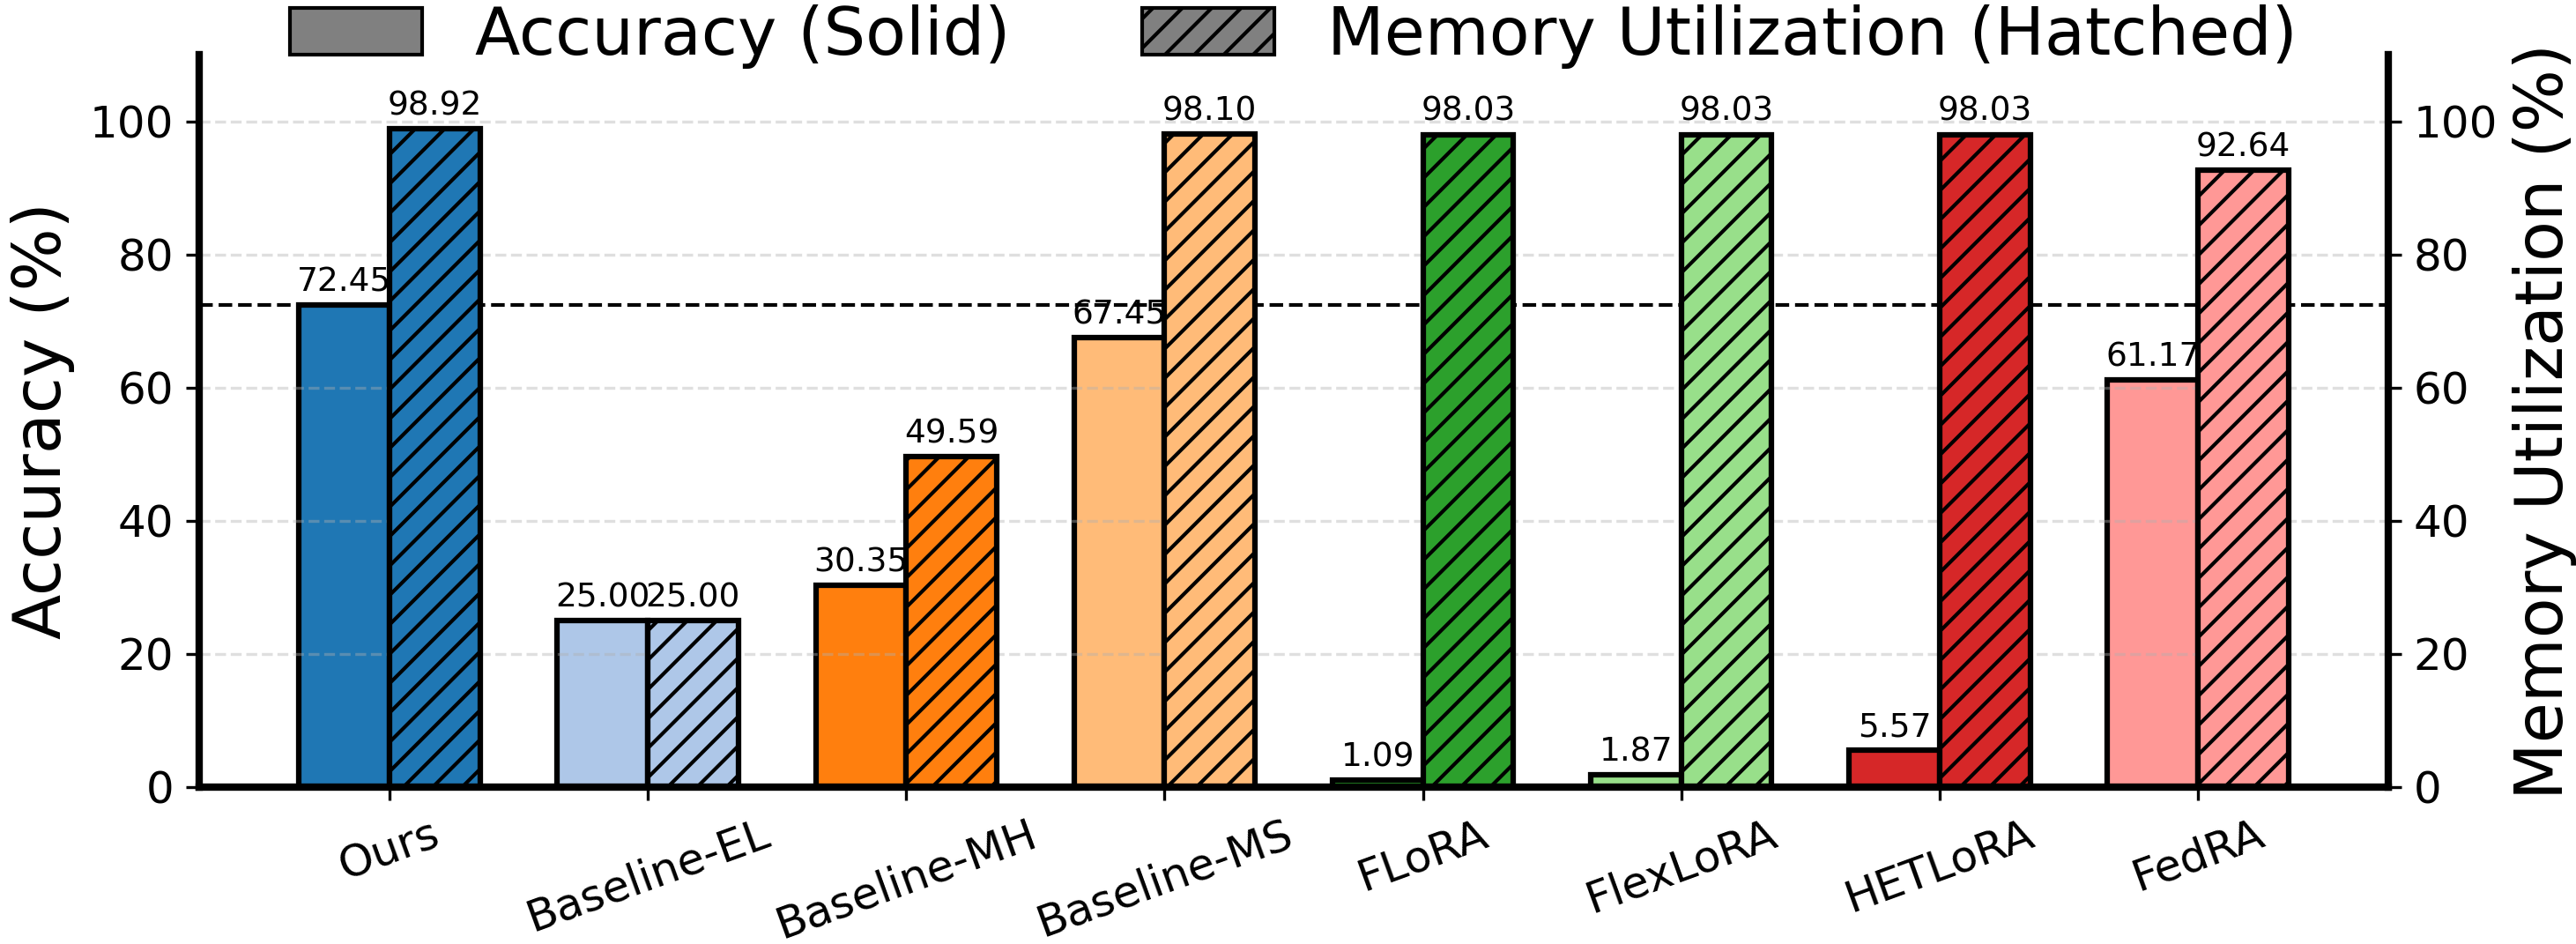
\includegraphics[width=0.48\textwidth]{fig/accuracy_vs_memory_dual_axis.png}
% \vspace{-10pt}
\caption{The average accuracy vs. average memory utilization across methods on CIFAR-100 dataset.}
\label{fig:memory_utilization}
\end{figure}


\begin{figure*}[t]
\centering
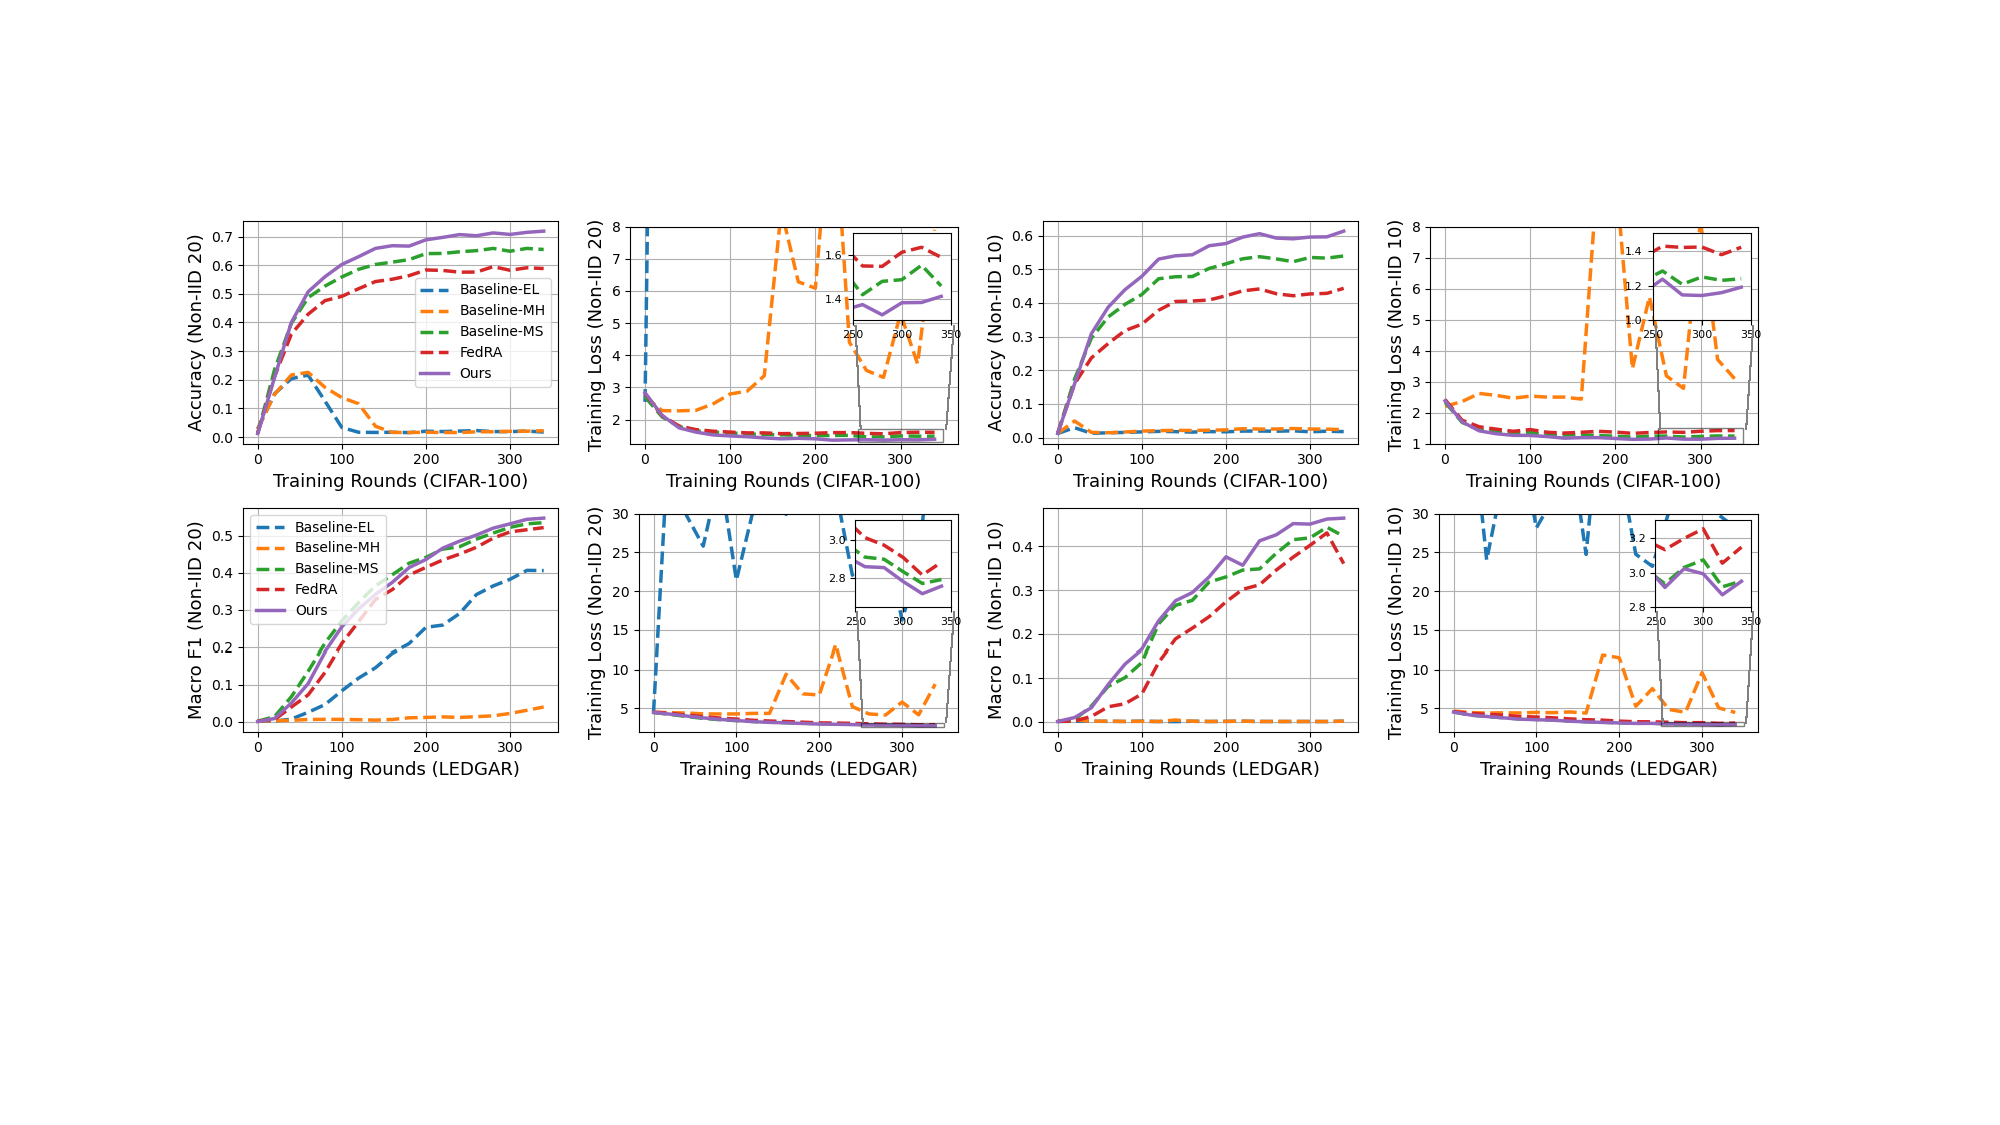
\includegraphics[width=0.95 \textwidth]{fig/cifar100-ledgar-metric-loss.pdf}
% \vspace{-5pt}
\caption{Convergence performance on CIFAR-100 and LEDGAR datasets. Rank-based methods are excluded from the results as they diverge.}
\label{fig:cifar100-ledgar-metric-loss}
% \vspace{-12pt} 
\end{figure*}

\subsection{Experimental Results}

% % Table generated by Excel2LaTeX from sheet 'Sheet1'
% \begin{table*}[htbp] % htbp
%   \centering
%   \scalebox{0.92}{
%     \begin{tabular}{c|cccc|cccc|cccc}
%     \toprule[1pt]
%     \textbf{Dataset/Model/Metric} & \multicolumn{4}{c|}{\textbf{CIFAR-100/ViT-base/Acc}} & \multicolumn{4}{c|}{\textbf{DomainNet-121/ViT-base/Acc}} & \multicolumn{4}{c}{\textbf{LEDGAR/BERT-base/MacroF1}} \\
%     \midrule
%     % \textbf{Metric} & \multicolumn{4}{c|}{\textbf{Accuracy}} & \multicolumn{4}{c|}{\textbf{Accuracy}} & \multicolumn{4}{c}{\textbf{Macro F1}} \\
%     % \midrule
%     \textbf{Methods/DH} & \textbf{IID} & \textbf{20/1.0} & \textbf{10/1.0} & \textbf{Avg} & \textbf{IID} & \textbf{50/1} & \textbf{25/1} & \textbf{Avg} & \textbf{IID} & \textbf{20/1.0} & \textbf{10/1.0} & \textbf{Avg} \\
%     \midrule
%     Exclusive & 40.15 & 27.82 & 7.04  & 25.00 & 50.33 & 38.34 & 21.15 & 36.60 & 60.76 & 43.94 & 0.12  & 34.94 \\
%     Baseline-MH & 53.36 & 29.77 & 7.92  & 30.35 & 50.19 & 38.20 & 19.61 & 36.00 & 61.58 & 6.59  & 0.22  & 22.79 \\
%     Baseline-RD & 72.60 & 62.95 & 47.98 & 61.17 & 57.38 & 53.05 & 38.07 & 49.50 & \cellcolor[rgb]{ .91,  .91,  .91}63.20 & 54.96 & 47.24 & 55.13 \\
%     Baseline-MS & 76.38 & 68.34 & 57.63 & 67.45 & 58.92 & 53.60 & 40.82 & 51.11 & 62.95 & 56.22 & 46.93 & 55.36 \\
%     \midrule
%     \textbf{Ours} & \cellcolor[rgb]{ .91,  .91,  .91}80.09 & \cellcolor[rgb]{ .91,  .91,  .91}73.35 & \cellcolor[rgb]{ .91,  .91,  .91}63.93 & \cellcolor[rgb]{ .91,  .91,  .91}72.45 & \cellcolor[rgb]{ .91,  .91,  .91}59.36 & \cellcolor[rgb]{ .91,  .91,  .91}54.40 & \cellcolor[rgb]{ .91,  .91,  .91}42.20 & \cellcolor[rgb]{ .91,  .91,  .91}51.98 & 63.17 & \cellcolor[rgb]{ .91,  .91,  .91}56.31 & \cellcolor[rgb]{ .91,  .91,  .91}48.87 & \cellcolor[rgb]{ .91,  .91,  .91}56.11 \\
%     \bottomrule[1pt]
%     \end{tabular}%
%     }
%   \caption{Main Results of Fed-piLot Compared with Baselines on CIFAR-100, DomainNet-121, and LEDGAR datasets.}
%     % \vspace{-11pt}
%   \label{tab:main-alldataset}%
% \end{table*}%

% We assess the effectiveness of our Fed-piLot framework across three datasets,
% each evaluated under three different levels of data heterogeneity, 
% and compare the results with baselines. 
% The main experimental results  are presented in Tables~\ref{tab:natural-instruction,tab:dolly-15k}, where 
The best results are highlighted in \colorbox[rgb]{ .91,  .91,  .91}{grey}. 
% Additionally, the average performance across all data settings is reported. 
%DH in Table~\ref{tab:natural-instruction}-\ref{tab:dolly-15k} indicates the level of data heterogeneity.

\begin{table}[t]
  \centering
  \caption{Main results on NI dataset with Llama-1B (Data-Juicer) model in both IID and Non-IID settings.}
  % \vskip 0.15in
  \scalebox{0.88}{
    \begin{tabular}{c|cccc}
    \toprule[1pt]
    % \textbf{Dataset/Model/Metric/Capacity} 
    \multirow{2}{*}{\textbf{Methods}} & \multicolumn{4}{c}{\textbf{Model Performance (Rouge-L)}} 
    %\multicolumn{7}{c}{\textbf{Natural-Instruction / Llama / Rouge-L / Memory Capacity Levels: V100 32 GB, A100 40 GB, A6000 48 GB, H100 80 GB}} 
    \\
    \cline{2-5}
    % \textbf{Methods} 
    & \textbf{IID} & \textbf{Non-IID (20)} & \textbf{Non-IID (15)} & \textbf{Avg} \\
    \midrule
    Baseline-EL & 57.95 & 56.28 & 42.77 & 52.33 \\
    Baseline-MH & 58.58 & 58.08 & 56.78 & 57.81 \\
    Baseline-MS & 58.14 & 57.80 & 58.03 & 57.99 \\\midrule
    FLoRA & 42.63 & 40.84 & 37.72 & 40.39        \\
    FlexLoRA & 36.72 & 34.15 & 34.45 & 35.10    \\
    HETLoRA & 54.92 & 58.28 & 57.83 & 57.01     \\
    FedRA & 58.18 & 57.10 & 58.13 & 57.80       \\
    \midrule
    \textbf{Ours} & \cellcolor[rgb]{ .91,  .91,  .91}58.73      & \cellcolor[rgb]{ .91,  .91,  .91} 58.59     & \cellcolor[rgb]{ .91,  .91,  .91} 59.30     & \cellcolor[rgb]{ .91,  .91,  .91} 58.87     \\
    \bottomrule[1pt]
    \end{tabular}%
    }
  \label{tab:natural-instruction}%
\end{table}%

\textbf{Results on CIFAR-100.} Table~\ref{tab:cifar100-results} presents the main results on CIFAR-100 dataset. We report the Top-1 accuracy of the fine-tuned global model under both IID and two different Non-IID (20, 10) settings. Our method demonstrates substantial improvements over the baseline methods. 
Compared to Baseline-MS, our method achieves improvements of +3.71\%, +5.01\%, and +6.30\% across the three data distributions, respectively. This highlights the effectiveness of our proposed LoRA allocation optimization, indicating that fine-tuning as many LoRA modules as possible is not always beneficial.
Our method also outperforms FedRA by an average of +11.28\%, as FedRA relies on random sampling without considering either memory utilization or the contribution of each LoRA module to model accuracy.
Compared to Baseline-EL and Baseline-MH, our method achieves average performance gains of +47.45\% and +42.10\%, respectively, and demonstrates much more stable performance under Non-IID settings. This is because these two methods cannot accommodate clients with low memory capacity.
Rank-based methods such as FLoRA, FlexLoRA, and HETLoRA diverge due to inefficient memory management, and extreme low LoRA ranks.

\textbf{Results on LEDGAR.} Table~\ref{tab:ledgar-results} presents the main results on LEDGAR dataset. We report Macro F1 score of the fine-tuned global model under both IID and Non-IID (20, 10) settings.
Compared to FedRA, our method achieves an average improvement of +0.98\%. Although it shows a slight drop under the IID distribution for our method compared to FedRA, it excels in handling Non-IID settings, with gains of +1.35\% and +1.63\% under ``Non-IID (20)'' and ``Non-IID (10)'' settings, respectively. These results highlight the adaptability of our framework to heterogeneous data distributions. 
Our method also outperforms Baseline-MS by +1.94\% under the ``Non-IID (10)'' setting.
Baseline-EL and Baseline-MH shows a significant decline compared to our method, underscoring the importance of incorporating comprehensive client data information. Rank-based methods such as FLoRA, FlexLoRA, and HETLoRA still diverge when clients have extremely low LoRA ranks.

\textbf{Results on NI.} Table~\ref{tab:natural-instruction} presents the main results on the NI dataset. We report the Rouge-L score of the fine-tuned global model under both IID and two different Non-IID (20, 15) settings. 
% To assess memory efficiency, we calculate the ratio of memory cost to memory capacity to observe the memory utilization across clients with different memory capacity levels. Additionally, we report the average communication cost and local training time per round during the FL process. 
%
% We can see that
% our method achieves the highest average score of 58.87\%, outperforming all baselines.%, ensuring an efficient balance between performance and resource utilization.
Our method demonstrates significant improvements over rank-based baselines, achieving average Rouge-L score gains of +18.48\%, +23.77\%, and +1.86\% compared to FLoRA, FlexLoRA, and HETLoRA, respectively. These improvements are attributed to the inefficiency of rank-based methods in memory management, which restricts the rank of LoRA modules. Additionally, redistributed methods such as stacking and SVD can become unstable when the rank of LoRA modules is extremely low.
Compared to Baseline-EL and Baseline-MH, our method achieves improvements of +16.53\% and +2.52\%, respectively, under the Non-IID (15) setting, indicating strong adaptability to heterogeneous data distributions.
Our method also consistently maintains stable performance gains across all data distributions when compared to Baseline-MS and FedRA. Notably, under the extreme Non-IID setting with 15 tasks per client, it outperforms these baselines by +1.27\% and +1.17\%, respectively.
We would like to point out that the task-level Non-IID skew in natural language datasets does not fully reflect the effectiveness of task heterogeneity, which affects trends of the Rouge-L scores reported in the table.
%
% Our method effectively utilizes the memory capacity of all clients, while maintaining a comparable communication cost (10.58 MB per round) and training time (1.46 minutes per round).


% Our method shows solid improvements compared to rank-based baselines, which improve average Rouge-L score by +18.48\%, +23.77\%, and +1.86\% comparing FLoRA, FlexLoRA, and HETLoRA. This is due to the rank-based methods are unable to save memory, so that they have limited trainable layers. Furthermore, even they consider aggregation noise within LoRA modules, they can not handle diverging model updates. 
% It shows more stability when using LoRA freezing.
% Compared to Baseline-EL, Baseline-MH, Baseline-MS, and FedRA, our method maintains a stable performance across all data distributions with improvements by +16.53\%, +2.52\%, +1.27\%, and +1.17\% under extreme Non-IID with 15 tasks per client.

% Table generated by Excel2LaTeX from sheet 'Sheet6'
\begin{table}[t]
  \centering
  \caption{Main results on Dolly-15K dataset with OPT-1.3B model in both IID and Non-IID settings.}
  % \vskip 0.15in
  \scalebox{0.88}{
    \begin{tabular}{c|cccc}
    \toprule[1pt]
    \multirow{2}{*}{\textbf{Methods}} & \multicolumn{4}{c}{\textbf{Model Performance (Rouge-L)}} 
    %\multicolumn{7}{c}{\textbf{Natural-Instruction / Llama / Rouge-L / Memory Capacity Levels: V100 32 GB, A100 40 GB, A6000 48 GB, H100 80 GB}} 
    \\
    \cline{2-5}
    % \textbf{Methods} 
    & \textbf{IID} & \textbf{Non-IID (3)} & \textbf{Non-IID (1)} & \textbf{Avg}  \\
    % \textbf{Dataset/Model/Metric/Capacity} & \multicolumn{7}{c}{\textbf{Dolly-15K / OPT / Rouge-L / Memory Capacity Levels: V100 32 GB, A100 40 GB, A6000 48 GB, H100 80 GB}} \\
    % \midrule
    % \textbf{Methods/DH} & \textbf{IID} & \textbf{Non-IID (3)} & \textbf{Non-IID (1)} & \textbf{Avg} & \textbf{Memory Cost to Memory Capacity (Ratio)} & \textbf{Comm. Cost (MB/Round)} & \textbf{Training Time (Min/Round)} \\
    \midrule
    Baseline-EL & 57.99 & 59.05 & 57.52 & 58.18  \\
    Baseline-MH & 58.39 & 58.33 & 56.07 & 57.59 \\
    Baseline-MS & 58.14 & 58.01 & 58.00 & 58.05 \\\midrule
    FLoRA & 40.33 & 40.49 & 40.37 & 40.39       \\
    FlexLoRA & 40.12 & 40.13 & 40.21 & 40.15    \\
    HETLoRA & 58.76 & 59.17 & 57.80 & 58.57     \\
    FedRA & 58.21 & 58.64 & 57.94 & 58.26      \\
    \midrule
    \textbf{Ours} & \cellcolor[rgb]{ .91,  .91,  .91}59.46     & \cellcolor[rgb]{ .91,  .91,  .91}59.36     & \cellcolor[rgb]{ .91,  .91,  .91}59.37     & \cellcolor[rgb]{ .91,  .91,  .91}59.39     \\
    \bottomrule[1pt]
    \end{tabular}%
    }
  \label{tab:dolly-15k}%
\end{table}%

% Table for DomainNet-121
\begin{table}[t]
  \centering
  \caption{Main results on DomainNet-121 dataset with ViT-base model in both IID and Non-IID settings.}
  \scalebox{0.88}{
    \begin{tabular}{c|cccc}
    \toprule[1pt]
    % \textbf{Dataset/Model/Metric/Capacity} 
    \multirow{2}{*}{\textbf{Methods}} & \multicolumn{4}{c}{\textbf{Model Performance (Accuracy)}} 
    %\multicolumn{7}{c}{\textbf{Natural-Instruction / Llama / Rouge-L / Memory Capacity Levels: V100 32 GB, A100 40 GB, A6000 48 GB, H100 80 GB}} 
    \\
    \cline{2-5}
    % \textbf{Methods} 
    & \textbf{IID} & \textbf{Non-IID (50)} & \textbf{Non-IID (25)} & \textbf{Avg} \\
    \midrule
    Baseline-EL & 50.33 & 38.34 & 21.15 & 36.60 \\
    Baseline-MH & 50.19 & 38.20 & 19.61 & 36.00 \\
    Baseline-MS & 58.92 & 53.60 & 40.82 & 51.11 \\ \midrule
    FLoRA &1.10 &1.04 &1.01 &1.05 \\
    FlexLoRA &0.85 &0.85 &0.88 &0.86 \\
    HETLoRA &6.94 &3.30 &0.96 &3.73 \\ 
    FedRA & 57.38 & 53.05 & 38.07 & 49.50 \\
    \midrule
    \textbf{Ours} & \cellcolor[rgb]{ .91,  .91,  .91}59.36 & \cellcolor[rgb]{ .91,  .91,  .91}54.40 & \cellcolor[rgb]{ .91,  .91,  .91}42.20 & \cellcolor[rgb]{ .91,  .91,  .91}51.98 \\
    \bottomrule[1pt]
    \end{tabular}%
    }
  \label{tab:domainnet-results}%
\end{table}



\textbf{Results on Dolly-15K.}
Table~\ref{tab:dolly-15k} presents the main results on Dolly-15K dataset. We report Rouge-L scores of the fine-tuned global model under both IID and Non-IID (3, 1) settings. From the results, our method achieves the highest average Rouge-L score of 59.39\%, outperforming all baselines. Notably, our approach maintains stable Rouge-L scores above 59\% across all data distributions.
In contrast, rank-based methods FLoRA and FlexLoRA achieve around 40\% accuracy, likely due to their noise-alleviation aggregation being ineffective when some LoRA modules with extreme low rank. Among them, FlexLoRA exhibits the lowest average Rouge-L score of 40.15\%.
% and suffers from high communication overhead (2552.12 MB per round) due to its reliance on SVD-based decomposition.
%
% In addition, our method achieves near-full memory utilization while maintaining a low communication cost of 10.46 MB per round, comparable to other baselines. Additionally, it ensures efficient training, with an average training time of 1.19 minutes per round, remaining on par with existing approaches.
%
% Table~\ref{tab:dolly-15k} presents the main results on Dolly-15K, where our method achieves the highest Rouge-L average score of 59.39\%, surpassing all baselines. 
Among the baselines, Baseline-EL, Baseline-MH, Baseline-MS, and FedRA perform similarly, with average scores ranging from 57.59\% to 58.26\%.
% HETLoRA and FedRA also achieve competitive scores, at 58.57\% and 58.26\%, respectively.
% We notice that our method maintains stable Rouge-L scores above 59\% under all data distributions. Two rank-based methods FLoRA and FlexLoRA keep around 40\% accuracy, which can be their noise allivation aggregation is not suitable under the case that not all the LoRA modules are trainbale. Particularly,
% FlexLoRA exhibits the lowest Rouge-L scores and incurs a high communication cost (2552.12 MB per round) due to the use of SVD. In contrast, our method maintains a low communication cost of 10.46 MB per round, on par with other baselines, while achieving near-full memory utilization. Its training time (1.19 minutes per round) remains comparable to other approaches. %, ensuring a balance between performance, resource efficiency, and scalability.

% \textbf{Results on DomainNet-121.}
% \hl{presents model accuracy on DomainNet-121 }across three Non-IID settings, where ``1D/121C'' indicates each client holds data from one domain and all 121 categories. Our method consistently achieves the highest accuracy, surpassing FedRA by +1.98\%, +1.35\%, and +4.13\% across the three distributions. In contrast, HETLoRA, FlexLoRA, and FLoRA exhibit the lowest accuracy, underscoring their inefficiency in handling heterogeneous distributions and moderately sized FMs. These results highlight the strong generalization ability of our approach.
% Figure~\ref{fig:domainnet121-accuracy} shows the model accuracy on DomainNet-121 under three different Non-IID settings, ``1D/121C'' stands for the samples on each client holds 1 domain and 121 categories. Our method achieves the highest accuracy across all cases, which improves the accuracy compared to FedRA by +1.98\%, 1.35\%, and +4.13\% across three distributions. HETLoRA, FlexLoRA, and FLoRA show the lowest accuracy, highlighting their inefficiency in heterogeneous distributions and moderately sized FM. These results demonstrate the strong generalization ability of our approach.
% Figure~\ref{fig:domainnet121-accuracy} shows accuracy results on DomainNet-121 under different Non-IID category settings. Each radar chart compares the performance of various methods. Our method achieves the highest accuracy across all cases, reaching 59.3\% (121 categories, 1 domain), outperforming FedRA (57.38\%) and Baseline-MS (58.92\%), while Baseline-EL and Baseline-MH perform below 51\%. The trend is similar for the Non-IID 50-category setting, where our approach reaches 54.4\%, maintaining a lead over Baseline-MS (53.6\%) and FedRA (53.05\%). In the Non-IID 25-category setting, our method achieves 42.20\%, still outperforming all others, while Baseline-EL and Baseline-MH perform significantly worse (21.15\% and 19.61\%, respectively). Across all cases, FlexLoRA and FLoRA show the lowest accuracy, indicating inefficiency under heterogeneous category distributions. These results highlight the superior generalization ability of our approach with varying degrees of data heterogeneity.

% In the DomainNet-121 experiments, our method shows significant improvements over the baseline methods. Specifically, our approach achieves average accuracy gains of +15.98\% over Baseline-MH, +15.38\% over Exclusive Learning, and +2.48\% over Baseline-RD. Even though Baseline-MS trains more LoRA layers, our approach still surpasses it by +0.87\% on average, demonstrating the effectiveness of our LoRA allocation strategy. This improvement remains consistent across all levels of data heterogeneity, further emphasizing the robustness of our approach.

\textbf{Results on DomainNet-121.} 
Table~\ref{tab:domainnet-results} presents the main results on DomainNet-121. For the domain heterogeneity, each client only contain dataset from one domain. Our method shows significant improvements over the baseline methods. Specifically, our approach achieves average accuracy gains of +15.98\% over Baseline-MH, +15.38\% over Baseline-EL, and +2.48\% over FedRA. Even though Baseline-MS trains more LoRA modules, our approach still surpasses it by +0.87\% on average, demonstrating the effectiveness of our LoRA allocation strategy. This improvement remains consistent across all levels of data heterogeneity, further emphasizing the superiority of our approach. Rank-based methods diverge due to the same reasons we discussed above.

\subsection{Memory Utilization and Convergence Performance}

\textbf{Accuracy and Memory Utilization Comparisons.} {To better understand the memory utilization across methods, we visualize the average accuracy versus average memory utilization on CIFAR-100 dataset.} The average memory utilization is calculated by $\frac{1}{v}\sum_{i=1}^{v}\frac{\mathcal{C}(m_i)}{\mathcal{K}_i}$. As shown in Figure~\ref{fig:memory_utilization}, our method achieves the highest average model accuracy and memory utilization among all methods. Specifically, Baseline-EL excludes clients that cannot participate in full LoRA modules fine-tuning, resulting in only 25.00\% memory utilization. Baseline-MH focuses more on LoRA modules in shallow layers and excludes clients that cannot even fine-tune the first LoRA modules, resulting in 49.59\% memory utilization. FedRA randomly samples LoRA modules, leading to lower memory utilization compared to our memory optimization-based method. Rank-based methods such as FLoRA, FlexLoRA, and HETLoRA maintain high memory utilization but suffer from bad convergence when the LoRA ranks are too low. Baseline-MS has comparable memory utilization to ours, however, it heuristically selects as many as LoRA modules as possible in higher layers without considering their contribution. Our method outperforms Baseline-MS by +5.00\% in accuracy.

\textbf{Convergence Performance.} Figure~\ref{fig:cifar100-ledgar-metric-loss} {presents the convergence performance of baselines on CIFAR-100 and LEDGAR under two different Non-IID (20, 10) settings.} Across all settings, our method consistently outperforms baselines and converges in a stable manner. 
FedRA and Baseline-MS select random or fixed LoRA modules within memory constraints, resulting in significantly lower accuracy and Macro F1 scores compared to our approach on CIFAR-100 and LEDGAR.
Both Baseline-EL and Baseline-MH exhibit poor convergence, and Baseline-MH diverges significantly after few rounds. This indicates that limited client participation or training only a few shallow layers can lead to model divergence.

\subsection{Ablation Studies}

\begin{figure}[t]
\centering
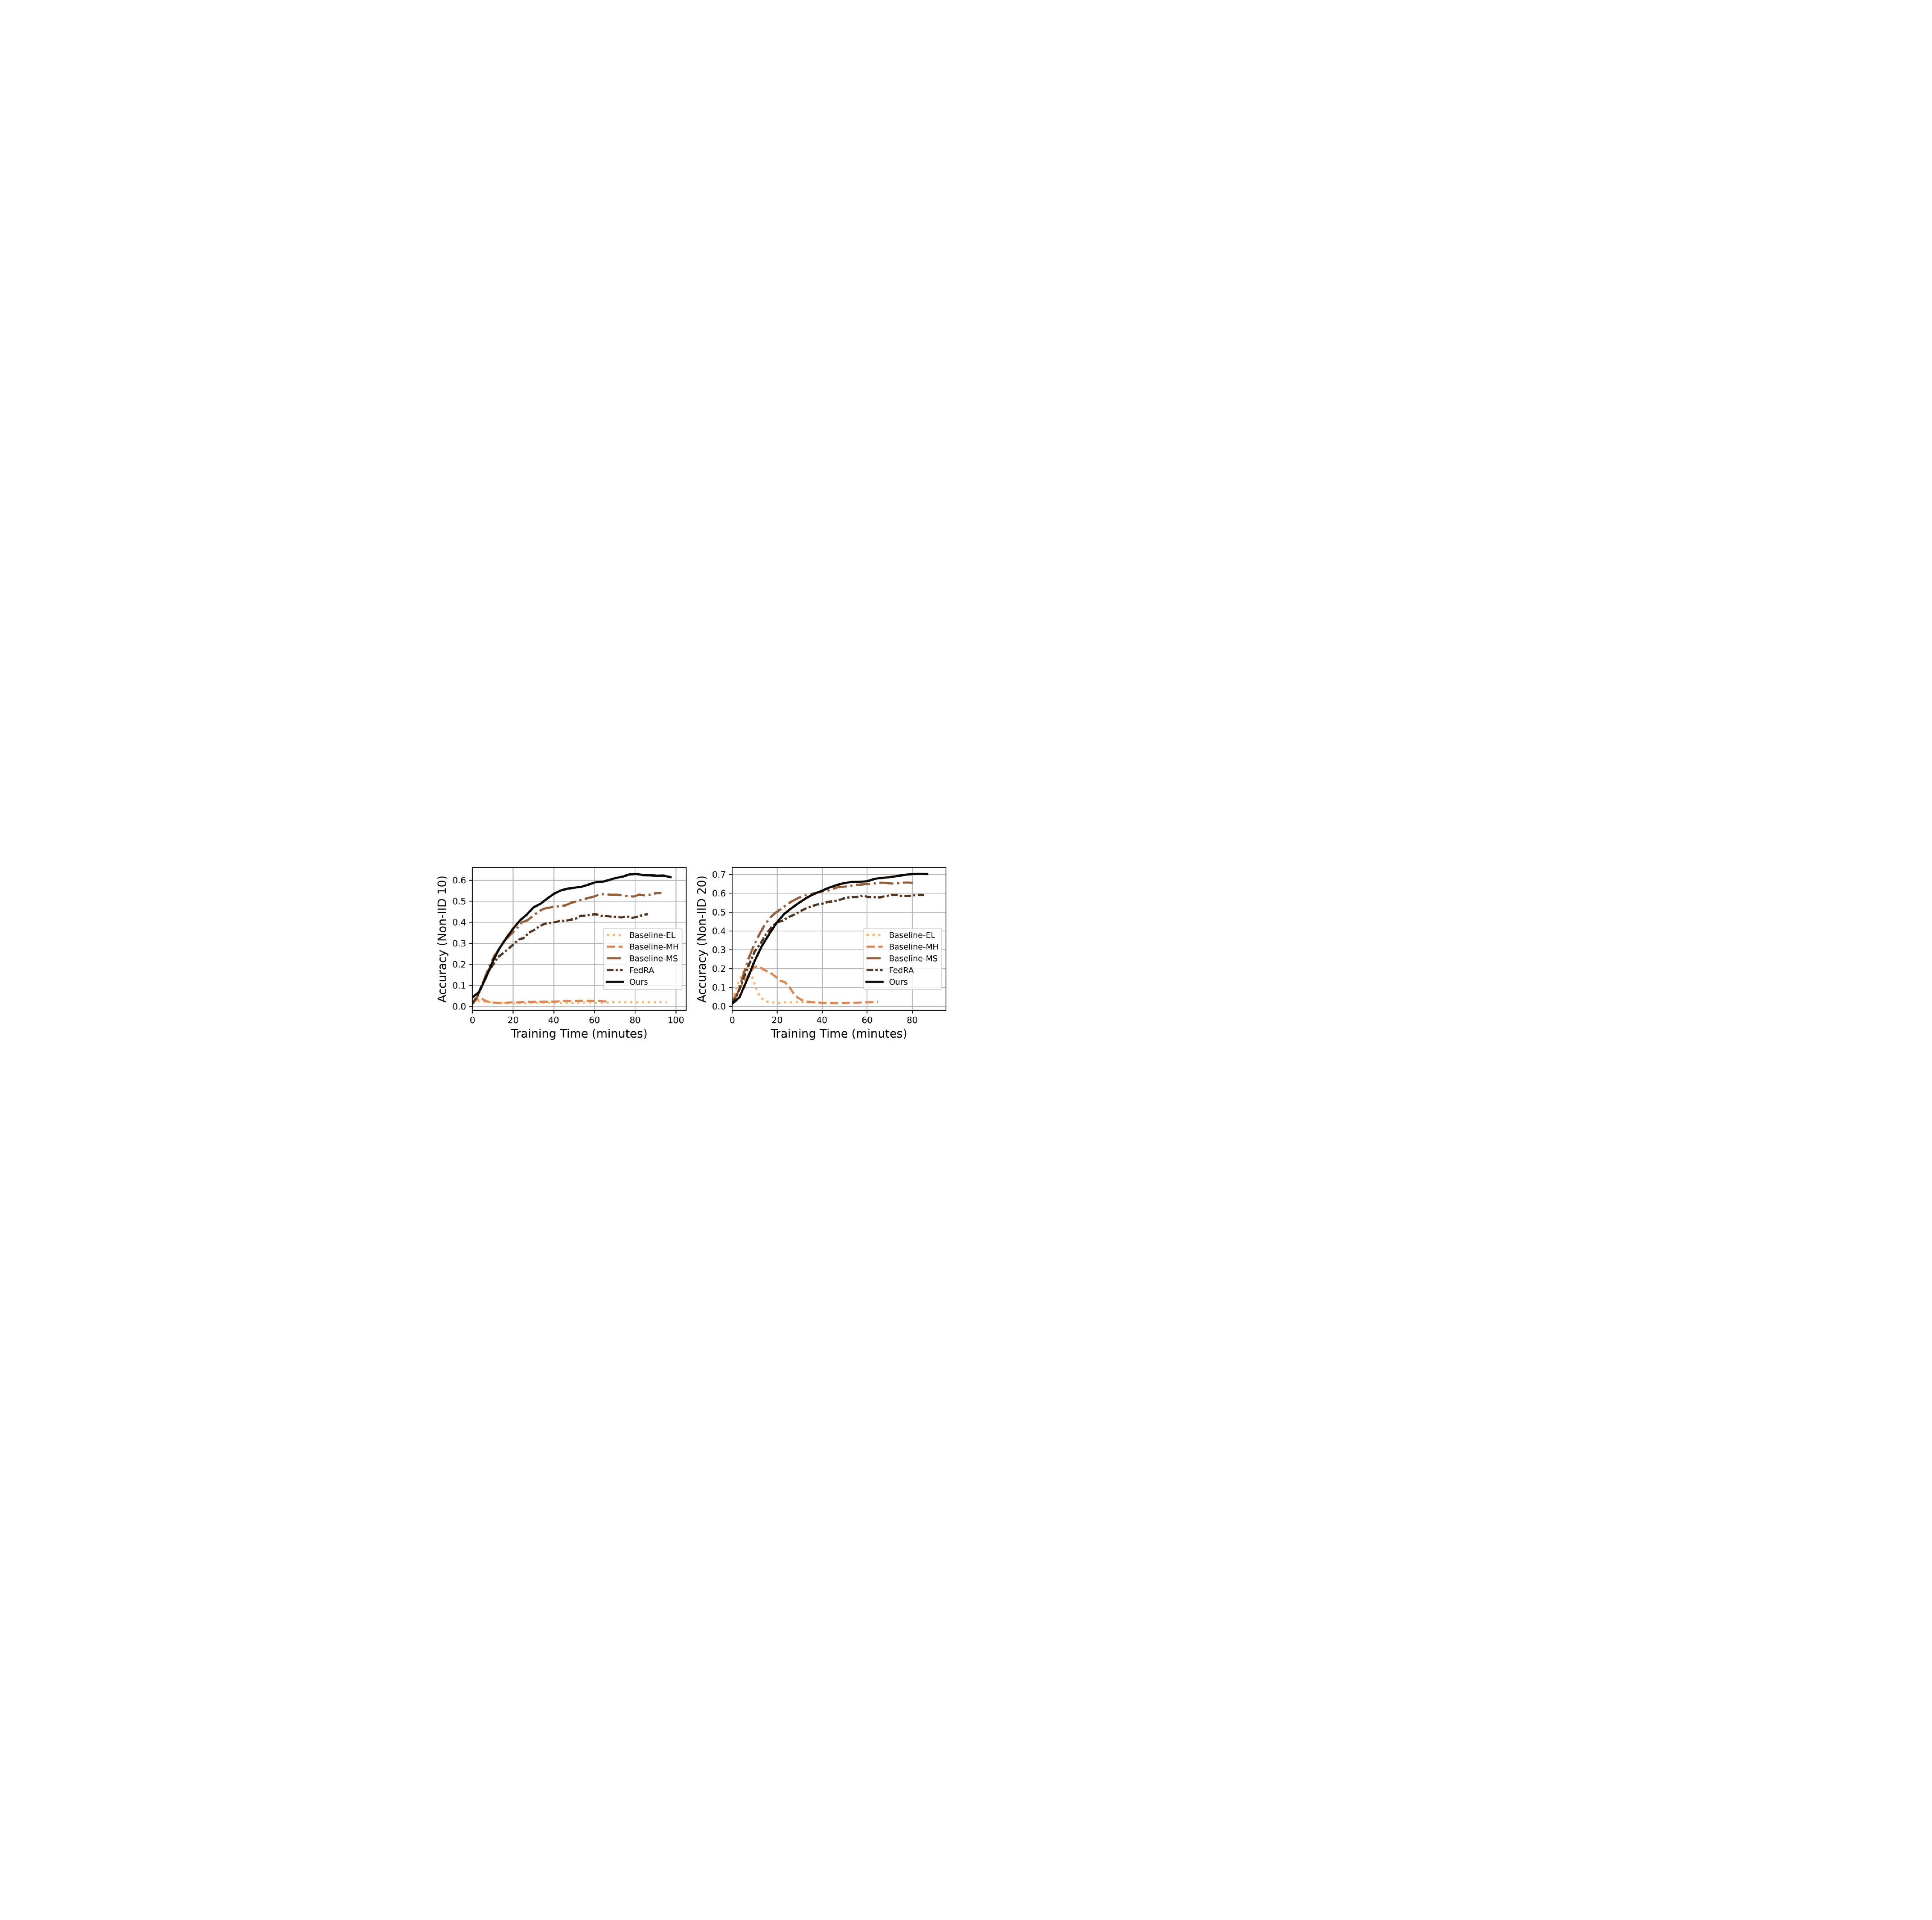
\includegraphics[width=0.45\textwidth]{fig/comp_eff.pdf}
% \vspace{-10pt}
\caption{Accuracy over training time on CIFAR-100 dataset (other methods not shown in the figure diverges).}
\label{fig:comp_eff}
\end{figure}

% Table generated by Excel2LaTeX from sheet 'Sheet2'
\begin{table}[t]
  \centering
    \caption{Ablation studies on IG score-based value function and aggregation rule ComAgg.}
    % \vskip 0.15in
    \scalebox{0.88}{
    \begin{tabular}{c|ccc}
    \toprule[1pt]
    \textbf{Methods}  & \textbf{IID} & \textbf{Non-IID (10)} & \textbf{Avg} \\
    \midrule
    Local IG score-based              & 75.81 & 58.80 & 67.30  \\
    Global IG score-based (using proxy data) & 79.74 & 63.17 & 71.45 \\ \midrule
    FedAvg & 75.86 & 57.35 & 66.60 \\
    ComAgg with $\alpha_{(j)}^t=\beta_{(j)}^t=1$ & 79.31 & 62.18 & 70.74 \\ \midrule
    \textbf{Ours}        & \cellcolor[rgb]{ .91,  .91,  .91}80.09 & \cellcolor[rgb]{ .91,  .91,  .91}63.93 & \cellcolor[rgb]{ .91,  .91,  .91}72.01 \\
    % \midrule
    % \midrule
    % ProxyData-IG-Score & \multicolumn{1}{c|}{\multirow{2}[2]{*}{\shortstack{LEDGAR\\BERT-base}}} & 62.61 & 47.35 & 54.98 \\
    % \textbf{Global-Local-IG-Score} &       & \cellcolor[rgb]{ .91,  .91,  .91}63.17 & \cellcolor[rgb]{ .91,  .91,  .91}48.87 & \cellcolor[rgb]{ .91,  .91,  .91}56.02 \\
    \bottomrule[1pt]
    \end{tabular}%
    }
    % \vspace{-11pt}
  \label{tab:ab1}%
  % \vskip -0.1in
\end{table}% 
% \vspace{-15pt}

\begin{table}[t]
  \centering
    \caption{The impact the number of total clients. Experiments are conducted on CIFAR-100 with Non-IID (10) settings. Accuracies are reported.}
    % \vskip 0.15in
    \scalebox{0.88}{
    \begin{tabular}{c|ccc}
    \toprule[1pt]
    \textbf{Method} &{\textbf{50}} &{\textbf{100}} &{\textbf{200}}  
    \\
    % \cline{1-1}
    \midrule
    Baseline-MS & 40.52 & 57.63 & 54.90 \\
    FedRA & 26.92 &47.98 & 44.90 \\
    Ours &\cellcolor[rgb]{ .91,  .91,  .91}59.46 & \cellcolor[rgb]{ .91,  .91,  .91}63.93 & \cellcolor[rgb]{ .91,  .91,  .91}63.50  \\
    \bottomrule[1pt]
    \end{tabular}%
    }
  \label{tab:sens-num-clients}%
  % \vskip -0.1in
\end{table}% 

% \textbf{IG-Score Evaluation.} 
To evaluate the effectiveness of our IG score-based value function, we conduct two ablation studies on CIFAR-100 dataset. We compare our value function with other alternations that only use the local IG score $I_i^t$ or a global IG score that is calculated using a proxy dataset sampled from the training data of clients. 

% First, we test the Local-only IG-Score.
% Second, we implement the ``global-only'' IG-Score using a proxy dataset sampled from the training data (size of $|D_{\text{IG}}|$) while ensuring no overlap with the training set.
% In each round of training, the server calculates the \textit{Global} IG-Score, which is subsequently downloaded by each selected client as the \textit{value} function for optimization. 
Table~\ref{tab:ab1} presents results under both IID and Non-IID (10) settings. Our method consistently outperforms others, improving over the Local IG Score-based strategy by +4.28\% and +5.13\% for IID and Non-IID, respectively. This highlights the necessity of global information. Our method also surpasses the Global IG Score-based method by +0.35\% (IID) and +0.76\% (Non-IID), demonstrating that proxy data alone is insufficient without local information.

% % Table generated by Excel2LaTeX from sheet 'Sheet3'
% \begin{table}[tbp]
%   \centering
%   \caption{Ablation Studies for Aggregation Rules on CIFAR-100 Dataset.}
%     \begin{tabular}{c|ccc}
%     \toprule[1pt]
%     \textbf{Methods/DH} & \textbf{IID} & \textbf{Non-IID} & \textbf{Avg} \\
%     \midrule
%     FedAvg & 75.86 & 57.35 & 66.60 \\
%     STAgg & 79.31 & 62.18 & 70.74 \\
%     \textbf{STAgg+DWA} & \cellcolor[rgb]{ .91,  .91,  .91}80.09 & \cellcolor[rgb]{ .91,  .91,  .91}63.93 & \cellcolor[rgb]{ .91,  .91,  .91}72.01 \\
%     \bottomrule[1pt]
%     \end{tabular}%
%   \label{tab:ab2}%
% \end{table}%

\textbf{Aggregation Rules Evaluation.} 
% We conduct ablation studies comparing our aggregation rules with FedAvg~\cite{mcmahan2017communication} and HAgg without dynamic weights $\alpha$ and $\beta$. As shown in Table~\ref{tab:ab1}, our method outperforms FedAvg by +4.23\% in IID and +6.58\% in non-IID settings. Additionally, the weighting strategy enhances STAgg by +1.27\% on average, highlighting the advantages of smoothed model updates.
We compare our aggregation rules with FedAvg~\cite{mcmahan2017communication} and ComAgg variant with coefficients $\alpha_{(j)}^t=\beta_{(j)}^t=1$. As shown in Table~\ref{tab:ab1}, our method outperforms FedAvg by +4.23\% in IID and +6.58\% in Non-IID settings. The dynamic compensation strategy further improves ComAgg by +1.27\% on average, demonstrating the benefits in mitigating model divergence.

\begin{table}[t]
\centering
\caption{The impacts of $T_{\text{IG}}$ and $T_{\text{Agg}}$. Experiments were conducted on CIFAR-100 under the Non-IID (10) setting. Each row varies one hyperparameter while fixing the other.}
\scalebox{0.88}{
\begin{tabular}{ccccc}
\toprule[1pt]
\textbf{Varying} & \textbf{Fixed Setting} & \textbf{5} & \textbf{10} & \textbf{20} \\
\hline
$T_{\text{IG}}$ & $T_{\text{Agg}}=10,\ |D_{\text{IG}}|=50$ & 63.15 & 63.93 & 62.93 \\
$T_{\text{Agg}}$ & $T_{\text{IG}}=10,\ |D_{\text{IG}}|=50$ & 63.24 & 63.93 & 63.41 \\
\bottomrule[1pt]
\end{tabular}
}
\label{tab:sens_tig_tagg}
\end{table}

\subsection{Impact of Hyperparameters}

We conduct experiments on CIFAR-100 dataset with the Non-IID (10) setting to evaluate the impact of hyperparameters such as the number of total clients, aggregation hyperparameters, and the size of the local IG dataset.

\textbf{The Number of Total Clients.} We keep the client sampling rate to 10\%, and vary the number of total clients to 50, 100, and 200. We only compare with Baseline-MS and FedRA, as other methods diverge in this Non-IID scenario. As shown in Table~\ref{tab:sens-num-clients}, our method consistently outperforms the baseline methods across all numbers of total client settings. 

\textbf{Hyperparameters $T_{\text{IG}}$ and $T_{\text{Agg}}$ for Aggregation.} Our default setting is $T_{\text{IG}}=$10 and $T_{\text{Agg}}=$10 . Varying $T_{\text{IG}}$ and $T_{\text{Agg}}$ show less than 1\% fluctuation in accuracy and consistently outperform other compared methods (compared in Table~\ref{tab:cifar100-results}). Nevertheless, we recommend selecting these hyperparameters based on the total number of clients and the client sampling rate.

\textbf{The size of local IG dataset $|D_{\text{IG}}|$.}
Our default setting uses $|D_{\text{IG}}| = 50$. As shown in Table~\ref{tab:sens-proxy-data-size}, reducing $|D_{\text{IG}}|$ to 5 or 10 results in only minor performance fluctuations, demonstrating that our method places minimal requirements on the size of the IG dataset. Since the IG scores are primarily used for model calibration, our method generalizes well even when clients have a limited amount of local data.

% \begin{table}[t]
%   \centering
%     \caption{The memory utilization of three levels of resource-constraint clients with Data-Juicer model and Fed-pilot.}
%     % \vskip 0.15in
%     \scalebox{0.95}{
%     \begin{tabular}{cc}
%     \toprule[1pt]
    
%     \textbf{Memory Cost Ratio (\%)} &{\textbf{Memory Cost (GB)}}  
%     \\
%     % \cline{1-1}
%     \midrule
% \progressbar{98.78}/\progressbar{99.22}/\progressbar{97.66} & 31.61 / 39.68 / 46.87 \\
%     \bottomrule[1pt]
%     \end{tabular}%
%     }
%   \label{tab:memory_utilization}%
%   % \vskip -0.1in
% \end{table}% 

% \begin{table}[t]
% \centering
% \caption{Communication cost (MB) comparison across methods on the NI dataset.}
% \begin{tabular}{cccc}
% \toprule[1pt]
% \textbf{Method} & \textbf{Total} &\textbf{Uplink} & \textbf{Downlink} \\
% \hline
% Baseline-EL   & 6.92 \\
% Baseline-MH   & 6.97 \\
% Baseline-MS   & 10.70 \\ \midrule
% FLoRA         & 12.05 \\
% FlexLoRA      &       \\
% HETLoRA       & 11.43 \\
% FedRA         & 12.87 \\ \midrule
% Ours          & 10.58 \\
% \bottomrule[1pt]
% \end{tabular}
% \label{tab:comm_cost}
% \end{table}



\begin{figure}[t]
\centering
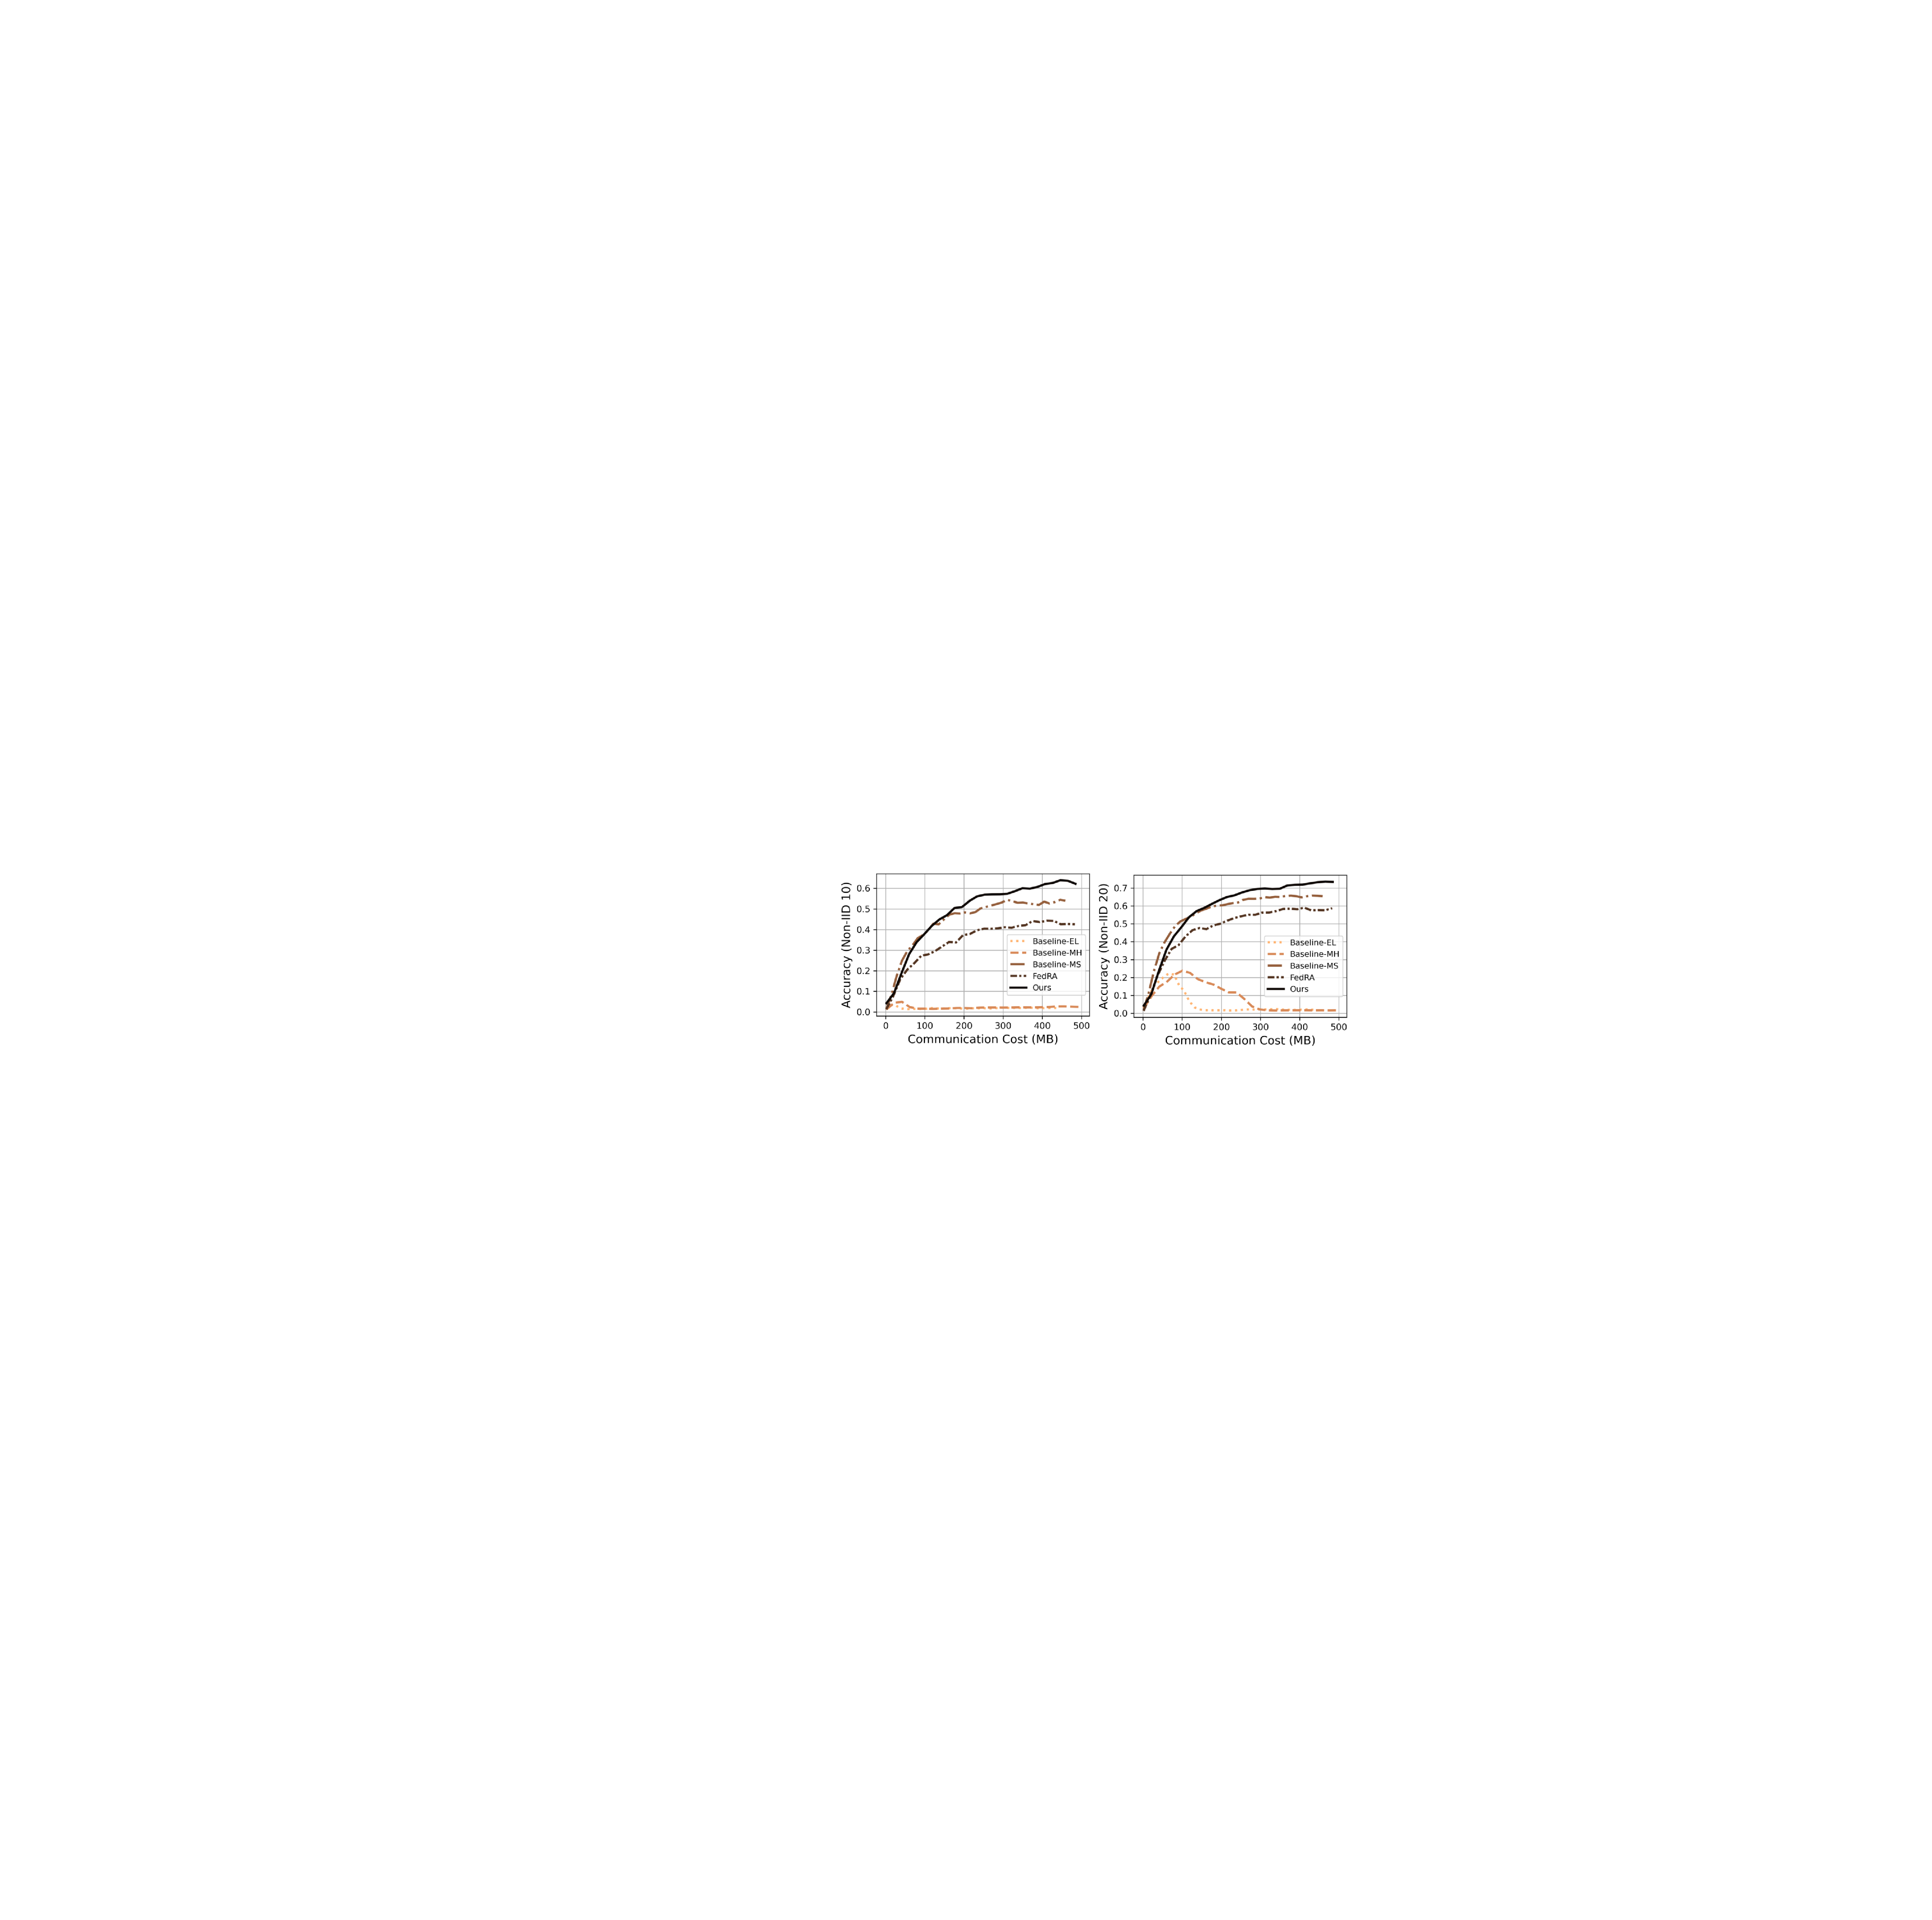
\includegraphics[width=0.45\textwidth]{fig/comm_eff.pdf}
% \vspace{-10pt}
\caption{Accuracy over communication cost on CIFAR-100 dataset (other methods not shown in the figure diverged).}
\label{fig:comm_eff}
\end{figure}

\begin{table}[t]
\centering
\caption{The impact of the size of local IG dataset $|D_{\text{IG}}|$. Experiments are conducted on CIFAR-100 under the Non-IID (10) setting.}
\scalebox{0.88}{
\begin{tabular}{cccc}
\toprule[1pt]
\textbf{Fixed Setting} & \textbf{5} & \textbf{10} & \textbf{50} \\
\hline
$T_{\text{Agg}}=10,\ T_{\text{IG}}=10$ & 62.78 & 62.60 & 62.93 \\
\bottomrule[1pt]
\end{tabular}
}
\label{tab:sens-proxy-data-size}
\end{table}

\subsection{Computation and Communication Efficiency}

We evaluate the computational and communication efficiency of our method by observing model accuracy over the cumulative training time and total communication cost during training, respectively. Compared to FedAvg, our method introduces additional computational cost every $T_{\text{IG}}$ rounds for optimizing the LoRA allocation, but reduces communication costs for low-resource clients by transmitting fewer parameters. 
%We apply exponential moving average smoothing with a decay factor of 0.9 to the raw accuracy values for better comparison.

\textbf{Computational Efficiency.} Figure~\ref{fig:comp_eff} presents the accuracy over training time for all methods on the Non-IID CIFAR-100 dataset. In this case, our method consistently achieves higher accuracy within the same training time (i.e., wall-clock time). Specifically, Baseline-EL and Baseline-MH diverge under the extreme Non-IID setting due to the lack of data from all the clients. Baseline-MS and FedRA do not incur additional computational costs compared to FedAvg, and therefore exhibit higher computational efficiency in the early stages (as shown in Figure~\ref{fig:comp_eff}, Non-IID 20). However, they suffer from accuracy degradation compared to our method due to their reliance on heuristic or stochastic LoRA allocation strategies. Although our method periodically incurs additional computational costs for LoRA allocation optimization, its accuracy gains lead to higher overall computational efficiency. 

% In contrast, our method considers the varying contributions of different LoRA modules, resulting in higher computational efficiency.

\textbf{Communication Efficiency.} 
Figure~\ref{fig:comm_eff} presents the accuracy over communication cost for all methods on the Non-IID CIFAR-100 dataset.
% To analyze communication efficiency, we report accuracy versus communication cost, as shown in Figure~\ref{fig:comm_eff}. 
We calculate both uplink and downlink communication costs per client during the training. Baseline-EL and Baseline-MH diverge but still incur a large amount of communication cost. FedRA and Baseline-MS both select a subset of LoRA modules to update locally, which also helps reduce the uplink communication costs for low-resource clients.  
% 
Baseline-MS shows slightly higher computational efficiency in the early stages, as it enables more layers to be trained under the same memory constraint compared to FedRA and our method, leading to faster initial convergence.
%as the model converges faster with more LoRA modules in the early stage. 
However, this benefit diminishes over time, as it restricts training to only the last few layers, leaving the earlier layers untouched, which ultimately results in lower communication efficiency compared to our method. Overall, our method achieves a better trade-off between model accuracy and communication cost.

\section{Conclusion}\label{conclusion}
This paper presents Fed-pilot, a novel framework for optimizing LoRA allocation in federated fine-tuning while considering clients' memory capacities. We introduce the IG score to quantify each LoRA module's importance and design the optimization process that maximizes global model performance under heterogeneous memory constraints. Additionally, we develop a novel aggregation rule to handle diverse model updates under optimal LoRA allocation. Evaluations on five distinct FM fine-tuning tasks demonstrate the effectiveness and efficiency of Fed-pilot.




% \section{Acknowledgments}

% % Identification of funding sources and other support, and thanks to
% % individuals and groups that assisted in the research and the
% % preparation of the work should be included in an acknowledgment
% % section, which is placed just before the reference section in your
% % document.

% This section has a special environment:
% \begin{verbatim}
%   \begin{acks}
%   ...
%   \end{acks}
% \end{verbatim}
% so that the information contained therein can be more easily collected
% during the article metadata extraction phase, and to ensure
% consistency in the spelling of the section heading.

% Authors should not prepare this section as a numbered or unnumbered {\verb|\section|}; please use the ``{\verb|acks|}'' environment.

% \section{Appendices}

% If your work needs an appendix, add it before the
% ``\verb|\end{document}|'' command at the conclusion of your source
% document.

% Start the appendix with the ``\verb|appendix|'' command:
% \begin{verbatim}
%   \appendix
% \end{verbatim}
% and note that in the appendix, sections are lettered, not
% numbered. This document has two appendices, demonstrating the section
% and subsection identification method.

% \section{Multi-language papers}

% Papers may be written in languages other than English or include
% titles, subtitles, keywords and abstracts in different languages (as a
% rule, a paper in a language other than English should include an
% English title and an English abstract).  Use \verb|language=...| for
% every language used in the paper.  The last language indicated is the
% main language of the paper.  For example, a French paper with
% additional titles and abstracts in English and German may start with
% the following command
% \begin{verbatim}
% \documentclass[sigconf, language=english, language=german,
%                language=french]{acmart}
% \end{verbatim}

% The title, subtitle, keywords and abstract will be typeset in the main
% language of the paper.  The commands \verb|\translatedXXX|, \verb|XXX|
% begin title, subtitle and keywords, can be used to set these elements
% in the other languages.  The environment \verb|translatedabstract| is
% used to set the translation of the abstract.  These commands and
% environment have a mandatory first argument: the language of the
% second argument.  See \verb|sample-sigconf-i13n.tex| file for examples
% of their usage.

% \section{SIGCHI Extended Abstracts}

% The ``\verb|sigchi-a|'' template style (available only in \LaTeX\ and
% not in Word) produces a landscape-orientation formatted article, with
% a wide left margin. Three environments are available for use with the
% ``\verb|sigchi-a|'' template style, and produce formatted output in
% the margin:
% \begin{description}
% \item[\texttt{sidebar}:]  Place formatted text in the margin.
% \item[\texttt{marginfigure}:] Place a figure in the margin.
% \item[\texttt{margintable}:] Place a table in the margin.
% \end{description}

%%
%% The acknowledgments section is defined using the "acks" environment
%% (and NOT an unnumbered section). This ensures the proper
%% identification of the section in the article metadata, and the
%% consistent spelling of the heading.
% \begin{acks}
% To Robert, for the bagels and explaining CMYK and color spaces.
% \end{acks}

%%
%% The next two lines define the bibliography style to be used, and
%% the bibliography file.
\bibliographystyle{ACM-Reference-Format}
\bibliography{main}


%%
%% If your work has an appendix, this is the place to put it.
% \appendix

% \section{Research Methods}

% \subsection{Part One}

% Lorem ipsum dolor sit amet, consectetur adipiscing elit. Morbi
% malesuada, quam in pulvinar varius, metus nunc fermentum urna, id
% sollicitudin purus odio sit amet enim. Aliquam ullamcorper eu ipsum
% vel mollis. Curabitur quis dictum nisl. Phasellus vel semper risus, et
% lacinia dolor. Integer ultricies commodo sem nec semper.

% \subsection{Part Two}

% Etiam commodo feugiat nisl pulvinar pellentesque. Etiam auctor sodales
% ligula, non varius nibh pulvinar semper. Suspendisse nec lectus non
% ipsum convallis congue hendrerit vitae sapien. Donec at laoreet
% eros. Vivamus non purus placerat, scelerisque diam eu, cursus
% ante. Etiam aliquam tortor auctor efficitur mattis.

% \section{Online Resources}

% Nam id fermentum dui. Suspendisse sagittis tortor a nulla mollis, in
% pulvinar ex pretium. Sed interdum orci quis metus euismod, et sagittis
% enim maximus. Vestibulum gravida massa ut felis suscipit
% congue. Quisque mattis elit a risus ultrices commodo venenatis eget
% dui. Etiam sagittis eleifend elementum.

% Nam interdum magna at lectus dignissim, ac dignissim lorem
% rhoncus. Maecenas eu arcu ac neque placerat aliquam. Nunc pulvinar
% massa et mattis lacinia.

%%%%%%%%%%%%%%%%%%%%%%%%%%%%%%%%%%%%%%%%%%%%%%%%%%%%%%%%%%%%%%%%%%%%%%%%%%%%%%%
%%%%%%%%%%%%%%%%%%%%%%%%%%%%%%%%%%%%%%%%%%%%%%%%%%%%%%%%%%%%%%%%%%%%%%%%%%%%%%%
% APPENDIX
%%%%%%%%%%%%%%%%%%%%%%%%%%%%%%%%%%%%%%%%%%%%%%%%%%%%%%%%%%%%%%%%%%%%%%%%%%%%%%%
%%%%%%%%%%%%%%%%%%%%%%%%%%%%%%%%%%%%%%%%%%%%%%%%%%%%%%%%%%%%%%%%%%%%%%%%%%%%%%%
\newpage
\appendix
\onecolumn
% \setcounter{equation}{0}
\setcounter{page}{1}
% \setcounter{figure}{0}
% \setcounter{table}{0}


\section*{Supplement}

We provide more discussions and experiments of this work in the supplement and organize it as follows:

\begin{itemize}
    \item Supplement~\ref{sec:appendix-gpu-memory-consumption}: Additional details on memory consumption in LoRA-based FM fine-tuning.
        \begin{itemize}
            \item In Subsection~\ref{subsec:appendix-dynamic-activation}, we provide an example of how to calculate activations with only a frozen linear layer.
            \item In Subsection~\ref{subsec:appendix-static-activation}, we provide an example of how to calculate activations with a frozen non-linear layer.
            \item In Subsection~\ref{subsec:appendix-dynamic-static-activation}, we provide details on the type of activation in the ViT model.
            \item In Subsection~\ref{subsec:appendix-memory-footprint-example}, we provide a code of how to calculate memory consumption for a given LoRA allocation map with ViT-base.
        \end{itemize}

    % \item Supplement~\ref{sec:appendix-algorithm}: The algorithm details of Fed-piLot.
    
    \item Supplement~\ref{sec:appendix-settings}: We provide detailed information on the experimental settings, including the models, FL settings, GPU memory capacity configurations for each client and model level, the resources and infrastructure used for the experiments, and a detailed explanation of the experiments shown in Figure~\ref{fig:motivation}.
        \begin{itemize}
            \item In Subsection~\ref{subsec:appendix-settings-flsettings}, we outline the FL-related settings and hyperparameters.
            \item In Subsection~\ref{subsec:appendix-capacity-settings}, we describe the capacity chooses for each model.
            \item In Subsection~\ref{subsec:appendix-motivation-settings}, we provide a detailed explanation of the experimental settings used for Figure~\ref{fig:motivation}.
        \end{itemize}
   
    \item Supplement~\ref{sec:appendix-dataset}: Details on the preprocessing of all datasets are provided.

    \item Supplement~\ref{sec:appendix-results-visualization}: Additional results are presented in tables.
    
    \item Supplement~\ref{sec:appendix-comparative_study}: A comparative study on state-of-the-art methods is provided.

    \item Supplement~\ref{sec:appendix-limitation}: The limitations of our work are discussed.
   
    \item Supplement~\ref{sec:appendix-futurework}: Directions for future work are outlined.

\end{itemize}



% \section{The Convergence Curve}\label{sec:appendix-convergence-curve}

% \section{The Convergence Analysis}\label{sec:appendix-convergence-analysis}

\section{GPU Memory Consumption of Model Fine-Tuning with LoRA}\label{sec:appendix-gpu-memory-consumption}

    \subsection{Backpropagation for Linear Layers: Saving Dynamic Activation using Freezing}\label{subsec:appendix-dynamic-activation}
    
    We provide a simple example~\cite{ardakani2024slimfit} demonstrating how gradients are backpropagated to the first layer of a neural network while its middle layer is frozen. To this end, let us perform backpropagation using a 3-layer neural network as an example. The architecture of this network is described as follows,
    
    \begin{align}
        \mathbf{y}_1 &= \mathbf{x}\mathbf{W}_1 + \mathbf{b}_1, \\
        \mathbf{y}_2 &= \mathbf{y}_1\mathbf{W}_2 + \mathbf{b}_2, \\
        \mathbf{y}_3 &= \mathbf{y}_2\mathbf{W}_3 + \mathbf{b}_3.
    \end{align}
    
    where $\{\mathbf{W}_1, \mathbf{W}_2, \mathbf{W}_3$\} and $\{\mathbf{b}_1, \mathbf{b}_2, \mathbf{b}_3\}$ are the weights and biases of the network, respectively. In this example, $\mathbf{x}$, $\mathbf{y}_1$, and $\mathbf{y}_2$ are input to the first layer, the second layer, and the third layer, respectively. 
    The backpropagation equations for the loss $\mathcal{L}$ using the chain rule can be presented as follows,
    
    \begin{align}
        \frac{\partial \mathcal{L}}{\partial \mathbf{W}_3} &= \frac{\partial \mathcal{L}}{\partial \mathbf{y}_3} \frac{\partial \mathbf{y}_3}{\partial \mathbf{W}_3} = \frac{\partial \mathcal{L}}{\partial \mathbf{y}_3} \mathbf{y}_2, \\
        \frac{\partial \mathcal{L}}{\partial \mathbf{b}_3} &= \frac{\partial \mathcal{L}}{\partial \mathbf{y}_3} \frac{\partial \mathbf{y}_3}{\partial \mathbf{b}_3} = \frac{\partial \mathcal{L}}{\partial \mathbf{y}_3}, \\
        \frac{\partial \mathcal{L}}{\partial \mathbf{W}_2} &= \frac{\partial \mathcal{L}}{\partial \mathbf{y}_3} \frac{\partial \mathbf{y}_3}{\partial \mathbf{y}_2} \frac{\partial \mathbf{y}_2}{\partial \mathbf{W}_2} = \frac{\partial \mathcal{L}}{\partial \mathbf{y}_3} \mathbf{W}_3^\top \mathbf{y}_1, \\
        \frac{\partial \mathcal{L}}{\partial \mathbf{b}_2} &= \frac{\partial \mathcal{L}}{\partial \mathbf{y}_3} \frac{\partial \mathbf{y}_3}{\partial \mathbf{y}_2} \frac{\partial \mathbf{y}_2}{\partial \mathbf{b}_2} = \frac{\partial \mathcal{L}}{\partial \mathbf{y}_3} \mathbf{W}_3^\top, \\
        \frac{\partial \mathcal{L}}{\partial \mathbf{W}_1} &= \frac{\partial \mathcal{L}}{\partial \mathbf{y}_3} \frac{\partial \mathbf{y}_3}{\partial \mathbf{y}_2} \frac{\partial \mathbf{y}_2}{\partial \mathbf{y}_1} \frac{\partial \mathbf{y}_1}{\partial \mathbf{W}_1} = \frac{\partial \mathcal{L}}{\partial \mathbf{y}_3} \mathbf{W}_3^\top \mathbf{W}_2^\top \mathbf{x}, \\
        \frac{\partial \mathcal{L}}{\partial \mathbf{b}_1} &= \frac{\partial \mathcal{L}}{\partial \mathbf{y}_3} \frac{\partial \mathbf{y}_3}{\partial \mathbf{y}_2} \frac{\partial \mathbf{y}_2}{\partial \mathbf{y}_1} \frac{\partial \mathbf{y}_1}{\partial \mathbf{b}_1} = \frac{\partial \mathcal{L}}{\partial \mathbf{y}_3} \mathbf{W}_3^\top \mathbf{W}_2^\top.
    \end{align}

    where $\partial$ denotes the partial derivative, and $\frac{\partial \mathcal{L}}{\partial \mathbf{W}_3}$ is obtained by computing the loss.
    
    \textbf{Training all three layers.} To update all the network weights (i.e., $\mathbf{W}_1, \mathbf{W}_2, \mathbf{W}_3$), we need to store $\mathbf{x}$, $\mathbf{y}_1$, and $\mathbf{y}_2$ during forward computations, as they are required in the gradient calculations.
    
    \textbf{Training two layers while freezing the middle layer.} In the case of freezing the middle layer, it is unnecessary to compute the gradient update for $\mathbf{W}_2$:
    
    \begin{equation}
        \frac{\partial \mathcal{L}}{\partial \mathbf{W}_2} = \frac{\partial \mathcal{L}}{\partial \mathbf{y}_3} \mathbf{W}_3^\top \mathbf{y}_1.
    \end{equation}
    
    Therefore, there is no need to store $\mathbf{y}_1$ during the forward pass. However, discarding $\mathbf{y}_1$ does not affect the backward computations of the first layer, since the updates for $\mathbf{W}_1$ and $\mathbf{b}_1$ are independent of $\mathbf{y}_1$:
    
    \begin{align}
        \frac{\partial \mathcal{L}}{\partial \mathbf{W}_1} &= \frac{\partial \mathcal{L}}{\partial \mathbf{y}_3} \mathbf{W}_3^\top \mathbf{W}_2^\top \mathbf{x}, \\
        \frac{\partial \mathcal{L}}{\partial \mathbf{b}_1} &= \frac{\partial \mathcal{L}}{\partial \mathbf{y}_3} \mathbf{W}_3^\top \mathbf{W}_2^\top \mathbf{1}.
    \end{align}
    
    This example illustrates how freezing an intermediate linear layer affects the backpropagation process. For a liner layer, activation can be discarded if the layer is frozen.

    \subsection{Backpropagation for Non-Linear Layers: Static Activation Remains using Freezing
    }\label{subsec:appendix-static-activation}

    
    Here, we demonstrate how non-linear transformations (such as Softmax, GELU, and LayerNorm) impact backpropagation in a 3-layer neural network. By extending the example in~\cite{ardakani2024slimfit}, the architecture of the network is defined as follows:

    % We provide a simple example demonstrating how gradients are backpropagated to the first layer of a neural network while its middle layer is a non-linear transformation. To this end, let us perform backpropagation using a 3-layer neural network as an example. The architecture of this network is described as follows,
    
    \begin{align}
        \mathbf{y}_1 &= \mathbf{x}\mathbf{W}_1 + \mathbf{b}_1, \\
        \mathbf{y}_2 &= \sigma(\mathbf{y}_1\mathbf{W}_2 + \mathbf{b}_2), \\
        \mathbf{y}_3 &= \mathbf{y}_2\mathbf{W}_3 + \mathbf{b}_3.
    \end{align}
    
    where $\{\mathbf{W}_1, \mathbf{W}_2, \mathbf{W}_3\}$ and $\{\mathbf{b}_1, \mathbf{b}_2, \mathbf{b}_3\}$ are the weights and biases of the network, respectively. In this example, $\mathbf{x}$, $\mathbf{y}_1$, and $\mathbf{y}_2$ are input to the first layer, the second layer, and the third layer, respectively. The non-linear function $\sigma(\cdot)$ introduces non-linearity in the second layer. The backpropagation equations for the loss $\mathcal{L}$ using the chain rule can be presented as follows,
    
    \begin{align}
        \frac{\partial \mathcal{L}}{\partial \mathbf{W}_3} &= \frac{\partial \mathcal{L}}{\partial \mathbf{y}_3} \frac{\partial \mathbf{y}_3}{\partial \mathbf{W}_3} = \frac{\partial \mathcal{L}}{\partial \mathbf{y}_3} \mathbf{y}_2, \\
        \frac{\partial \mathcal{L}}{\partial \mathbf{b}_3} &= \frac{\partial \mathcal{L}}{\partial \mathbf{y}_3} \frac{\partial \mathbf{y}_3}{\partial \mathbf{b}_3} = \frac{\partial \mathcal{L}}{\partial \mathbf{y}_3}, \\
        \frac{\partial \mathcal{L}}{\partial \mathbf{W}_2} &= \frac{\partial \mathcal{L}}{\partial \mathbf{y}_3} \frac{\partial \mathbf{y}_3}{\partial \mathbf{y}_2} \frac{\partial \mathbf{y}_2}{\partial \mathbf{W}_2} = \frac{\partial \mathcal{L}}{\partial \mathbf{y}_3} \mathbf{W}_3^\top \sigma'(\mathbf{y}_1\mathbf{W}_2 + \mathbf{b}_2) \mathbf{y}_1, \\
        \frac{\partial \mathcal{L}}{\partial \mathbf{b}_2} &= \frac{\partial \mathcal{L}}{\partial \mathbf{y}_3} \frac{\partial \mathbf{y}_3}{\partial \mathbf{y}_2} \frac{\partial \mathbf{y}_2}{\partial \mathbf{b}_2} = \frac{\partial \mathcal{L}}{\partial \mathbf{y}_3} \mathbf{W}_3^\top \sigma'(\mathbf{y}_1\mathbf{W}_2 + \mathbf{b}_2), \\
        \frac{\partial \mathcal{L}}{\partial \mathbf{W}_1} &= \frac{\partial \mathcal{L}}{\partial \mathbf{y}_3} \frac{\partial \mathcal{L}}{\partial \mathbf{y}_3}{\partial \mathbf{y}_2} \frac{\partial \mathbf{y}_2}{\partial \mathbf{y}_1} \frac{\partial \mathbf{y}_1}{\partial \mathbf{W}_1} = \frac{\partial \mathcal{L}}{\partial \mathbf{y}_3} \mathbf{W}_3^\top \sigma'(\mathbf{y}_1\mathbf{W}_2 + \mathbf{b}_2) \mathbf{W}_2^\top \mathbf{x}, \\
        \frac{\partial \mathcal{L}}{\partial \mathbf{b}_1} &= \frac{\partial \mathcal{L}}{\partial \mathbf{y}_3} \frac{\partial \mathcal{L}}{\partial \mathbf{y}_3}{\partial \mathbf{y}_2} \frac{\partial \mathbf{y}_2}{\partial \mathbf{y}_1} \frac{\partial \mathbf{y}_1}{\partial \mathbf{b}_1} = \frac{\partial \mathcal{L}}{\partial \mathbf{y}_3} \mathbf{W}_3^\top \sigma'(\mathbf{y}_1\mathbf{W}_2 + \mathbf{b}_2) \mathbf{W}_2^\top.
    \end{align}
    % where $\partial$ denotes the partial derivative, and $\frac{\partial \mathcal{L}}{\partial \mathbf{W}_3}$ is obtained by computing the loss. 
    Here, $\sigma^{\prime}(\mathbf{y}_1\mathbf{W}_2)$ represents the derivative of the non-linear function $\sigma(\cdot)$ applied to the linear transformation $\mathbf{y}_1\mathbf{W}_2 + \mathbf{b}_2$.
    
    \textbf{Training all three layers.} To update all the network weights (i.e., $\mathbf{W}_1, \mathbf{W}_2, \mathbf{W}_3$), we need to store $\mathbf{x}$, $\mathbf{y}_1$, and $\mathbf{y}_2$ during forward computations, as they are required in the gradient calculations.
    
    \textbf{Training two layers while freezing the middle layer.} In the case of freezing the middle layer, it is unnecessary to compute the gradient update for $\mathbf{W}_2$:

    \begin{equation}
        \frac{\partial \mathcal{L}}{\partial \mathbf{W}_2} = \frac{\partial \mathcal{L}}{\partial \mathbf{y}_3} \mathbf{W}_3^\top \sigma'(\mathbf{y}_1\mathbf{W}_2 + \mathbf{b}_2) \mathbf{y}_1.
    \end{equation}

    However, unlike the linear case, it is \textbf{necessary} to store $\mathbf{y}_1$ during the forward pass because the gradients for $\mathbf{w}_1$ and $\mathbf{b}_1$ depends on $\sigma'(\mathbf{y}_1\mathbf{W}_2 + \mathbf{b}_2)$. Discarding $\mathbf{y}_1$ would prevent the correct computation of gradients for $\mathbf{W}_1$ and $\mathbf{b}_1$, as their updates explicitly involve $\mathbf{y}_1$:

    \begin{align}
        \frac{\partial \mathcal{L}}{\partial \mathbf{W}_1} &= \frac{\partial \mathcal{L}}{\partial \mathbf{y}_3} \mathbf{W}_3^\top \sigma'(\mathbf{y}_1\mathbf{W}_2 + \mathbf{b}_2) \mathbf{W}_2^\top \mathbf{x}, \\
        \frac{\partial \mathcal{L}}{\partial \mathbf{b}_1} &= \frac{\partial \mathcal{L}}{\partial \mathbf{y}_3} \mathbf{W}_3^\top \sigma'(\mathbf{y}_1\mathbf{W}_2 + \mathbf{b}_2) \mathbf{W}_2^\top.
    \end{align}

    This example illustrates how freezing an intermediate non-linear layer affects the backpropagation process. Unlike the linear case, where activations can be discarded when a layer is frozen, a non-linear layer requires storing its activations due to its role in computing the gradients of earlier layers.

    \begin{figure}[t]
    \centering
    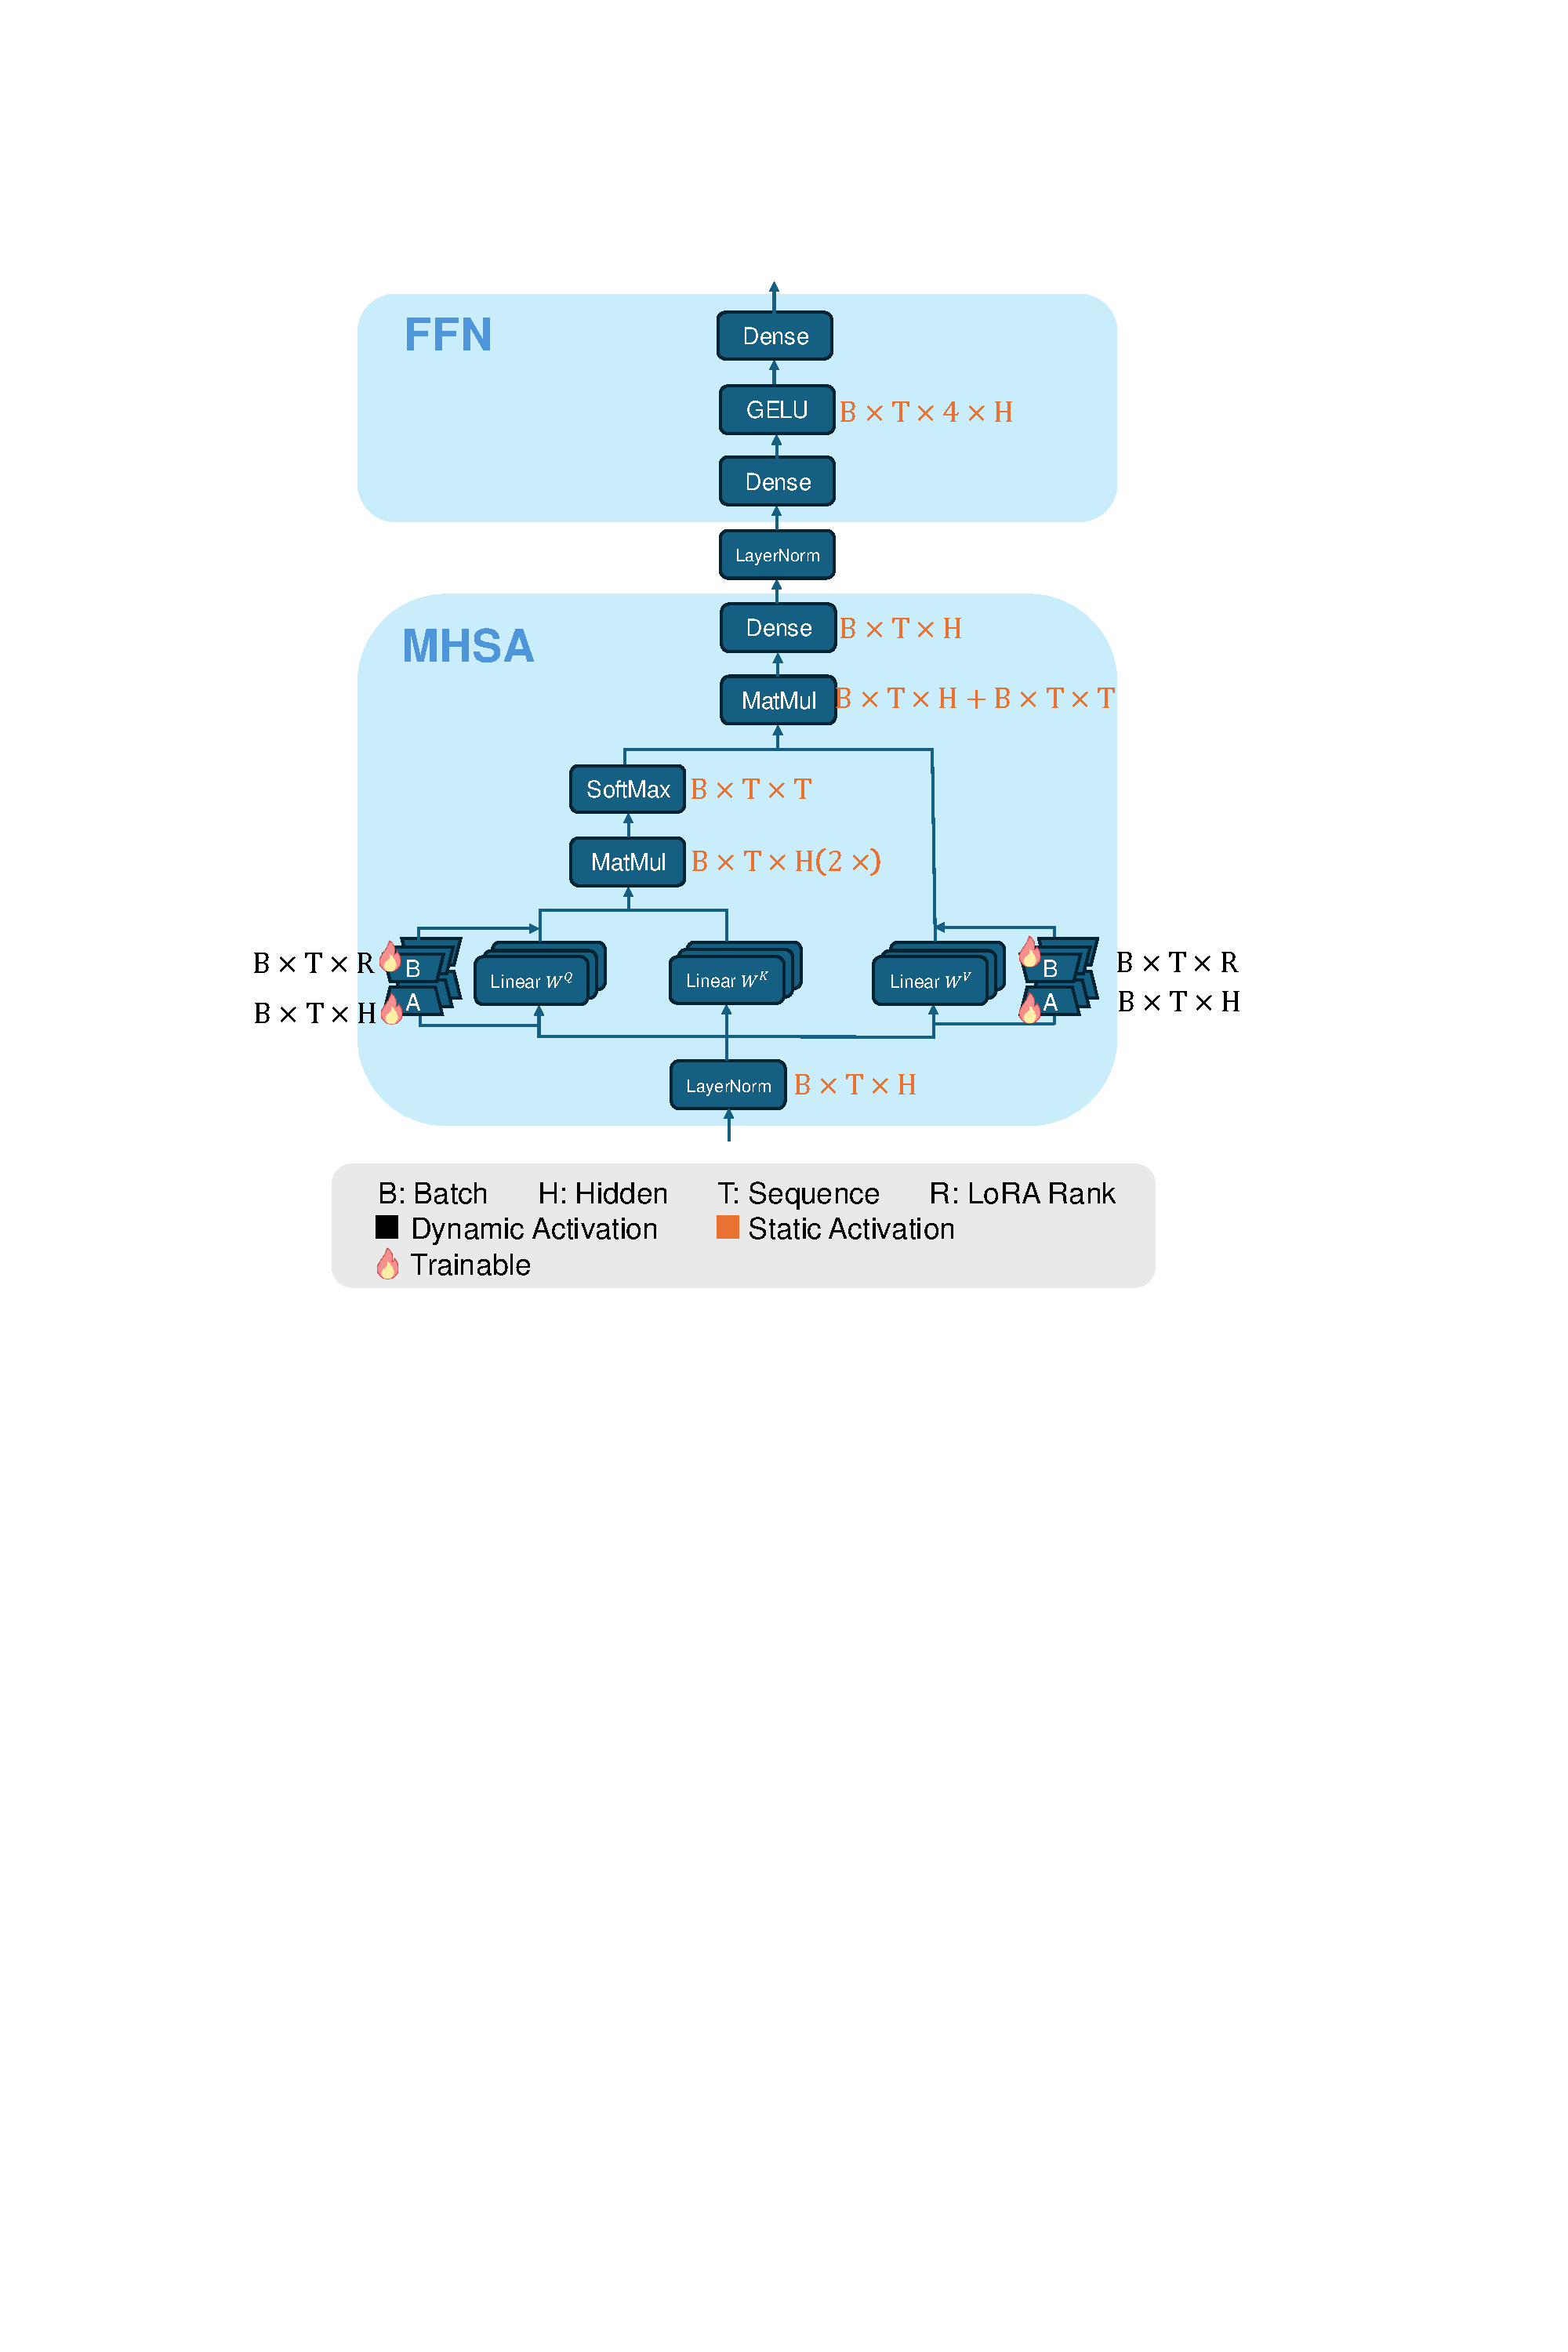
\includegraphics[width=0.45\textwidth]{fig/memorycost.pdf}
    % \vspace{-10pt}
    \caption{Illustration of activation memory usage in a transformer block for the ViT-base model (the rest layers are frozen if not specified.}
    \label{fig:memorycost}
    \end{figure}

    \subsection{Dynamic and Static Activations: An Example for ViT-base with LoRA module}\label{subsec:appendix-dynamic-static-activation}

    \begin{table}[t]
    \centering
    \caption{Details of transformer block of for ViT-base, including the internal layer types, descriptions, activation sizes, and type of activations~\cite{ardakani2024slimfit}.}
    \caption{Memory consumption estimates for training different LoRA modules.}
    \scalebox{1.2}{
    \begin{tabular}{c|c|c|c|c}
    \toprule[1pt]
    \textbf{Module} & \textbf{Type of Layer} & \textbf{Description} & \textbf{\# Activations}  & \textbf{Type of Activations}\\ \hline
    \multirow{8}{*}{MHSA} 
        & Dense     & attention.query    & $B \times T \times H$ & Dynamic \\ 
        & Dense     & attention.query.lora.B    & $B \times T \times R$ & Dynamic \\ 
        % & Dense     & attention.key      & $B \times T \times H$ & Dynamic\\ 
        & Dense     & attention.value    & $B \times T \times H$ & Dynamic\\ 
        & Dense     & attention.value.lora.B    & $B \times T \times R$ & Dynamic\\ 
        & MatMul    & -                 & $B \times T \times H (2\times)$ &\textbf{Static}\\ 
        & Softmax   & -                 & $B \times T \times T$ & \textbf{Static}\\ 
        & MatMul    & -                 & $B \times T \times H$ \& $B \times T \times T$ &\textbf{Static}\\ 
        % & Dense     & attention.output   & $B \times T \times H$ & Dynamic\\ 
        & LayerNorm & attention.output   & $B \times T \times H$ &\textbf{Static} \\ \hline
    \multirow{2}{*}{FFN} 
        % & Dense     & intermediate       & $B \times T \times H$ &Dynamic\\ 
        & GELU      & -                 & $B \times T \times 4H$ &\textbf{Static}\\ 
        % & Dense     & output             & $B \times T \times 4H$ &Dynamic \\ 
        & LayerNorm & output             & $B \times T \times H$ &\textbf{Static}\\ \bottomrule[1pt]
    \end{tabular}
    }
    \label{tab:activations}
    \end{table}

    In the previous sections, we defined dynamic and static activations. Here, we provide a real example using the ViT-base~\cite{dosovitskiy2020image} model, which consists of 12 transformer blocks with LoRA modules added to the attention layers. Figure~\ref{fig:memorycost} illustrates the activation memory usage in a transformer block of ViT-base, where only the LoRA modules are trainable.

    Among different operations, GELU, MatMul, Softmax, and LayerNorm involve static activations, as summarized in Table~\ref{tab:activations}. Notably, MatMul and Softmax share the same activations—Softmax stores its output during the forward pass for reuse in backward computations, while MatMul requires its input for backpropagation. Since Softmax’s output serves as MatMul’s input during the forward pass, both operations rely on the same activations.

    \subsection{Code for Calculating GPU Memory Consumption}\label{subsec:appendix-memory-footprint-example}

\definecolor{codegreen}{rgb}{0,0.6,0}
\definecolor{codegray}{rgb}{0.5,0.5,0.5}
\definecolor{codepurple}{rgb}{0.58,0,0.82}
\definecolor{backcolour}{rgb}{0.95,0.95,0.92}

\lstdefinestyle{mystyle}{
    backgroundcolor=\color{backcolour},   
    commentstyle=\color{codegreen},
    keywordstyle=\color{blue},
    numberstyle=\tiny\color{codegray},
    stringstyle=\color{codepurple},
    basicstyle=\ttfamily\footnotesize,
    breakatwhitespace=false,         
    breaklines=true,                 
    captionpos=b,                    
    keepspaces=true,                 
    numbers=left,                    
    numbersep=5pt,                  
    showspaces=false,                
    showstringspaces=false,
    showtabs=false,                  
    tabsize=4
}

\lstset{style=mystyle}

We provided a script that estimates the memory consumption for the ViT-base model when using LoRA-based fine-tuning. The calculations include static and dynamic activation memory, parameter memory, optimizer memory, and GPU context. Three configurations are evaluated: training the full 12 LoRA modules, the first 6 LoRA modules, and the last 6 LoRA modules.

\begin{lstlisting}[language=Python, caption=Memory Consumption Estimation for ViT with LoRA]
from transformers import AutoModelForImageClassification
from peft import LoraConfig, get_peft_model
        
def get_activation(model, rank, sequence_size, hidden_size, batch_size):
    element_size = 4  # For float32
    static_activation_perL = (9 * batch_size * sequence_size * hidden_size + 
                              2 * batch_size * sequence_size * sequence_size) * element_size / (10**6)
    dynamic_activation_perL = (2 * batch_size * sequence_size * hidden_size + 
                               2 * batch_size * sequence_size * rank) * element_size / (10**6)
    param_memory = sum(p.numel() * p.element_size() for p in model.parameters()) / (10**6)
    optimizer_memory = 3 * sum(p.numel() * p.element_size() for p in model.parameters() if p.requires_grad) / (10**6)
    
    return {'static': static_activation_perL, 
            'dynamic': dynamic_activation_perL,
            'param': param_memory,
            'optimizer': optimizer_memory}

# Model Configurations
lora_layer = 12
rank = 16
model = AutoModelForImageClassification.from_pretrained('google/vit-base-patch16-224-in21k')
config = LoraConfig(
    r=rank,
    lora_alpha=16,
    target_modules=["query", "value"],
    lora_dropout=0.1,
    bias="none"
)
net_glob = get_peft_model(model, config)

# Context memory based on experimental values
context_memory_6_layer = 2280  # MB
context_memory_12_layer = 5800  # MB

# Activation Memory Calculation
sequence_size = 197
hidden_size = 768
batch_size = 496
memory_calculator = get_activation(model, rank, sequence_size, hidden_size, batch_size)

# Full 12 Layers
optimizer_memory = memory_calculator['optimizer'] / lora_layer * 12
model_memory = memory_calculator['param']
activation_memory = memory_calculator['static'] * 12 + memory_calculator['dynamic'] * 12
print(f"12 Layers Memory Consumption: {(optimizer_memory + model_memory + activation_memory + context_memory_12_layer) / (10**3)} GB\n")

# First 6 Layers
optimizer_memory = memory_calculator['optimizer'] / lora_layer * 6
model_memory = memory_calculator['param']
activation_memory = memory_calculator['static'] * 12 + memory_calculator['dynamic'] * 6
print(f"First 6 Layers Memory Consumption: {(optimizer_memory + model_memory + activation_memory + context_memory_6_layer) / (10**3)} GB\n")

# Last 6 Layers
optimizer_memory = memory_calculator['optimizer'] / lora_layer * 6
model_memory = memory_calculator['param']
activation_memory = memory_calculator['static'] * 6 + memory_calculator['dynamic'] * 6
print(f"Last 6 Layers Memory Consumption: {(optimizer_memory + model_memory + activation_memory + context_memory_6_layer) / (10**3)} GB\n")
\end{lstlisting}

The estimated memory consumption for different configurations is presented in Table~\ref{tab:memory}.

\begin{table}[t]
    \centering
    \caption{Memory consumption estimates for training different LoRA modules.}
      \scalebox{1.2}{
    \begin{tabular}{c|c}
        \toprule[1pt]
        \textbf{Configuration} & \textbf{Memory Consumption (GB)} \\
        \hline
        Full 12 modules & 47.77 \\
        First 6 modules & 40.57 \\
        Last 6 modules & 23.44 \\
        \bottomrule[1pt]
    \end{tabular}
    }
    \label{tab:memory}
\end{table}


% \section{The Algorithm of Fed-piLot}\label{sec:appendix-algorithm}

% \begin{figure}[h]
% \centering
% 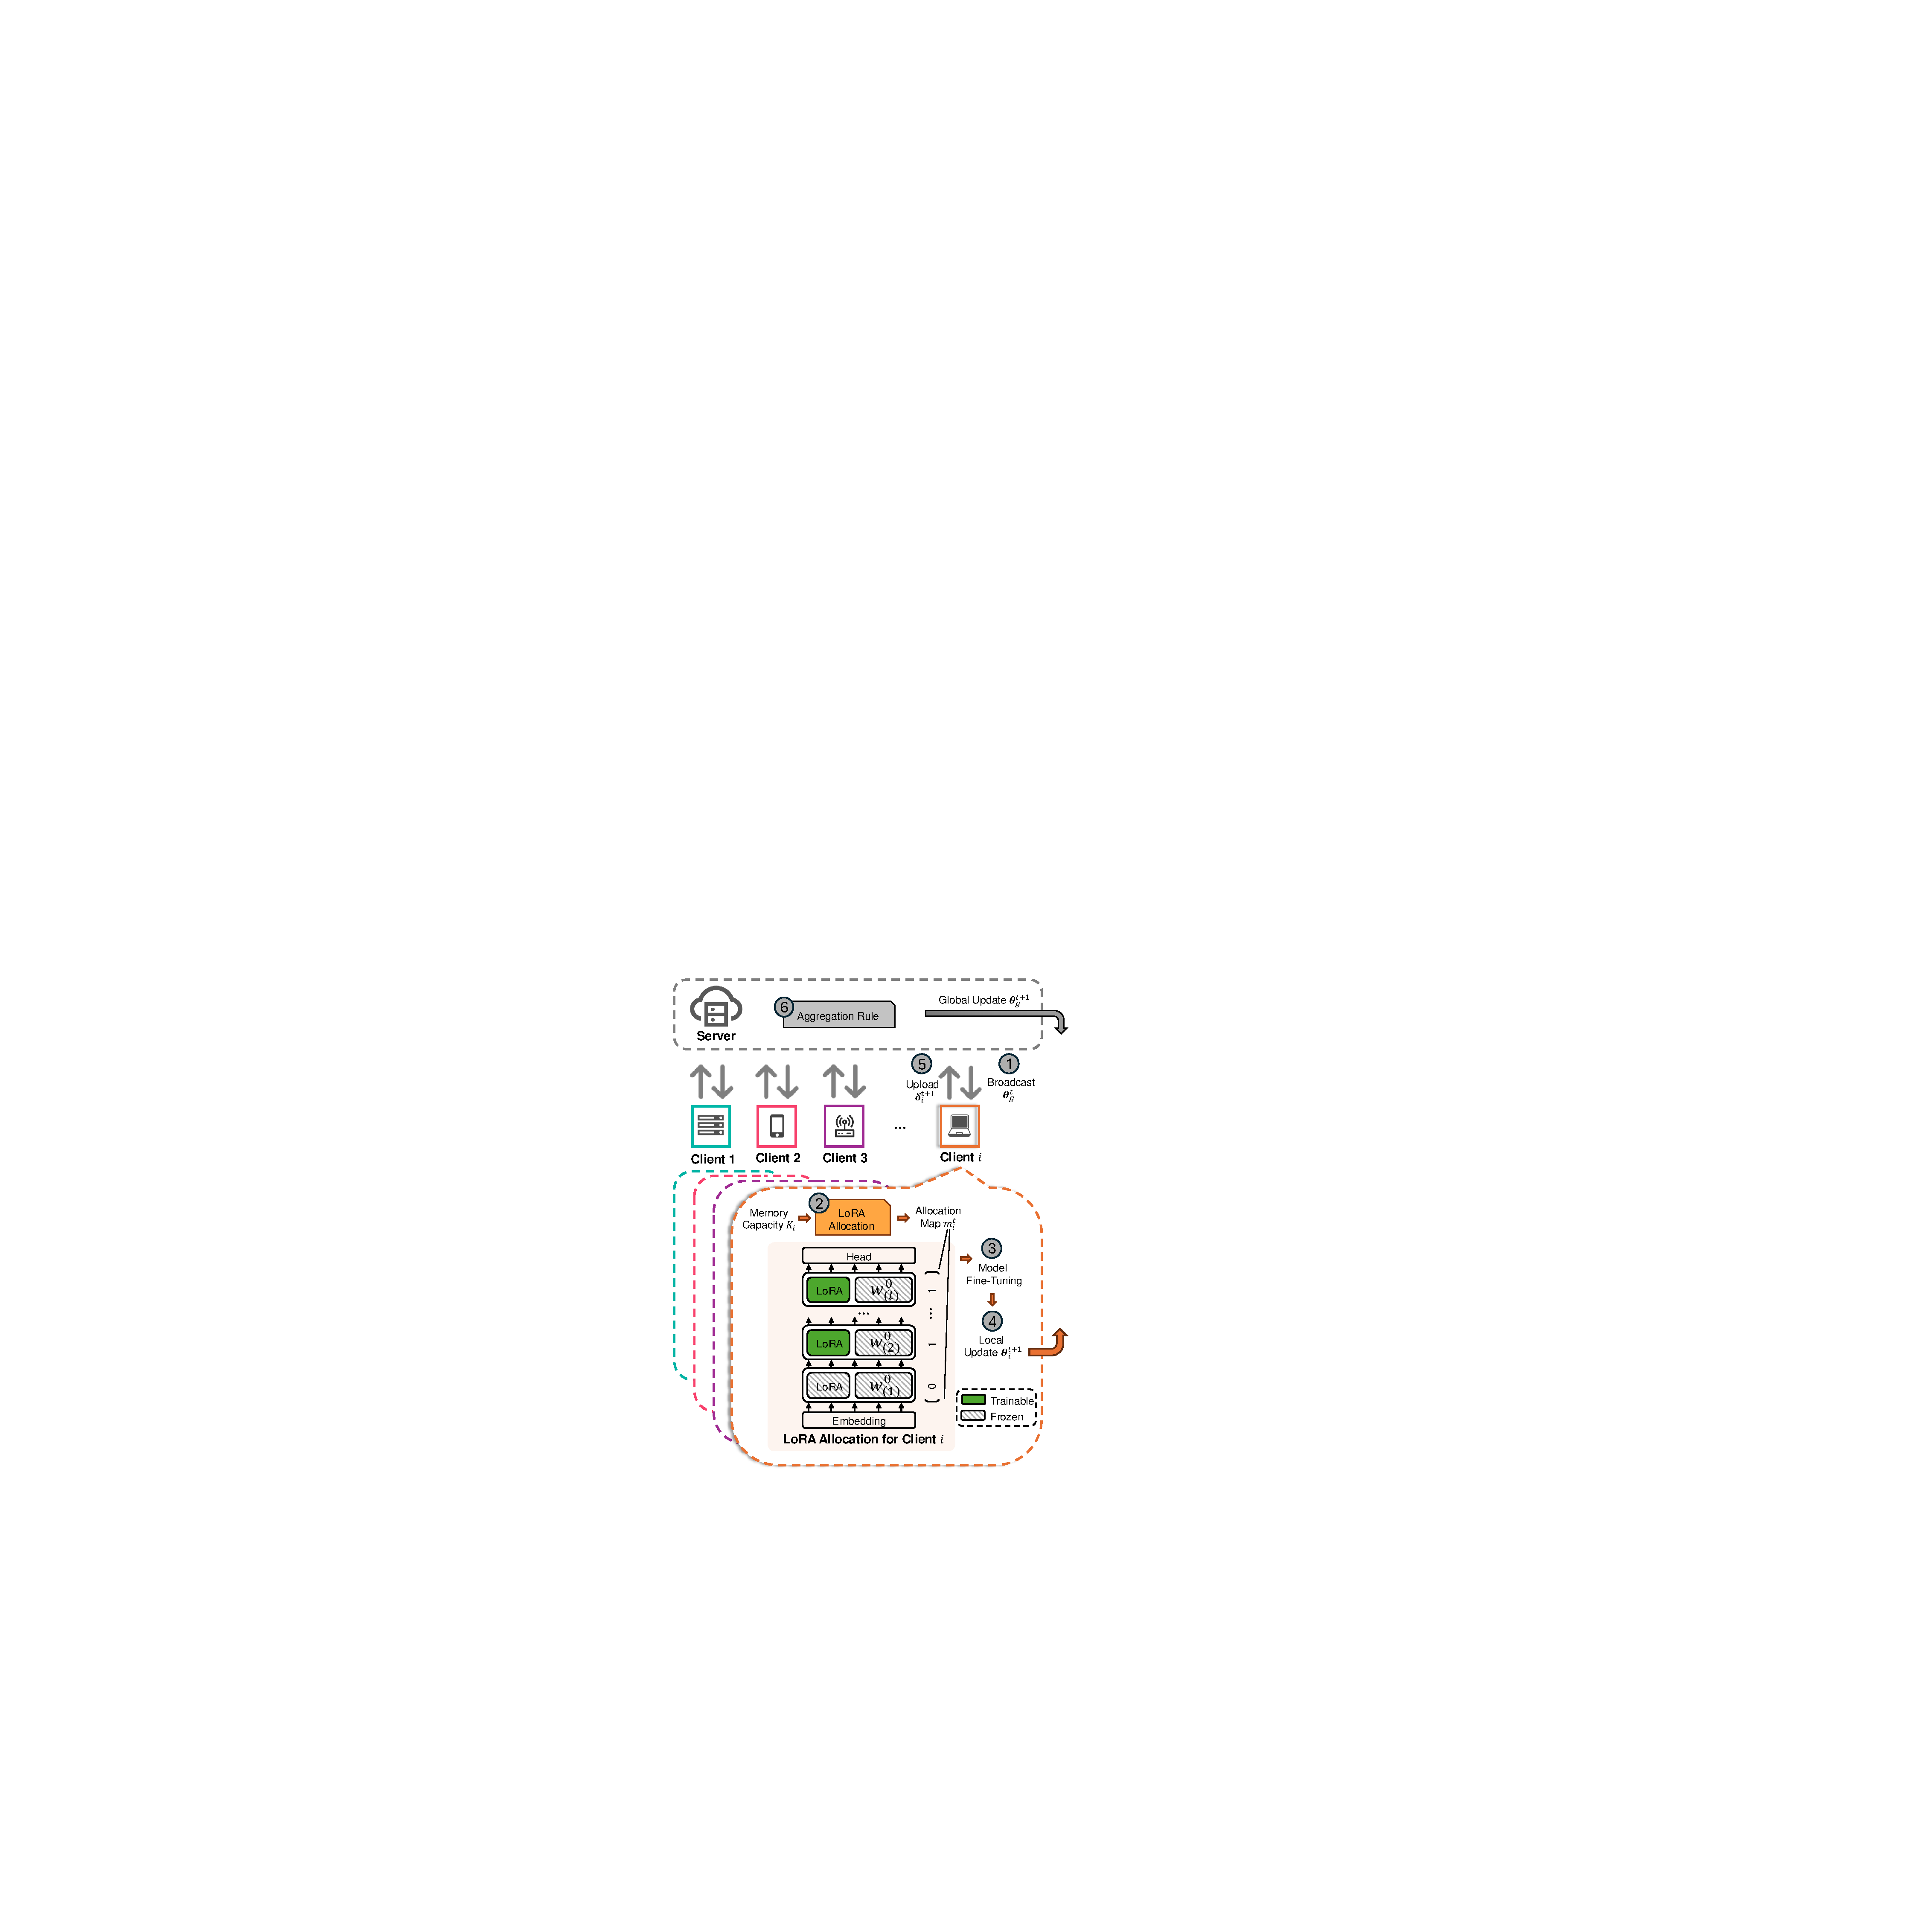
\includegraphics[width=0.38\textwidth]{fig/overallFramework.pdf}
% % \vspace{-10pt}
% \caption{The overall system of Federated Fine-Tuning with heterogeneous clients.}
% \label{appendix-fig:framework}
% \end{figure}

% % In Figure~\ref{appendix-fig:framework}, 
% In Algorithm~\ref{algorithm-ours},
% we illustrate the overall system of Fed-pilot. We describe its process in steps as follows:
% At each round $t\in[T]$, the server broadcasts the current global trainable parameters $\boldsymbol{\mathcal{\theta}}_g^t$ to a subset of $q$ clients, denoted as $\mathbb{Q}^t$. Each client $i$ initializes its local model as $\boldsymbol{\Theta}_i^t=\{\boldsymbol{\mathcal{\theta}}_i^t; \boldsymbol{\Theta}^0 \}$ using the global parameters $\boldsymbol{\mathcal{\theta}}_g^t$
% % , such that $\boldsymbol{\Theta}_i^t=\{\boldsymbol{\mathcal{\theta}}_g^t; \boldsymbol{\Theta}^0 \}$. 
% Given its memory capacity $\mathcal{K}_i$, the client determines the LoRA allocation map $m_i^t$ through an optimization algorithm to maximize global model performance.
% Then, the client fine-tunes $\boldsymbol{\Theta}_i^t$ using its local dataset $D_i$ for layers where $m_{i,{(j)}}^t=1$. The updated parameters $\boldsymbol{\mathcal{\theta}}_i^{t+1}$ are obtained. Each client then uploads its local update $ \boldsymbol{\delta}_i^{t+1} := \boldsymbol{\mathcal{\theta}}_i^{t+1} - \boldsymbol{\mathcal{\theta}}_i^t$, where $m_{i,{(j)}}^t=1$ to the server. The server finally aggregates the updates and computes the global parameter update layer-wise with ComAgg.
% %
% % $\boldsymbol{\mathcal{\theta}}_g^{t+1} := \boldsymbol{\mathcal{\theta}}_g^t + ({1}/{q})\sum_{i\in \mathbb{Q}^t}\boldsymbol{\delta}_i^{t+1},$ which results in the global model $\boldsymbol{\Theta}_g^{t+1}=\{\boldsymbol{\mathcal{\theta}}_g^{t+1};\boldsymbol{\Theta}^0\}$ 
% %
% % \begin{equation}\label{appendix-eq:newagg}
% % \begin{aligned}
% % \boldsymbol{\mathcal{\theta}}_{g, (j)}^{t+1} := \boldsymbol{\mathcal{\theta}}_{g, (j)}^t + \frac{1}{|\mathbb{Q}_{(j)}^t|} \sum_{i \in \mathbb{Q}_{(j)}^t} \boldsymbol{\delta}_{i, (j)}^{t+1},
% % \end{aligned}
% % \end{equation}
% % for the next training round. 
% % where $\mathbb{Q}_{(j)}^t \subseteq \mathbb{Q}^t$ represents the subset of clients that trained the $j$-th LoRA layer at round $t$.
% % This process continues until the global model converges. 
% % We introduce our algorithm in Algorithm~\autoref{algorithm-ours} as well.

% \begin{algorithm}[t]
% \caption{Fed-pilot}\label{algorithm-ours}
% \begin{algorithmic}[1]
% \REQUIRE Pre-trained model $\boldsymbol{\Theta}^0$, trainable LoRA modules $\boldsymbol{\mathcal{\theta}}$, number of clients $v$, memory capability $\mathcal{K}_i, i\in[v]$, number of transformer layers $l$ %IG Score $I_{(j)}$ for $j$-th block.
% % \STATE $\boldsymbol{\Phi} \leftarrow \boldsymbol{\Phi}^0 \hfill \lhd$ Initial global model
% \STATE Initial trainable global model $\boldsymbol{\mathcal{\theta}}^0$
% % \STATE Initial global model $\boldsymbol{\Theta}_g^0=\{\boldsymbol{\mathcal{\theta}}_g^0, \boldsymbol{\Theta}^0 \}$
% % \FOR{each clients $i \in [v]$ \textbf{in parallel}}
% %     \STATE Server broadcasts the initial global model $\boldsymbol{\Theta}_g^0$
% %     \STATE Client saves this model as their initial local models $\boldsymbol{\Theta}_i^0$
% % \ENDFOR
% \FOR{$t=0$ to $T-1$}
%     \STATE Server randomly samples a subset of clients $\mathcal{S}^t$ and broadcasts $\boldsymbol{\mathcal{\theta}}^t$ to them
%     \FOR{each clients $i \in \mathcal{S}^t$ \textbf{in parallel}}
%         \STATE Obtain IG score $G(\boldsymbol{\mathcal{\theta}_{i}})$ as Equation~\ref{eq:valuefunction}
%         \STATE Calculate the optimal allocation map $m_{i}^t=\text{Knapsack}(\mathcal{K}_i, G(\boldsymbol{\mathcal{\theta}_{i}}))$
%         \STATE $\boldsymbol{\delta}_i^{t}$ $\leftarrow \text{LocalUpdate}(\boldsymbol{\mathcal{\theta}}_i^{t},m^t_i)$
%     \ENDFOR
%     % \STATE $\boldsymbol{\mathcal{\theta}}_i^{t+1} \leftarrow \boldsymbol{\mathcal{\theta}}_i^{t}-(1/s)\sum_{i\in[n]}\boldsymbol{\delta}_i^{t}$
%     \STATE $\boldsymbol{\theta}^{t+1}_g \leftarrow$ \text{ComAgg}($\boldsymbol{\delta}^{t+1}$, $\boldsymbol{\delta}^{t}$) by Equation~\ref{eq:agg_temporal}
% \ENDFOR
% \STATE return $\boldsymbol{\Theta}_g^T=\{\boldsymbol{\mathcal{\theta}}_g^T, \boldsymbol{\Theta}^0 \}$
% \end{algorithmic}
% \end{algorithm}

\section{Details on Experimental Settings}\label{sec:appendix-settings}

    \subsection{FL Settings}\label{subsec:appendix-settings-flsettings}

    % Table generated by Excel2LaTeX from sheet 'Sheet2'
    \begin{table}[t]
      \centering
      \caption{FL settings for all experiments.}
      \scalebox{0.65}{
        \begin{tabular}{c|ccccccccc}
        \toprule[1pt]
        \textbf{Dataset/Configuration} & \textbf{Model} & \textbf{LoRA} & \textbf{Client} & \textbf{Training Round} & \textbf{Learning Rate} & \textbf{batch size} & $T_{\text{IG}}$ & $T_{\text{Agg}}$ & $|D_{\text{IG}}|$ \\
        \midrule
        \textbf{Natural Instruction} & Llama (Data-Juicer-1B) & rank=8, lora\_alpha=16, target\_modules=[``q\_proj'', ``v\_proj''] & 50 (10\%) & 6     & 0.00005 & 8     & 1     & 2     & 50 \\
        \textbf{Dolly-15K} & OPT-1.3B & rank=8, lora\_alpha=16, target\_modules=[``q\_proj'', ``v\_proj''] & 50 (10\%) & 25    & 0.00005 & 8     & 2     & 2     & 50 \\
        \textbf{CIFAR-100} & ViT-base & rank=16, lora\_alpha=16, target\_modules=[``query'', ``value''] & 100 (10\%) & 350   & 0.1   & 496   & 10    & 10    & 50 \\
        \textbf{LEDGAR} & BERT-base & rank=16, lora\_alpha=16, target\_modules=[``query'', ``value''] & 100 (10\%) & 350   & 0.01  & 496   & 10    & 10    & 50 \\
        \textbf{DomainNet-121} & ViT-base & rank=16, lora\_alpha=16, target\_modules=[``query'', ``value''] & 100 (10\%) & 350   & 0.05  & 496   & 10    & 10    & 50 \\
        \bottomrule[1pt]
        \end{tabular}%
        }
      \label{tab:appendix-fl-settings}%
    \end{table}%

    % The table~\ref{tab:appendix-fl-settings} presents the datasets, models, LoRA configurations, number of clients, training rounds, learning rates, batch sizes, and key hyperparameters ($N_{\text{IG}}$, $N_H$, and $|D_{\text{IG}}|$). LoRA layers are applied to the specified transformer modules, with rank, and scaling parameters. In FL experiments, we use $v=100$ clients with a local epoch of 1 and training rounds $T=350$. Each round, the server selects $q=10$ clients for local fine-tuning using the AdamW optimizer and a batch size of 8. For all experiments, both $N_{\text{IG}}$ and $N_{\text{H}}$ are set to 10, and $|D_{\text{IG}}|$ is 50.

    % LoRA layers are applied to the ``query'' and ``value'' modules in each transformer layer, with the rank, scaling parameter, and dropout probability set as 16, 16, and 0.1, respectively. 

    % In the FL experiments, we use $v=100$ clients, with the local epoch of 1 and training rounds $T=350$. In each round, the server randomly selects $q=10$ clients for local fine-tuning using the AdamW optimizer and a batch size of 8. 

    % In all experiments, both $N_{\text{IG}}$ and $N_{\text{H}}$ are set to 10, and $|D_{\text{IG}}|$ is 50.

    The table presents the FL settings used for all experiments, detailing the datasets, models, LoRA configurations, client distribution, training rounds, learning rates, batch sizes, and key hyperparameters. It includes five datasets: Natural Instruction, Dolly-15K, CIFAR-100, LEDGAR, and DomainNet-121. Different models were used, including Llama (Data-Juicer-1B), OPT-1.3B, ViT-base, and BERT-base. The LoRA configuration varies by dataset, specifying rank, scaling parameter (lora\_alpha), and target modules such as $q_{\text{proj}}$, $v_{\text{proj}}$, $query$, and $value$. The number of participating clients differs, with CIFAR-100, LEDGAR, and DomainNet-121 using 100 clients (10\% per round), while Natural Instruction and Dolly-15K involve 50 clients (10\% per round). Training rounds range from 6 to 350, with learning rates varying between 0.00005 and 0.1. Batch sizes are set to 8 and 496 for different models. 
    Across all experiments, the local IG dataset size $|D_{\text{IG}}|$ is fixed at 50, while other hyper-parameters are case-by-case.

    \subsection{GPU Memory Capacity Settings}\label{subsec:appendix-capacity-settings}

    % Table generated by Excel2LaTeX from sheet 'Sheet1'
    \begin{table}[t]
      \centering
      \caption{Memory capacity settings and context memory consumptions for heterogeneous client groups.}
      \scalebox{0.85}{
        \begin{tabular}{c|cc|cc|cc|cc}
        \toprule[1pt]
        \multirow{2}[4]{*}{\textbf{Model/Capacity Level}} & \multicolumn{2}{c|}{\textbf{Level 1 (4/10 clients)}} & \multicolumn{2}{c|}{\textbf{Level 2 (3/10)}} & \multicolumn{2}{c|}{\textbf{Level 3 (2/10)}} & \multicolumn{2}{c}{\textbf{Level 4 (1/10)}} \\
    \cmidrule{2-9}          & \textbf{GPU Type} & \textbf{Context (MB)} & \textbf{GPU Type} & \textbf{Context (MB)} & \textbf{GPU Type} & \textbf{Context (MB)} & \textbf{GPU Type} & \multicolumn{1}{c}{\textbf{Context (MB)}} \\
        \midrule
        \textbf{Llama (Data-Juicer-1B)} & V100 32 GB & 80    & A100 40 GB & 1,470  & A6000 48 GB & 2,870  & H100 80 GB & 5,650 \\
        \textbf{OPT-1.3B} & V100 32 GB & 2,890  & A100 40 GB & 4,913  & A6000 48 GB & 6,862  & H100 80 GB & 8,811 \\
        \textbf{ViT-base} & A5000 24 GB & 380   & V100 32 GB & 2,280  & A100 40 GB & 4,170  & A6000 48 GB & 5,800 \\
        \textbf{BERT-base} & A5000 24 GB & 280   & V100 32 GB & 1,962  & A100 40 GB & 3,981  & A6000 48 GB & 5,700 \\
        \bottomrule[1pt]
        \end{tabular}%
        }
      \label{tab:appendix-memory-capacity}%
    \end{table}%

    Table~\ref{tab:appendix-memory-capacity} categorizes memory capacity settings and GPU Context memory consumption for different models across four client levels based on experimental results. Llama (Data-Juicer-1.3B) has the lowest context memory at 80 MB on Level 1 (V100 32 GB) and the highest at 5650 MB on Level 4 (H100 80 GB). OPT-1.3B follows a similar trend, ranging from 2890 MB on Level 1 to 8811 MB on Level 4. ViT-base starts at 380 MB on Level 1 (A5000 24 GB) and increases to 5800 MB on Level 4 (A6000 48 GB). BERT-base consumes the least memory, from 280 MB on Level 1 to 5700 MB on Level 4. These results illustrate the scaling of context memory with GPU capacity and the computational demands of different models under heterogeneous client conditions.

    \uline{The GPU configurations are flexible, and our Knapsack optimization algorithm can be applied to various GPU devices with various memory capacities.}

    \subsection{Experimental Settings for Figure~\ref{fig:motivation}}\label{subsec:appendix-motivation-settings}

    In Figure~\ref{fig:motivation}, we present preliminary experiments to explore how different LoRA allocation strategies impact memory consumption and global model accuracy. The experiments use ViT-base, a transformer-based model with 12 encoder layers, where LoRA is applied to all 12 layers, specifically to the “query” and “value” components. The hyperparameters are set as follows: rank = 16, alpha = 16, and dropout ratio = 0.1. In the FL settings, the total number of users is 100, the selection rate is 10\%, the total training rounds are 350, and the local round is set to 1. The batch size is 496, distributed across 8 GPUs (62 on each GPU). The local learning rate is 0.01, optimized using Adam. Results are evaluated on CIFAR-100 and divided according to an IID distribution.

    % To investigate memory consumption and enable FL for heterogeneous clients, we first break down memory consumption into four components, as shown in Figure.~\ref{fig:motivation} (b). When training a ViT-base~\cite{dosovitskiy2020image} model with 12 transformer layers and applying LoRA to each layer, activation memory accounts for the largest share of the total memory consumption. This memory is required to store activations for back-propagation and predominantly resides in the transformer layers.

    we conduct experiments by training the first 1, first 6, last 1, last 6, and all 12 LoRA modules on the CIFAR-100 dataset, as shown in Figure.~\ref{fig:motivation} (a). These strategies lead to varying memory consumption, which corresponds to different memory capacities commonly seen in real-world NVIDIA GPUs, such as NVIDIA RTX A2000 (12GB), NVIDIA RTX A5000 (24GB), NVIDIA Tesla A100 (40GB), NVIDIA RTX A6000 (48GB). The GPU memory usage is calculated based on the method described in Section~\ref{subsec:appendix-memory-footprint-example}. The memory consumption for contexts with 1, 6, and 12 layers is derived from multiple experimental results and fixed at 100, 2,280, and 5,800 MB, respectively.

    Due to the presence of static activations~\cite{ardakani2024slimfit}, which cannot be discarded because of non-linear functions (e.g., GELU, LayerNorm, and Softmax), the memory consumption for training the first 1 or 6 layers approaches that of training all 12 layers. Additionally, the results reveal a notable performance disparity based on which LoRA modules are trained (e.g., a comparison between the ``Last 6'' and ``First 6'' strategies), highlighting the varying importance of different layers in the model.
    
\section{Details of Dataset}\label{sec:appendix-dataset}

\circled{1} \textbf{Natural Instruction:}
The Natural Instruction dataset~\cite{wang2022super} is a large-scale collection of human-written instructions designed to facilitate instruction-based learning for natural language processing models. It consists of a diverse set of tasks, covering various domains such as classification, summarization, translation, question answering, and reasoning. The dataset consists of 1,616 diverse natural language tasks with instructions and answers. 
In our experiments, data instances are formatted into prompts before being processed by the LLMs. We utilize the template provided by Alpaca~\cite{taori2023stanford} to format the datasets used in our experiments.
In the pre-processing, we first filter out tokens with a total length larger than 512, which results in 613 tasks, with 50,348 training samples, and 5,517 testing samples. 
%
% We use Natural Instruction (NI) dataset~\cite{wang2022super} and Dolly-15K~\cite{conover2023free} dataset to evaluate how task heterogeneity affect the performance, respectively.
% % The NI dataset consists of 1,616 diverse natural language tasks with instructions,  and answers. 
We simulate three levels of task heterogeneity from IID to extreme Non-IID, by varying the number of client's data tasks to full, 20, and 15 for NI.
% and full, 3, and 1 for Dolly-15K. 
% The Dolly-15K dataset is a instructiona-following record dataset that generated by human and Wikipedia. 
% The Dolly-15K dataset includes 8 tasks with instructions, contexts, and responses.
% Considering the limited device resources, we take Llama-like model DataJuicer~\cite{chen2024data} and OPT-1.3B~\cite{zhang2022opt} as the foundation models. All reported results are based on the metric called Rough-L.
% \textbf{Category Heterogeneity.} To evaluate the impact of category heterogeneity by skewing the labels, we conduct experiments on CIFAR-100 dataset~\cite{krizhevsky2009learning} and LEDGAR dataset from LexGLUE~\cite{chalkidis-etal-2021-lexglue}. 
% Each of the dataset has 100 categories with visual or text objects, respectively. 
% We skew the datasets by assigning 20, and 10 categories of data samples for each client to fully evaluate the real-world category heterogeneity effects. We take ViT-base~\cite{dosovitskiy2020image} for visual tasks and BERT-base~\cite{devlin2019bert} for language tasks. Results are reported in Accuracy for visual tasks and in Macro F1 for language tasks.
% \textbf{Domain Heterogeneity.} Domain discrepancy is commonly seen in the dataset from distributed clients, we implement experiments on a customized DomainNet dataset~\cite{peng2019moment} (referred to as DomainNet-121). In the dataset, there are six visual domains including clipart, real-world images, sketch, infograph, painting, and quickdraw. For each client, we only assign one domain and with number of categories varying from full, 50, and 25. All results are reported with Accuracy.

\circled{2} \textbf{Dolly-15K:} The Dolly-15K dataset~\cite{conover2023free} is an open-source instruction-tuning dataset introduced by Databricks to improve the fine-tuning of large language models for instruction-following tasks. It comprises 15,000 human-generated prompt-response pairs spanning diverse domains such as open-ended question answering, summarization, brainstorming, and information extraction. Unlike many instruction-tuning datasets that rely on synthetic data, Dolly-15K ensures high-quality, natural language interactions through human-authored responses, making it a valuable resource for training and evaluating instruction-following models.
For preprocessing, we applied the same prompts as in the NI dataset and filtered out samples exceeding 512 tokens in total length. This resulted in 10,936 training and 2,735 testing samples. To simulate different levels of task heterogeneity, we varied the number of tasks per client, creating three settings: IID (full task set per client), mild Non-IID (3 tasks per client), and extreme Non-IID (1 task per client).
% Dolly-15K~\cite{conover2023free} is a publicly available instruction-tuning dataset introduced by Databricks to enhance the fine-tuning of large language models for instruction-following tasks. It consists of 15,000 human-generated prompt-response pairs covering a wide range of domains, including open-ended question answering, summarization, brainstorming, and information extraction. Unlike many instruction-tuning datasets that rely on model-generated synthetic data, Dolly-15K was created to ensure high-quality, diverse, and natural language interactions. The dataset serves as a valuable resource for training and evaluating models in instruction-following capabilities, particularly in scenarios where human-like responses are required.
% We applied the same Prompt as in NI dataset, and pre-process the dataset by filtering out the sample that total length excceds the 512. It results in 10,936 training data and 2735 testing data.
% We simulate three levels of task heterogeneity from IID to extreme Non-IID, by varying the number of client's data tasks to full, 3, and 1 for Dolly-15K. 

\circled{3} \textbf{CIFAR-100:} The CIFAR-100 dataset consists of 60,000 32$\times$32 color images in 100 classes, with 600 images per class. There are 500 training images and 100 testing images per class. For the Non-IID data distribution, we apply quantity and label skews to the dataset. For quantity skew, we use Dirichlet with $\alpha=1.0$, and for label skew, we use pathological where the data on each client only contains the specific number of labels. This results in three levels of data distribution: $\{IID, (20/Dir\sim1.0), (10/Dir\sim1.0)\}$, where $(20/Dir\sim1.0)$ means each client only contains 20 out of 100 categories of samples, and the number of samples obeys the Dirichlet distribution with $\alpha=1.0$. 

\circled{4} \textbf{LEDGAR-100:} The LEDGAR dataset aims at contract provision classification. The contract provisions sourced from contracts obtained from the US Securities and Exchange Commission filings, which are publicly available from EDGAR. Each category represents the single main topic of the corresponding contract provision. There are 100 categories, with 60,000 samples for training and 10,000 for testing. The number of samples for each category is unbalanced. The data distribution skew is the same as that of CIFAR-100. 

\circled{5} \textbf{DomainNet-121:} The original DomainNet is a dataset of common objects in six different domains. All domains include 345 categories of objects and a total of {424.5k} images. The domains include clipart, real, sketch, infograph, painting, and quickdraw. We craft DomainNet-121 by selecting categories that all six domains have more than 50 images, resulting in 121 categories. Then, we randomly choose 50 images per category per domain, resulting in 300 images per category. Subsequently, we sample 5 images from each category in each domain for testing. There are 270 training images and 30 testing images per class. For Non-IID data distribution, we apply domain and category skews: $\{1D/121C, 1D/50C, 1D/25C)\}$, where $1D/121$ means each client contains 121 out of 121 categories and 1 out of 6 domains of samples.  

More specifically, the categories drawn from the original DomainNet are as follows:

\begin{multicols}{4}
\noindent
barn\\
baseball\_bat\\
basket\\
beach\\
bear\\
beard\\
bee\\
bird\\
blueberry\\
bowtie\\
bracelet\\
brain\\
bread\\
broccoli\\
bus\\
butterfly\\
circle\\
cloud\\
cruise\_ship\\
dolphin\\
dumbbell\\
elephant\\
eye\\
eyeglasses\\
feather\\
fish\\
flower\\
foot\\
frog\\
giraffe\\
goatee\\
golf\_club\\
grapes\\
grass\\
guitar\\
hamburger\\
hand\\
hat\\
headphones\\
helicopter\\
hexagon\\
hockey\_stick\\
horse\\
hourglass\\
house\\
ice\_cream\\
jacket\\
ladder\\
leg\\
lipstick\\
megaphone\\
monkey\\
moon\\
mushroom\\
necklace\\
owl\\
panda\\
pear\\
peas\\
penguin\\
pig\\
pillow\\
pineapple\\
pizza\\
pool\\
popsicle\\
rabbit\\
rhinoceros\\
rifle\\
river\\
sailboat\\
sandwich\\
sea\_turtle\\
shark\\
shoe\\
skyscraper\\
snorkel\\
snowman\\
soccer\_ball\\
speedboat\\
spider\\
spoon\\
square\\
squirrel\\
stethoscope\\
strawberry\\
streetlight\\
submarine\\
suitcase\\
sun\\
sweater\\
sword\\
table\\
teapot\\
teddy-bear\\
telephone\\
tent\\
The\_Eiffel\_Tower\\
The\_Great\_Wall\_of\_China\\
The\_Mona\_Lisa\\
tiger\\
toaster\\
tooth\\
tornado\\
tractor\\
train\\
tree\\
triangle\\
trombone\\
truck\\
trumpet\\
umbrella\\
vase\\
violin\\
watermelon\\
whale\\
windmill\\
wine\_glass\\
yoga\\
zebra\\
zigzag
\end{multicols}

\textbf{Metric for each dataset.} For NI and Dolly-15K datasets, we use the Rouge-L metric. Rouge-L (Recall-Oriented Understudy for Gisting Evaluation - Longest Common Subsequence) is a widely used metric for evaluating the quality of text generated by large language models, particularly in summarization and text generation tasks. Unlike Rouge-N, which measures exact n-gram overlap, Rouge-L focuses on the Longest Common Subsequence (LCS) between the generated text and the reference text, capturing sentence-level fluency and coherence. Since LCS does not require consecutive word matches, it is better suited for evaluating paraphrased or loosely structured responses. The Rouge-L score consists of precision, recall, and F1-score, providing a balanced measure of how well the generated text aligns with the reference while allowing for flexible word order. This makes it particularly useful for assessing LLM outputs in real-world applications where exact phrasing may vary while preserving meaning. For CIFAR-100 and DomainNet-121 datasets, we evaluate the performance using accuracy, defined as the ratio of the number of correct predictions to the total number of predictions, i.e., $\text{Accuracy} = \frac{\text{Number of Correct Predictions}}{\text{Total Number of Predictions}} \times 100\%$.
In the case of the LEDGAR dataset, we compute the metrics Micro F1 and Macro F1. Micro F1 is calculated as: $\frac{2 \times \text{Micro Precision} \times \text{Micro Recall}}{\text{Micro Precision} + \text{Micro Recall}}$, where Micro Precision and Micro Recall are defined as $\frac{\sum_{i=1}^{N} TP_i}{\sum_{i=1}^{N} (TP_i + FP_i)}$ and $\frac{\sum_{i=1}^{N} TP_i}{\sum_{i=1}^{N} (TP_i + FN_i)}$, respectively. Here, $TP_i$ is the number of true positive predictions for class $i$, $FP_i$ is the number of false positive predictions for class $i$, $N$ is the total number of classes. On the other hand, Macro F1 is calculated individually for each class. It is computed by replacing Micro Precision and Micro Recall with Macro Precision and Macro Recall which are defined as, $\frac{1}{N} \sum_{i=1}^{N} \frac{TP_i}{TP_i + FP_i}$ and $\frac{1}{N} \sum_{i=1}^{N} \frac{TP_i}{TP_i + FN_i}$, respectively. We use the Macro F1 score to evaluate the best result for the LEDGAR dataset.

\section{More Results}\label{sec:appendix-results-visualization}



\begin{figure}[t]
\centering
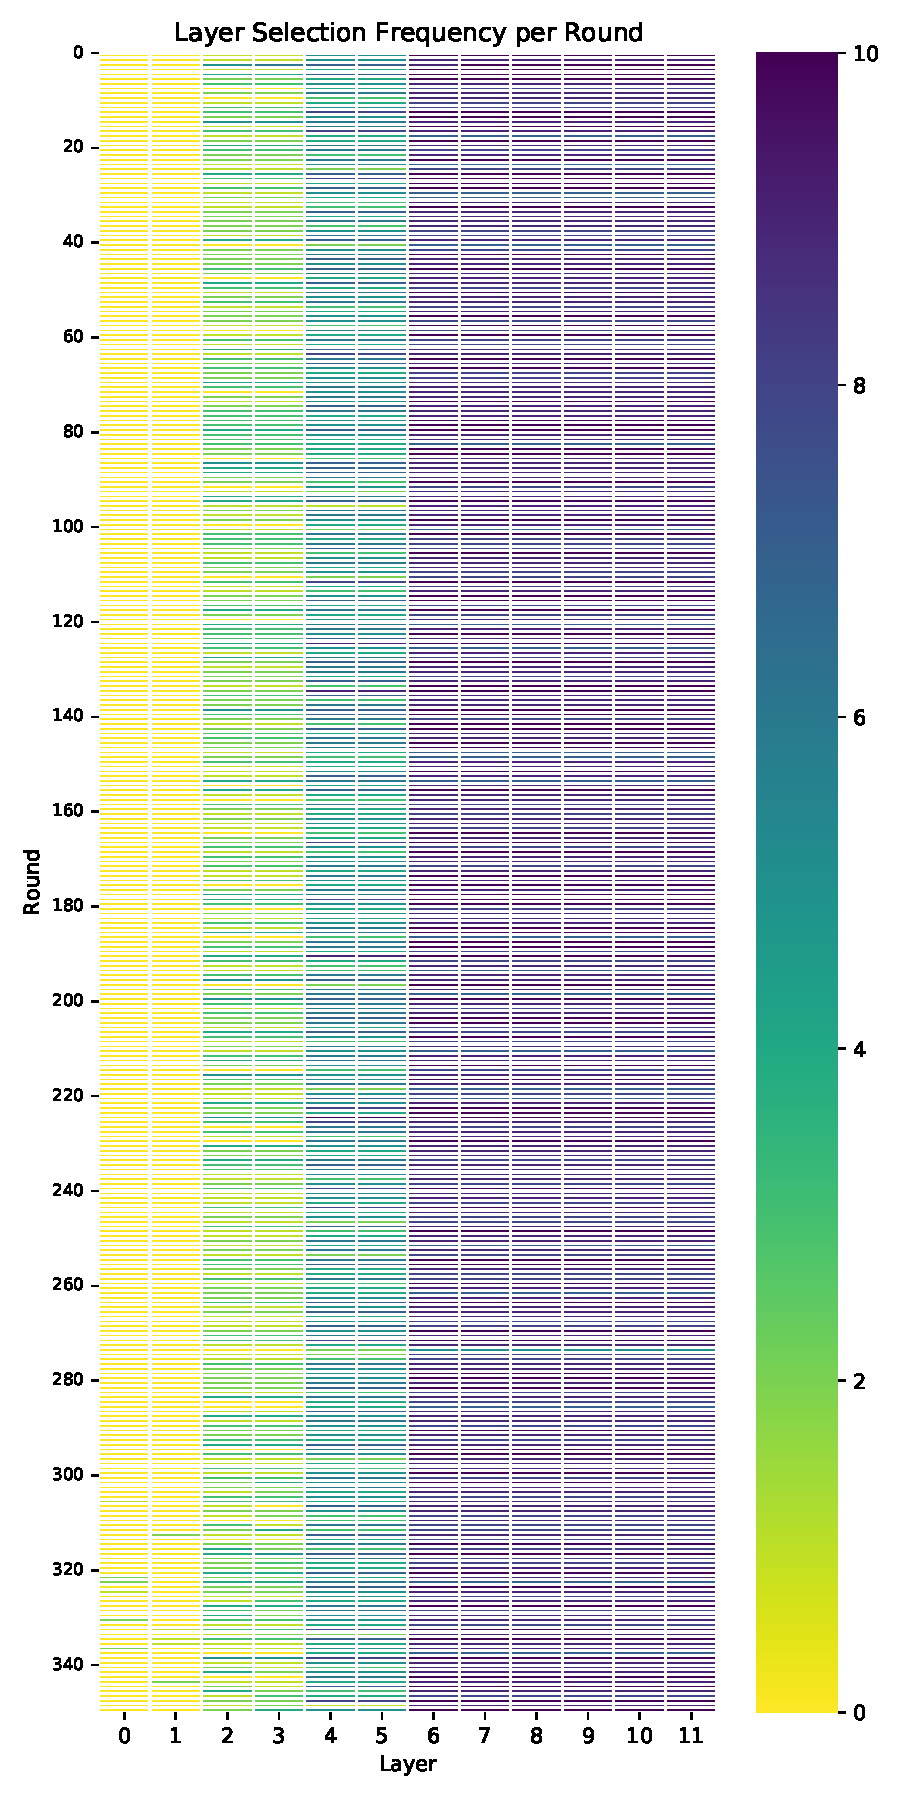
\includegraphics[width=0.45\textwidth]{fig/layer-selection.pdf}
% \vspace{-10pt}
\caption{The selection frequency of LoRA modules in each attention layer across rounds.}
\label{fig:layerselection}
\end{figure}

\textbf{The LoRA Module Allocation Frequency.} We visualize the selection frequency of LoRA modules in each attention layer across training rounds. The experiment is conducted on the CIFAR-100 dataset under the Non-IID (10) setting. As shown in Figure~\ref{fig:layerselection}, our allocation optimization algorithm demonstrates stable LoRA selection patterns across rounds. The last six layers (layers 6 to 11) are most frequently selected throughout training. Layers 4 and 5 are chosen more often than layers 2 and 3 in most rounds. The first two layers are selected less frequently due to their higher memory consumption but are occasionally chosen in later rounds as other layers converge.

\section{Comparative Study on Related Works}\label{sec:appendix-comparative_study}

\begin{table}[t]
  \centering
  \caption{A comparative study with state-of-the-art works.}
  \scalebox{0.90}{
    \begin{tabular}{ccccccccc}
    \toprule[1pt]
    \textbf{Method}   & \textbf{PEFT} & \textbf{Resource Heterogeneity} & \textbf{Parameter Heterogeneity} & \textbf{Dynamic Training}  \\\hline
    % {DP-LoRA~\cite{liu2023differentially}}                      & {\ding{51}}        & {\ding{55}}        & {\ding{55}}        & {\ding{55}}                \\
    {FedIT~\cite{zhang2023towards}}               & {\ding{51}}        & {\ding{55}}        & {\ding{55}}         & {\ding{55}}                   \\
    {SLoRA~\cite{babakniya2023slora}}                      & {\ding{51}}        & {\ding{55}}        & {\ding{55}}        &  {\ding{55}}                \\
    {FedMS~\cite{wu2024fedfmsl}}                      &{\ding{51}}         & {\ding{55}}        & {\ding{55}}        &  {\ding{51}}                 \\
    {FwdLLM~\cite{xu2024fwdllm}}                     & {\ding{51}}        & {\ding{55}}        & {\ding{55}}        & {\ding{55}}                  \\
    % {FedBiOT~\cite{wu2024fedbiot}}                     &{\ding{51}}         & {\ding{55}}        &{\ding{55}}         & {\ding{51}}                 \\
    {FFA-LoRA~\cite{sun2024improving}}                      & {\ding{51}}        & {\ding{55}}        & {\ding{55}}        & {\ding{55}}                  \\
    HETLoRA~\cite{cho2024heterogeneous}                   & {\ding{51}}        & {\ding{51}}        & {\ding{51}}        &  {\ding{55}}              \\
    {FLoRA~\cite{wangflora}}                          & {\ding{51}}        & {\ding{51}}        & {\ding{51}}        & {\ding{55}}               \\
    {FlexLoRA~\cite{bai2024federated}}                         & {\ding{51}}        & {\ding{51}}        & {\ding{51}}        & {\ding{55}}               \\
    {FedRA~\cite{su2023fedra}}                          &{\ding{51}}         & {\ding{51}}        & {\ding{51}}        & {\ding{55}}                 \\
    \midrule
    \textbf{{Ours}}                   & {\ding{51}} & {\ding{51}} & {\ding{51}} & {\ding{51}}  \\
    \bottomrule[1pt]
    \end{tabular}%
    }
  \label{tab:survey}%
\end{table}%

In this section, we compare our approach with existing methods that are related to ours in terms of technical aspects and objectives.
%
% PEFT can be mainly categorized into two types: additive and selective. Additive PEFT methods introduce new trainable layers to the model while keeping the pre-trained model weights frozen, enabling efficient task-specific fine-tuning. For example, prompt tuning~\cite{lester2021power} adds task-specific soft prompts, which are then fine-tuned to adapt the model to new tasks. 
%
% Selective PEFT methods update only a subset of the pre-trained model's parameters. For instance, BitFit~\cite{zaken2022bitfit} updates only the bias parameters, while LN-Norm~\cite{basu2024strong} updates the layer normalization parameters in vision transformer (ViT) models. Further advancements have been made with hybrid approaches that combine multiple PEFT techniques to enhance fine-tuning efficiency~\cite{he2021towards, zhou2023autopeft}. Among these PEFT methods, LoRA has demonstrated more stable and effective performance~\cite{ding2022delta, zhang2023fedpetuning}. Without loss of generality, we focus on LoRA in this work. 
%
In Table~\ref{tab:survey}, we present a comparative analysis of our method against state-of-the-art approaches in federated fine-tuning. The comparison considers four key aspects: whether is a PEFT (Parameter-Efficient Fine-Tuning)-based method, whether considers resource heterogeneity, whether considers trainable parameter heterogeneity, and whether incorporate dynamic training. While all listed methods support PEFT, most do not address resource heterogeneity, limiting their adaptability to devices with varying memory capacities. Methods such as HETLoRA, FLoRA, and FlexLoRA incorporate trainable parameter heterogeneity, allowing clients to train LoRA modules with different ranks, but they fail to accommodate resource constraints effectively. Additionally, only a few methods, including FedMS and FedBiOT, support dynamic training, where models can adapt their configurations during training. Our proposed method is the only approach that simultaneously supports PEFT, resource heterogeneity, trainable parameter heterogeneity, and dynamic training, making it a more flexible and scalable solution for federated fine-tuning in heterogeneous environments.

\section{Limitations}\label{sec:appendix-limitation}

Our LoRA allocation optimization is highly adaptable to various memory capacity levels, supporting devices ranging from consumer-grade GPUs to datacenter-grade GPUs. However, if a client cannot train even a single LoRA module, our method can easily combined with other techniques, such as offloading~\cite{kar2023offloading}, checkpointing~\cite{rasley2020deepspeed} to ensure participation without exceeding hardware limitations.

\section{Future Work}\label{sec:appendix-futurework}

{Our method is orthogonal to aggregation noise-reduction techniques} such as FlexLoRA~\cite{bai2024federated} and FLoRA~\cite{wangflora}, allowing for seamless integration to heterogeneous model aggregation. In future work, we plan to incorporate these methods while preserving optimal LoRA allocation across heterogeneous devices.


\end{document}


% This document was modified from the file originally made available by
% Pat Langley and Andrea Danyluk for ICML-2K. This version was created
% by Iain Murray in 2018, and modified by Alexandre Bouchard in
% 2019 and 2021 and by Csaba Szepesvari, Gang Niu and Sivan Sabato in 2022.
% Modified again in 2023 and 2024 by Sivan Sabato and Jonathan Scarlett.
% Previous contributors include Dan Roy, Lise Getoor and Tobias
% Scheffer, which was slightly modified from the 2010 version by
% Thorsten Joachims & Johannes Fuernkranz, slightly modified from the
% 2009 version by Kiri Wagstaff and Sam Roweis's 2008 version, which is
% slightly modified from Prasad Tadepalli's 2007 version which is a
% lightly changed version of the previous year's version by Andrew
% Moore, which was in turn edited from those of Kristian Kersting and
% Codrina Lauth. Alex Smola contributed to the algorithmic style files.
